\documentclass{scrbook} % <= Druckversion: "scrbook" / Bildschirmversion: "scrreprt"
\usepackage[ngerman,bibtex]{osm-thesis} % <= Sprache der Arbeit ("ngerman"/"english"), Biblatex-Backend ("bibtex"/"biber")

% ABOUT
\newcommand{\hpitype}{Bachelorarbeit}
\newcommand{\hpiauthor}{Christian J. Raue}
\newcommand{\hpititle}{Entwicklung und Implementierung von regelmäßigen, randomisierten und bedarfsorientierten Abfahrtsplänen für Züge in einer Verkehrssimulation}
\newcommand{\hpititleother}{Development and implementation of regular, randomized and demand-driven departure schedules for trains in a traffic simulation} % <= das Studienreferat verlangt einen deutschen UND englischen Titel
\newcommand{\hpisupervisor}{Prof.\,Dr.\,Andreas Polze, Arne Boockmeyer, Lukas Pirl}
\newcommand{\hpichair}{Professur für Betriebssysteme und Middleware}
\newcommand{\hpiexternalsupervisor}{Henry Huebler, Götz Gassauer}
\newcommand{\hpiexternal}{DB Systel GmbH}
\newcommand{\hpidate}{\today}

% DOCUMENT
\bibliography{bibliography}


\begin{document}

	% Einband
	\pagenumbering{alph}
	\ifisbook\begin{titlepage}
	\setlength{\evensidemargin}{0.5\evensidemargin+0.5\oddsidemargin}
	\setlength{\oddsidemargin}{\evensidemargin}

	\centering

	\raisebox{-0.5\height}{
\includegraphics[width=5.5cm]{images/hpi_logo_black.pdf}}
	\hspace*{.2\textwidth}
	\raisebox{-0.5\height}{
\includegraphics[width=4cm]{images/uni_logo_black.pdf}}
	
	\vspace*{4\baselineskip}
	{\usekomafont{subject}\hpitype}\par
	
	\vfill
	{\usekomafont{title}\hpititle\par}
	\vspace*{\baselineskip}
	{\usekomafont{subtitle}\hpititleother}\par
	
	\vfill
	{\textbf{\phantom{\iflanguage{ngerman}{von}{by}}} \\
	 \smallskip\usekomafont{author}\hpiauthor}\par
	
	\vfill
	\phantom{\begin{minipage}{\textwidth}
	{\textbf{\iflanguage{ngerman}{Betreuung}{Supervisors}}\\
	\usekomafont{publishers}\smallskip\hpisupervisor\\ \textit{\hpichair}\\ \smallskip\textbf{\normalfont\hpiexternalsupervisor}\\ \textit{\hpiexternal}}
	\end{minipage}}
	
	\vfill
	{\usekomafont{date}\iflanguage{ngerman}{Hasso-Plattner-Institut an der Universität Potsdam}{Hasso Plattner Institute at University of Potsdam}}\par
	\vspace*{\baselineskip}
	{\usekomafont{date}\hpidate}\par
	
\end{titlepage}\fi
	\ifisbook\cleardoubleemptypage\fi
	
	% (Haupt-)Titelseite, Abstract, ggf. Danksagung & Inhaltsverzeichnis
	\pagenumbering{roman}
	\begin{titlepage}
	\centering

	\raisebox{-0.5\height}{
\includegraphics[width=5.5cm]{images/hpi_logo_srgb.pdf}}
	\hspace*{.2\textwidth}
	\raisebox{-0.5\height}{
\includegraphics[width=4cm]{images/uni_logo_srgb.pdf}}

	\vspace*{4\baselineskip}
	{\usekomafont{subject}\hpitype}\par
	
	\vfill
	{\usekomafont{title}\hpititle\par}
	\vspace*{\baselineskip}
	{\usekomafont{subtitle}\hpititleother}\par
	
	\vfill
	{\textbf{\iflanguage{ngerman}{von}{by}}\\ 
		\smallskip\usekomafont{author}\hpiauthor}\par
	
	\vfill
	{\textbf{\iflanguage{ngerman}{Betreuung}{Supervisors}}\\ 
		\usekomafont{publishers}\smallskip\hpisupervisor\\ \textit{\hpichair}\\ \smallskip\textbf{\normalfont\hpiexternalsupervisor}\\ \textit{\hpiexternal}}
	
	\vfill
	{\usekomafont{date}\iflanguage{ngerman}{Hasso-Plattner-Institut an der Universität Potsdam}{Hasso Plattner Institute at University of Potsdam}}\par
	\vspace*{\baselineskip}
	{\usekomafont{date}\hpidate}\par

	\setcounter{page}{1}

\end{titlepage}


	\ifisbook\cleardoubleemptypage\fi% => Wenn die Arbeit auf Deutsch verfasst wurde, verlangt das Studienreferat KEINEN englischen Abstract

% % englischer Abstract
%\null\vfil
%\begin{otherlanguage}{english}
%\begin{center}\textsf{\textbf{\abstractname}}\end{center}
%
%\noindent Lorem ipsum dolor sit amet, consetetur sadipscing elitr, sed diam nonumy eirmod tempor invidunt ut labore et dolore magna aliquyam erat, sed diam voluptua. At vero eos et accusam et justo duo dolores et ea rebum. Stet clita kasd gubergren, no sea takimata sanctus est Lorem ipsum dolor sit amet. Lorem ipsum dolor sit amet, consetetur sadipscing elitr, sed diam nonumy eirmod tempor invidunt ut labore et dolore magna aliquyam erat, sed diam voluptua. At vero eos et accusam et justo duo dolores et ea rebum. Stet clita kasd gubergren, no sea takimata sanctus est Lorem ipsum dolor sit amet.
%
%\end{otherlanguage}
%\vfil\null


% => Wenn die Arbeit auf Englisch verfasst wurde, verlangt das Studienreferat einen englischen UND deutschen Abstract (der dt. Abstract kann dann ggf. auch ans Ende der Arbeit)

% deutsche Zusammenfassung
\null\vfil
\begin{otherlanguage}{ngerman}
\begin{center}\textsf{\textbf{\abstractname}}\end{center}

\noindent Das Projekt \emph{FlexiDug} erforscht die Nachnutzungsmöglichkeiten der Schieneninfrastruktur, die bisher dem Braunkohletransport in der Lausitz diente. Ziel ist es, ein Konzept für eine gemeinsame Nutzung für Personen- und Güterzüge zu erstellen. Diese Arbeit ist Teil eines Softwareprojekts, das die Simulation des Zugverkehrs auf Basis einer Erweiterung des Verkehrssimulators \emph{SUMO} ermöglicht. Die Arbeit beschäftigt sich mit der Erzeugung von Zügen innerhalb der Simulation. Dafür werden drei verschiedene Arten von Abfahrtsplänen benötigt: regelmäßige, zufällige und bedarfsorientierte. Bedarsforientierte Abfahrtspläne basieren auf dem berechneten Kohlebedarf von Kraftwerken. Die Berechnung basiert auf Stromproduktionsdaten der Bundesntzagentur. Die Ergebnisse der Simulation zeigen, dass die Abfahrtsperioden der Kohlezüge mit dem Kohlebedarf korrelieren und dass die Software einen realistischen Zugverkehr simulieren kann.

\end{otherlanguage}
\vfil\null




	%\ifisbook\cleardoubleemptypage\fi\vspace*{\fill}
\begin{center}\textsf{\textbf{Danksagung}}\end{center}

\noindent Lorem ipsum dolor sit amet, consetetur sadipscing elitr, sed diam nonumy eirmod tempor invidunt ut labore et dolore magna aliquyam erat, sed diam voluptua. At vero eos et accusam et justo duo dolores et ea rebum.

\vspace*{\fill}
	\tableofcontents
	\cleardoublepage

	% Textteil
	\pagenumbering{arabic}

	\chapter{Einleitung}
	\section{Strukturwandel in der Lausitz}
Die Lausitz, eine Region in Südbrandenburg, steht vor in naher Zukunft vor tiefgreifenden Veränderungen. Einer der wichtigsten Wirtschaftsfaktoren in der Region ist der Abbau von Braunkohle durch die LEAG AG in mehreren Tagebauen. Braunkohle ist ein wichtiger Energieträger für die Strom- und Fernwärmeproduktion in der Lausitz. Im Rahmen der Energiewende soll jedoch die Energieproduktion aus Braunkohle bis zum Jahr 2038 zugunsten von erneuerbaren Energiequellen vollständig eingestellt werden. Dies wird die Region  (und auch ganz Deutschland) vor eine Vielzahl von finanziellen, wirtschaftlichen und gesellschaftlichen Herausforderungen stellen. Es müssen neue Wirtschaftskonzepte für die Region entwickelt werden, um diesen Strukturwandel zu bewältigen. Dazu zählt zum einen eine Alternative für den Bergbau zu finden, um den vorhandenen Arbeitnehmern weiterhin Arbeitsplätze zur Verfügung stellen zu können. Die Region möchte weiterhin den Tourismus stark ausbauen durch Nachnutzung der entstehenden Flächen als Erholungsgebiet. Um das erreichen zu können ist es notwendig, die Tagebaulandschaft zu renaturieren und die notwendigen Flächen und Infrastrukturen zu erschließen. Dieser Strukturwandel stellt für die Lausitz den größten Wandel seit dem Strukturbruch im Jahr 1990 im Rahmen der Wiedervereinigung dar. 

Es ist daher notwendig, die entsprechenden Maßnahmen ausreichend zu planen und mit den jeweiligen Interessenvertretern abzustimmen. Mit einem Teil dieser Planung beschäftigt sich das Projekt FlexiDug. Es erkundet Nachnutzungsmöglichkeiten der Schieneninfrastruktur, welche bisher ausschließlich dem Transport der Braunkohle diente und aktuell in privater Hand liegt.
	\section{Das Schienennetz der LEAG}

Essentiell für den Betrieb der Kraftwerke ist die regelmäßige und zuverlässige Belieferung mit Braunkohle. Zu diesem Zweck betreibt die LEAG  ein Schienennetz von 391 Kilometern Länge\cite{hertzer_eisenbahner_2018}. Es verbindet die Tagebaue \emph{Jänschwalde}, \emph{Welzow-Süd}, \emph{Nochten} und \emph{Reichwalde} mit den Braunkohlekraftwerken \emph{Jänschwalde}, \emph{Boxberg} und \emph{Schwarze Pumpe}. Außerdem ist der Kohleveredelungsbetrieb in \emph{Schwarze Pumpe} angeschlossen\cite{noauthor_tagebau_2023}. Gleichzeitig fahren bis zu 25 Kohlezüge auf dem Netz. Sie dienen nicht nur allein dem Transport der Kohle. Ebenso befördern sie die Abfallprodukte der Kohleverstromung, Asche und Gips. Mit ca. 1600 Tonnen pro Zug erreichen sie eine Maximalgeschwindigkeit von 50 km/h und einen Bremsweg von 400 Metern. Zum Fuhrpark gehören 61 E-Loks und 14 Diesel-Loks\cite{hertzer_eisenbahner_2018}. \autoref{fig:leag-netz} zeigt das Schienennetz der LEAG und die Positionen der angeschlossenen Tagebaue und Kraftwerke.

\begin{figure}[!ht]
	\centering
	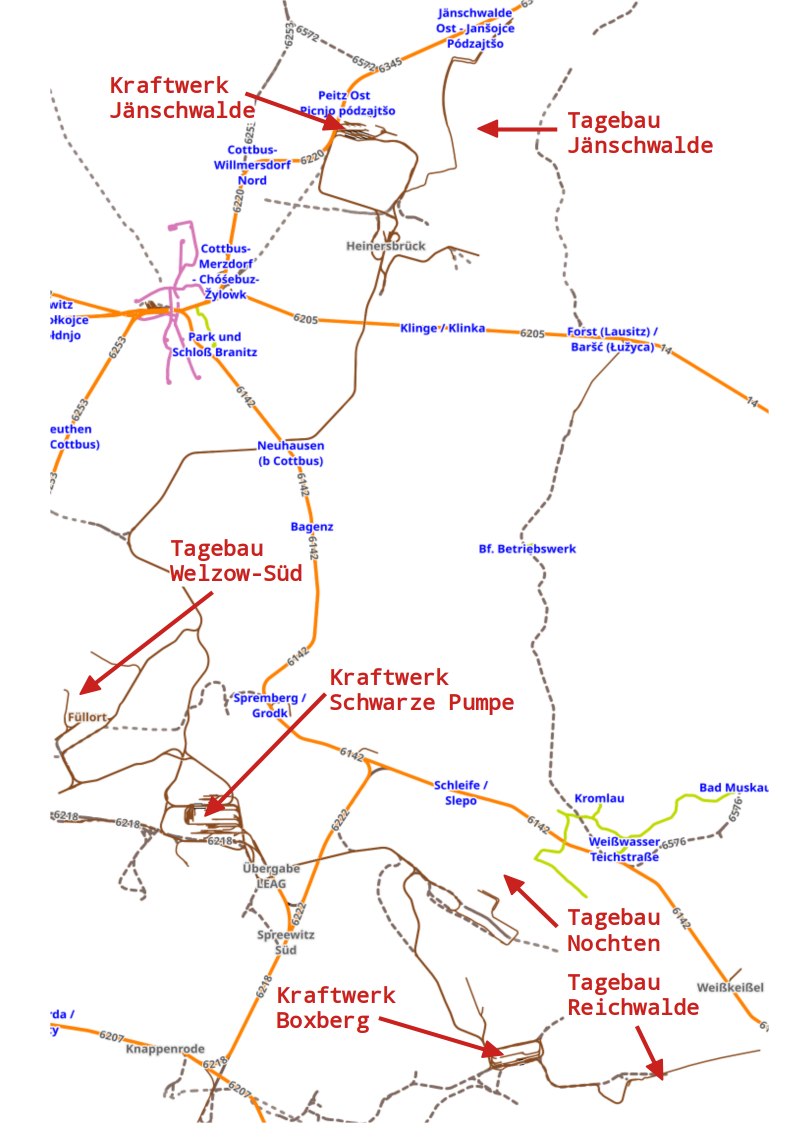
\includegraphics[width=0.75\linewidth]{images/LEAG-Netz-annotated.png}
	\caption{Das Schienennetz der LEAG für den Kohletransport (braun) und die Positionen der ansgeschlossenen Tagebaue und Kraftwerke (rot).}
	\label{fig:leag-netz}
\end{figure}
	\section{FlexiDug - Gemeinsam Nutzung durch Personen- und Güterzüge}

Nach dem Kohleausstieg würde das Potential des Schienennetzes ohne ein Nachnutzungskonzept ungenutzt bleiben \cite{rbb_hpi_2022}. Das Projekt \emph{FlexiDug} (Flexible, digitale Systeme für den schienengebundenen Verkehr in Wachstumsregionen) beschäftigt sich damit, Nachnutzungsperspektiven zu erstellen und ein solches Konzept bis zum Jahr 2024 zu erstellen \cite{hasso_plattner_institut_flexidug_2022}. Teil dieses Projektes sind die Analyse von Infrastrukturen, die Erstellung eines digitalen Zwillings des Schienennetzes, die Entwicklung von Sensornetzen zur Infrastrukturüberwachung und die Erforschung digitaler Leit- und Sicherungstechnik. All dies soll einen Personenverkehr auf diesem Schienennetz ermöglichen. Das große Ziel des Projektes ist das ''Ergründen von Perspektiven'' für die Nachnutzung der Infrastruktur und die Erforschung der Möglichkeit einer Nachnutzung, als auch einer gemeinsamen Nutzung durch Personen- und Güterzüge. \cite{rbb_hpi_2022} Diese Arbeit im Kontext des gesamten Softwareprojektes leistet einen Beitrag durch die Erweiterung des Verkehrssimulators \emph{SUMO}\footnote{\url{https://github.com/eclipse/sumo}} um ein realistischeres Modell des Zugverkehrs. Damit wird die Simulation von gleichzeitig fahrenden Personen- und Güterzügen auf dem Schienennetz der LEAG ermöglicht.
	\section{Das Softwareprojekt und die Interaktion im Team}

	\chapter{Grundlagen}
	\section{Fahrpläne}

Ein Fahrplan ist die zeitliche und räumliche Festlegung von Zugfahrten auf einem Schienennetz \cite{groger_simulation_2002}. Er enthält unter anderem
\begin{itemize}
    \item die Zuggattung,
    \item die Verkehrstage,
    \item die Strecke,
    \item die Ankunfts- Durchfahr- und Abfahrzeiten in allen Halte- und Betriebsstellen,
    \item und die zulässigen Geschwindigkeiten in den einzelnen Streckenabschnitten.
\end{itemize}
Der Fahrplan dient einer Reihe von Zwecken. Zum einen hilft der Fahrplan dabei, die vorhandene Infrastruktur auf die verkehrenden Züge zu verteilen und den Verkehr somit zu koordinieren. Damit können mögliche Konflikte bereits bei der Erstellung des Fahrplans lokalisiert werden. Weiterhin dient der Fahrplan als Informationsquelle für den Kunden und hilft diesem bei der Entscheidungsfindung bezüglich der Wahl der geeigneten Verkehrsmittel. Er dient den Triebfahrzeugführern und Fahrdienstleitern als Grundlage für ihre Betriebsplanung. Zusätzlich ermöglicht ein Fahrplan das Treffen von Aussagen für die Leistungsfähigkeit des Zugverkehrs. \cite{groger_simulation_2002}

	\section{Abfahrtspläne}

Zur Abgrenzung von dem Begriff Fahrplan wird hier der Begriff \emph{Abfahrtsplan} eingeführt. Im Gegensatz zu einem Fahrplan enthält ein Abfahrtsplan lediglich folgende Informationen:
\begin{itemize}
    \item Die Zuggattung (Im Folgenden Zugtyp genannt)
    \item Die Abfahrtszeiten an der Starthaltestelle
    \item Eine Liste der Zwischenhaltestellen und die Endhaltestelle jedoch keine Ankunfts- oder Abfahrtzeiten
\end{itemize}
Da die Ankunfts- und Abfahrtzeiten Teil der Ergebnisse sind, die die Simulation produziert, können Fahrpläne nicht als Eingabe dienen. Daher verwenden wir Abfahrtspläne. Wie bereits in den Anforderungen angedeutet, werde drei verschiedene Arten von Abfahrtsplänen benötigt. Solche die zeitlich regelmäßige Zugfahrten beschreiben (Regelmäßige Abfahrtspläne), solche die Zugfahrten mit zufälligen Abfahrtszeiten beschreiben (Zufällige Abfahrtspläne) und solche, deren Abfahrtzeiten sich nach einem historischen Kohlebedarf richten (Bedarfsorientierte Abfahrtspläne). Jeder Abfahrtsplan besitzt eine Startzeit $t_s \in \mathbb{N}$ und eine Endzeit $t_e \in \mathbb{N}$, jeweils in Sekunden. $t_s$ beschreibt den Zeitpunkt in der Simulation, wenn der Abfahrtsplan aktiv wird, $t_e$ beschreibt den Zeitpunkt, wenn der Abfahrtsplan deaktiviert wird. Für jede Abfahrtszeit eines Zuges $t_a$ gilt also $t_s\leq t_a \leq t_e$. Die Details der drei Varianten werden im Folgenden erklärt.

\subsection{Regelmäßige Abfahrtspläne}

Der regelmäßige Abfahrtsplan beschreibt die Abfahrt von Zügen in regelmäßigen zeitlichen Abständen und dient der Modellierung von klassischen fahrplan-basiertem Verhalten. Er besitzt eine Periode $p\in\mathbb{N}$ in Sekunden, welche die Größe des zeitlichen Abstandes angibt. Ein regelmäßiger Abfahrtsplan lässt somit Züge zu den Zeitpunkten $t_a=t_s+np$ mit $n\in\mathbb{N}$ abfahren.

\subsection{Zufällige Abfahrtspläne}

Der regelmäßige Abfahrtsplan beschreibt die Abfahrt von Zügen in zufälligen zeitlichen Abständen. Er dient damit der Modellierung von Zügen, die unplanmäßig oder unvorhergesehen kurzfristig fahren. Dieser Abfahrtsplan besitzt eine Wahrscheinlichkeitsverteilung $P$, die angibt, mit welcher Häufigkeit Züge in einer bestimmten Zeitspanne abfahren. $P$ folgt einer Gleichverteilung. Die Wahrscheinlichkeit für eine Abfahrt ist also zu jedem Zeitpunkt gleich.

\subsection{Bedarfsorientierte Abfahrtspläne}

Der bedarfsorientierte Abfahrtsplan beschreibt die Abfahrt von Zügen in zeitlichen Abständen, die sich nach einem historischen Kohlebedarf richten. Er dient damit der Modellierung von Kohlezügen. Dieser Abfahrtsplan besitzt eine Kohlebedarfsfunktion $k:\mathbb{N}\to\mathbb{R}$, die angibt, wie viel Kohle in Abhängigkeit von der Zeit $t$ benötigt wird. Sie ergibt sich aus den historischen Kohlebedarfsdaten. Weiterhin existieren der Zeitpunkt $t_0 \in \mathbb{N}$ in Sekunden, an welchem die historischen Daten beginnen und die Zeitspanne $t_r \in \mathbb{N}$ in Sekunden, welche die zeitliche Auflösung der Daten angibt. Weiterhin ist $c\in\mathbb{R}$ die Menge an Kohle, die ein Kohlezug transportieren kann. Zur Berechnung der Abfahrtszeiten wird zunächst die Funktion $a: \mathbb{N} \to \mathbb{R}$ aufgestellt, die den akkumulierten Kohlebedarf zum Zeitpunkt $t$ seit $t_0$ berechnet (siehe Formel \ref{eq:kohle-accu}). Dabei ist $n\in\mathbb{N}$ die Anzahl der Datenpunkte.

\begin{equation}
    a(t)=\sum_{i=0}^{n-1}  k(t_ri+t_0)\label{eq:kohle-accu}
\end{equation}

Der Abfahrtsplan soll nun stets dann Züge abfahren lassen, wenn die Menge an Kohle, die transportiert werden muss, die Menge erreicht, die ein Zug transportieren kann. Die transportierte Menge wird dann von der bisher akkumulierten Menge abgezogen. Formel \ref{eq:kohle-fmod} stellt das dar.

\begin{equation}
    f(t, c)=fmod(a(t), c)\label{eq:kohle-fmod}
\end{equation}\footnote{Die Funktion $fmod:(\mathbb{R},\mathbb{R}) \to \mathbb{R}$ ist definiert als $(x,y)\mapsto x-ny$ mit $n\in\mathbb{Z}$, $x<0\Leftrightarrow fmod(x,y)<0$ und $fmod(x,y)<|y|$. Intuitiv formuliert, gibt die Funktion den Rest der Division $\frac{x}{y}$ zurück.}

Abbildung \ref{fig:demand-math} zeigt schematisch das Verhalten eines bedarfsorientierten Abfahrtsplans. $k(t)$ zeigt den (hier zur Vereinfachung konstanten) Kohlebedarf. $a(t)$ stellt den akkumulierten Kohlebedarf dar. $f(t,c)$ zeigt die akkumulierte Kohlemenge abzüglich der transportierten Kohlemenge. Die Abfahrtszeiten sind durch rote Pfeile markiert.

\begin{figure}[H]
	\centering
	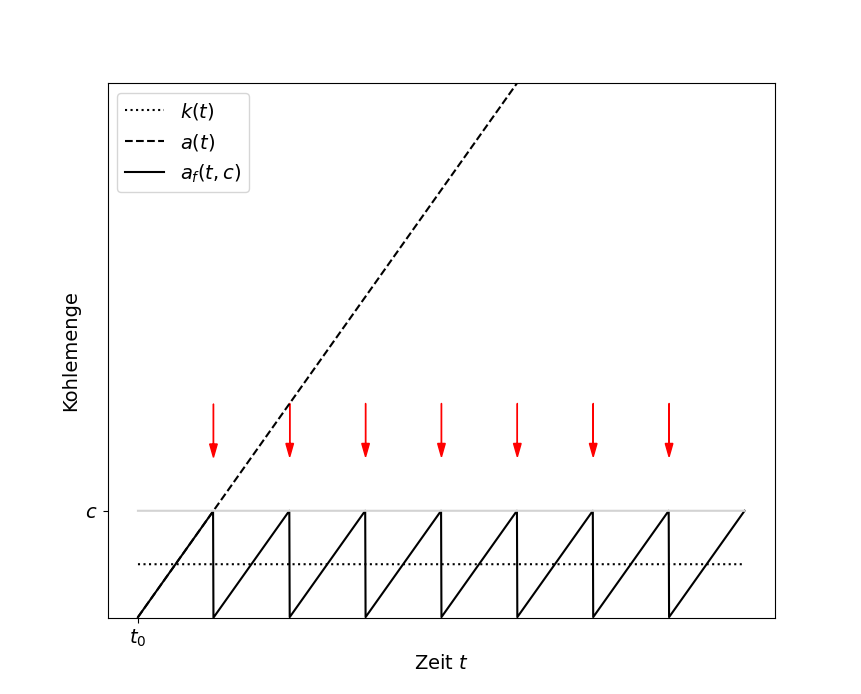
\includegraphics[width=1.0\linewidth]{images/demand-math.png}
	\caption{Schematisches Verhalten eines bedarfsorientierten Abfahrtsplans mit dem Kohlebedarf $k(t)$, dem akkumulierten Kohlebedarf $a(t)$ und der akkumulierten Kohlemenge abzüglich der transportierten Kohlemenge $f(t,c)$. Die roten Pfeile markieren die Abfahrtszeiten der Kohlezüge.}
	\label{fig:demand-math}
\end{figure}
	\section{Entwurfsmuster}

Nach dem Architekten Christopher Alexander lässt sich ein Entwurfsmuster\footnote{auch engl. \emph{Design Pattern}} folgendermaßen beschreiben:

\blockquote{Each pattern describes a problem which occurs over and over again in our environment, and then describes the core of the solution to that problem, in such a way that you can use this solution a million times over, without ever doing it the same way twice.} \cite{gamma_design_1995}

Obwohl diese Aussage auf Gebäude bezogen war, lässt sie sich ebenso gut auch Softwarearchitekturen anwenden. Auch in der Planung großer Softwaresysteme treten häufig dieselben abstrakten Probleme auf, welche sich mit einer Menge von Entwurfsmusters lösen lassen, welche die Beziehungen und Interaktionen von Objekten spezifizieren.

Ein Entwurfsmuster besteht dabei immer aus vier Elementen, seinem Namen, einer Problembeschreibung, einer Lösung und den sich ergebenden Konsequenzen \cite{gamma_design_1995}. Die Problembeschreibung gibt dabei an, in welchen Fällen sich ein Muster anwenden lässt, während die Lösung die Beziehungen und Verantwortlichkeiten der beteiligten Objekte beschreibt. Sie geht dabei nicht auf individuelle Anwendungsfälle ein, sondern stellt lediglich eine abstrakte Herangehensweise an das Problem bereit. Jedes Muster bringt Vor- und Nachteile mit sich und geht Kompromisse zwischen verschiedenen Qualitätsaspekten ein. Die Konsequenzen beleuchten diese und helfen bei der Argumentation für oder gegen eine konkrete Designentscheidung.

Im Folgenden werden die abstrakten Entwurfsmusters beschrieben, welche in der Architekturdiskussion eine Rolle spielen werden.

\subsection{Strategy Pattern}
\subsection{Template Method}

\subsubsection*{Problembeschreibung}

Es existieren ein Algorithmus, welcher aus einer Menge von Teilschritten besteht. Die einzelnen Teilschritte sollen austauschbar gehalten werden, um ein flexibles Anpassen des Algorithmus zu ermöglichen. Die Reihenfolge der Teilschritte ist hingegen festgelegt. 

\subsubsection*{Lösung}

\begin{figure}[!hb]
	\centering
	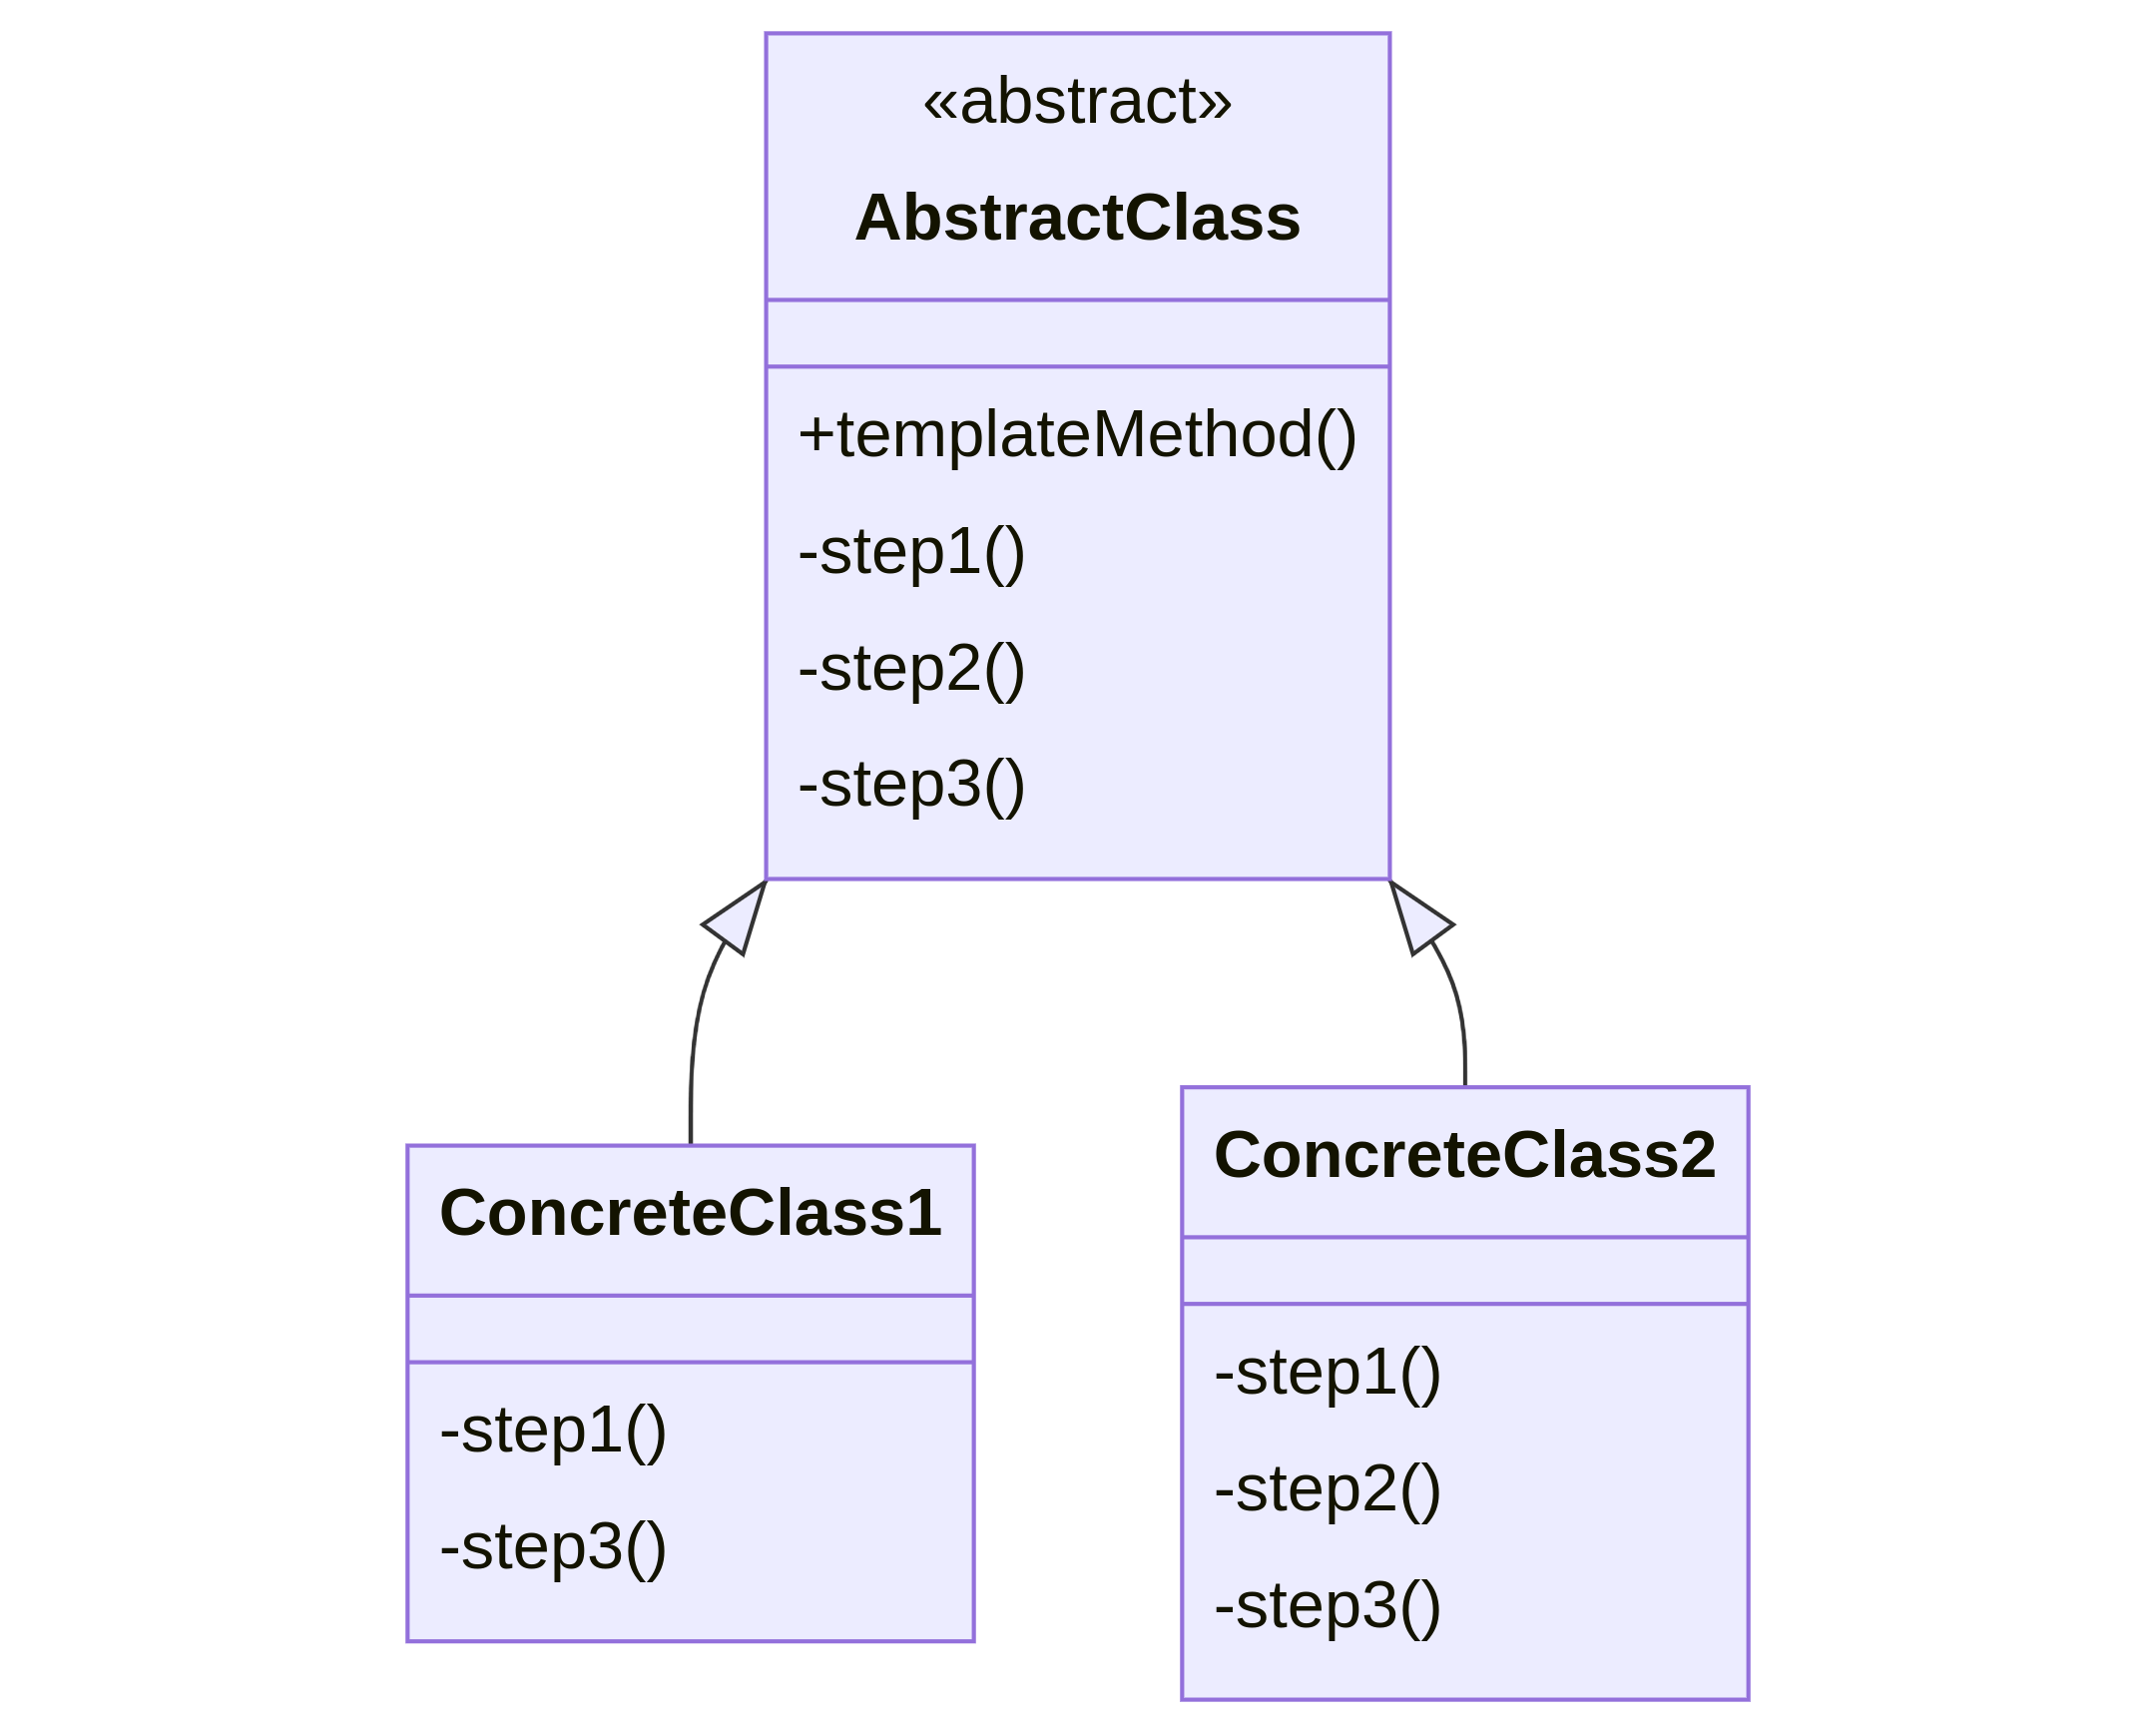
\includegraphics[width=0.75\linewidth]{images/patterns/template-method-class.png}
	\caption{Klassendiagramm Template Method}
	\label{fig:template-method-class}
\end{figure}

Jede Klasse, welche einen Algorithmus der selben Struktur implementiert, erbt von einer abstrakten Klassen, welche die `templateMethod` implementiert. Diese gibt das Grundgerüst des Algorithmus vor und ruft darin die einzelnen Teilschritte auf. Diese sind jeweils in eigenen Methoden implementiert. Die Subklassen definieren diese Methoden zum Teil neu, wenn eine Veränderung des Verhaltens dieses Teilschrittes notwendig ist.


\lstset{language=python}
\begin{lstlisting}[caption={Quelltextunterschrift}, label=code:template-method-code]
class AbstractClass:
	def templateMethod(self):
    	if self.step1():
        	self.step2()
    	self.step3()
\end{lstlisting}


\subsubsection*{Konsequenzen}

Template Methods sind ein Mechanismus, welcher die Wiederverwendung von Code ermöglicht und kann somit der Codeduplikation entgegen wirken. Anstatt Abwandlungen von Algorithmen von Grund auf neu zu implementieren, ist es möglich, sie aus bestehenden Komponenten zusammenzusetzen und je nach Bedarf neuen Code hinzuzufügen. Das Muster der Template-Method weist eine umgekehrte Kontrollstruktur auf. Anstatt dass eine Klasse Methoden ihrer Superklasse aufruft, delegiert die Template-Method die Verantwortlichkeit für die einzelnen Teile des Algorithmus an sie Subklassen.

Bei der Verwendung der Template-Method ist jedoch zu beachten, wie die einzelnen Methoden zu verwenden sind. Diese lassen sich grob in zwei Arten einteilen, Die "Hook"-Methoden und die abstrakten Methoden. Während die "Hook"-Methoden eine Standard-Implementierung in der abstrakten Basisklasse bereitstellen, ist dies bei den abstrakten Methoden nicht der Fall. Entsprechend müssen die abstrakten Methoden zwingend von einer konkreten Subklasse implementiert werden. Bei den "Hook"-Methoden ist das optional. 

Die Template-Method synergiert mit dem Strategy-Pattern. Einzelne Schritte eine Algorithmus können in einer Strategie-Klasse implementiert sein.
\subsection{Observer Pattern}


\subsubsection*{Problembeschreibung}

Häufig müssen verschiedene Komponenten eines Systems synchron gehalten werden. Gleichzeitig soll aber auch eine enge Kopplung dieser Komponenten vermieden werden. Es wird eine $1$:$n$-Beziehung zwischen den Objekten benötigt, wobei $n$ Objekte von einem Objekt abhängen. Wenn das eine Objekt seinen Zustand ändert, so sollen alle abhängigen Objekte benachrichtigt werden, sodass auch sie ihren Zustand aktualisieren können. Ein naiver Lösungsansatz wäre, jedem abhängigen Objekt eine Referenz auf das Objekt zu geben, von welchem es abhängt. Die Objekte könnten dann in regelmäßigen Abständen prüfen, ob eine Zustandsänderung stattgefunden hat (\emph{Polling}). Dieser Ansatz weist jedoch nicht nur eine hohe Kopplung auf, er ist auch wenig performant. Auch wenn keine Zustandsänderung stattgefunden hat, wird auf diese geprüft. Der Aufwand für diese Prüfung steigt dabei linear mit der Anzahl der beteiligten Objekte.

Das \emph{Observer-Pattern} kann Anwendung finden, wenn es zwei voneinander getrennte Konzepte gibt und eines von dem anderen abhängig ist. Die Abhängigkeit kann modelliert werden, ohne die Objekte stark zu koppeln. Weiterhin ist es möglich, die Anzahl der abhängigen Objekte variablen zu halten. \cite{gamma_design_1995}

\subsubsection*{Lösung}

Das Observer-Pattern besteht aus einem Sender (\code{Publisher}) und mehreren Empfängern (\code{ConcreteSubscriber}). Die Empfänger implementieren die Empfänger-Schnittstelle (\code{Subscriber}), welches eine Methode \code{update} zur Aktualisierung des Zustandes bereitstellt. Der Sender hält eine Liste von Referenzen auf Empfänger und verfügt über die Methoden \code{subscribe} und \code{unsubscribe}, welche es ermöglichen, der Liste Empfänger hinzuzufügen, oder sie zu entfernen (siehe Abbildung \ref{fig:observer-class}).

\begin{figure}[htb]
	\centering
	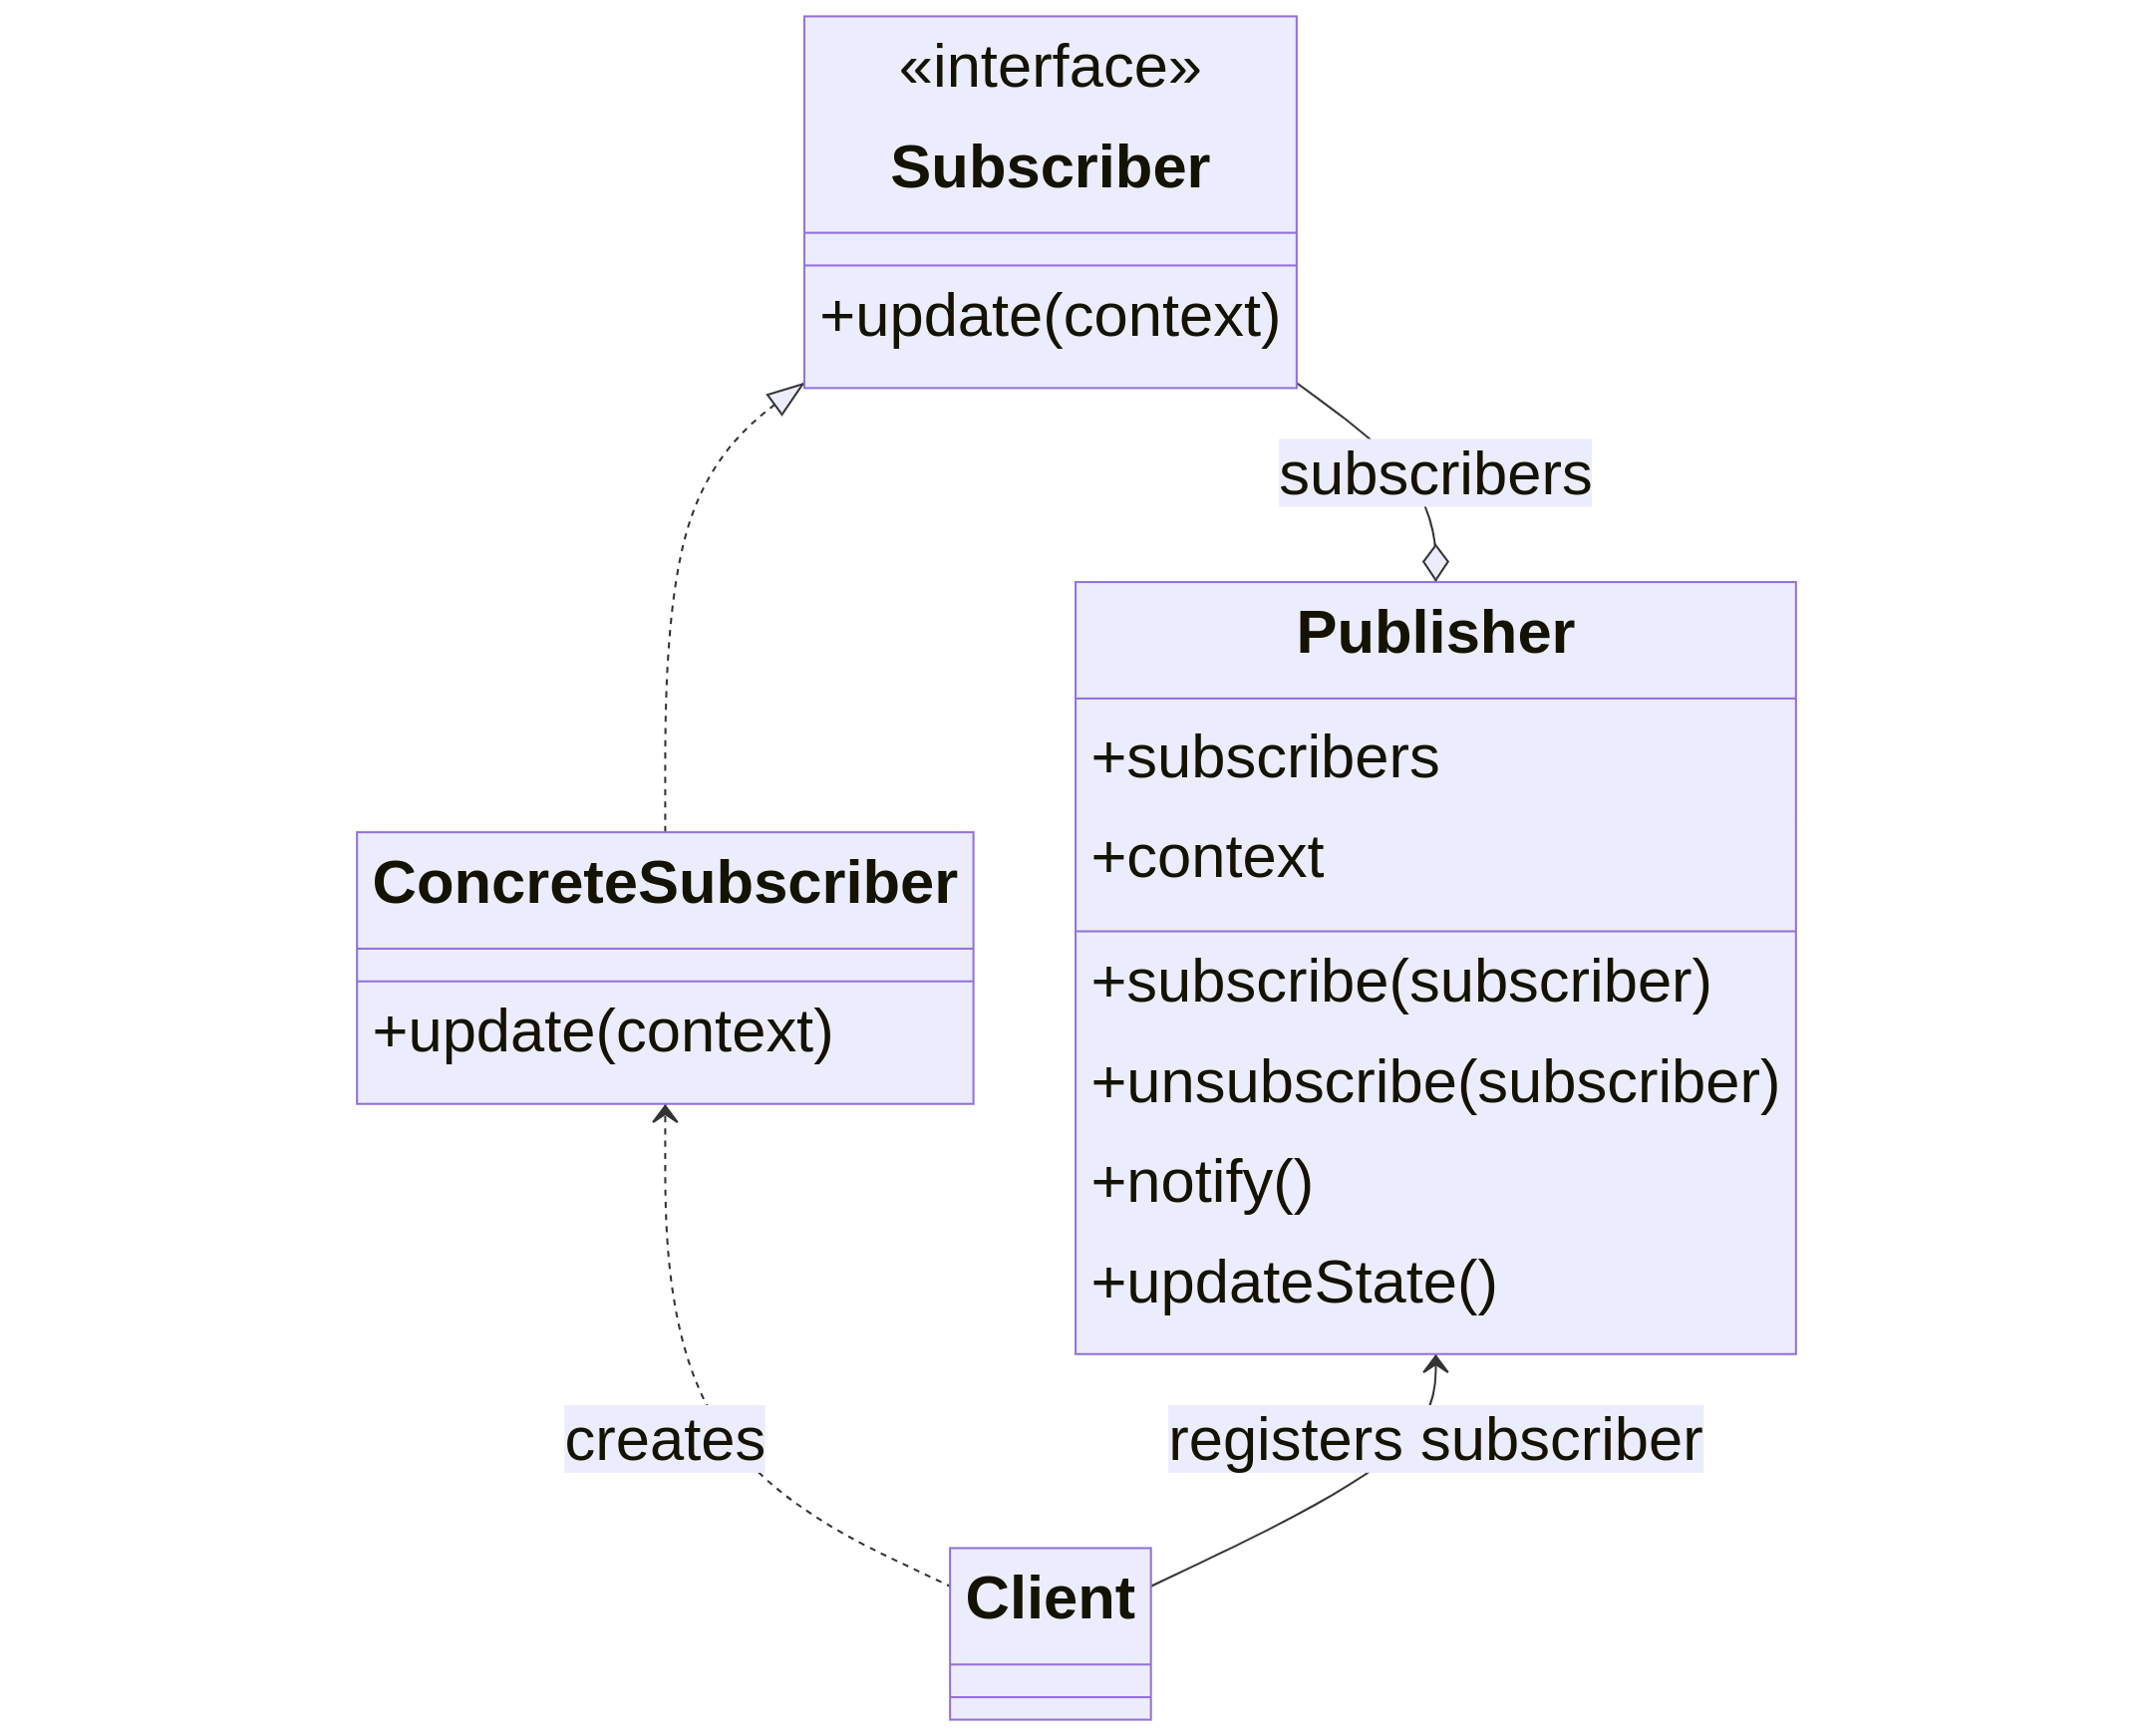
\includegraphics[width=0.95\linewidth]{images/patterns/observer-class.png}
	\caption{Klassendiagramm des Observer-Patterns \cite{skobeleva_observer_2023}}
	\label{fig:observer-class}
\end{figure}

Abbildung \ref{fig:observer-seq} zeigt, dass der Anwender (\code{Client})\footnote{Der Anwender (\code{Client}) ist in der Regel eine weitere Klasse, welche den beschriebenen Mechanismus verwendet. Es handelt sich in aller Regel nicht um einen Meenschen.} den Zustand des Sender durch Senden von \code{updateSate} verändern kann (1). Der Sender sendet sich draufhin selbst \code{notify} (2) und beginnt über seine Liste von Empfängern zu iterieren. Jedem Empfänger sendet er dann \code{update} (3, 5) und übergibt den notwendigen Kontext, sodass der Empfänger seinen Zustand entsprechend aktualisieren kann.

\begin{figure}[htb]
	\centering
	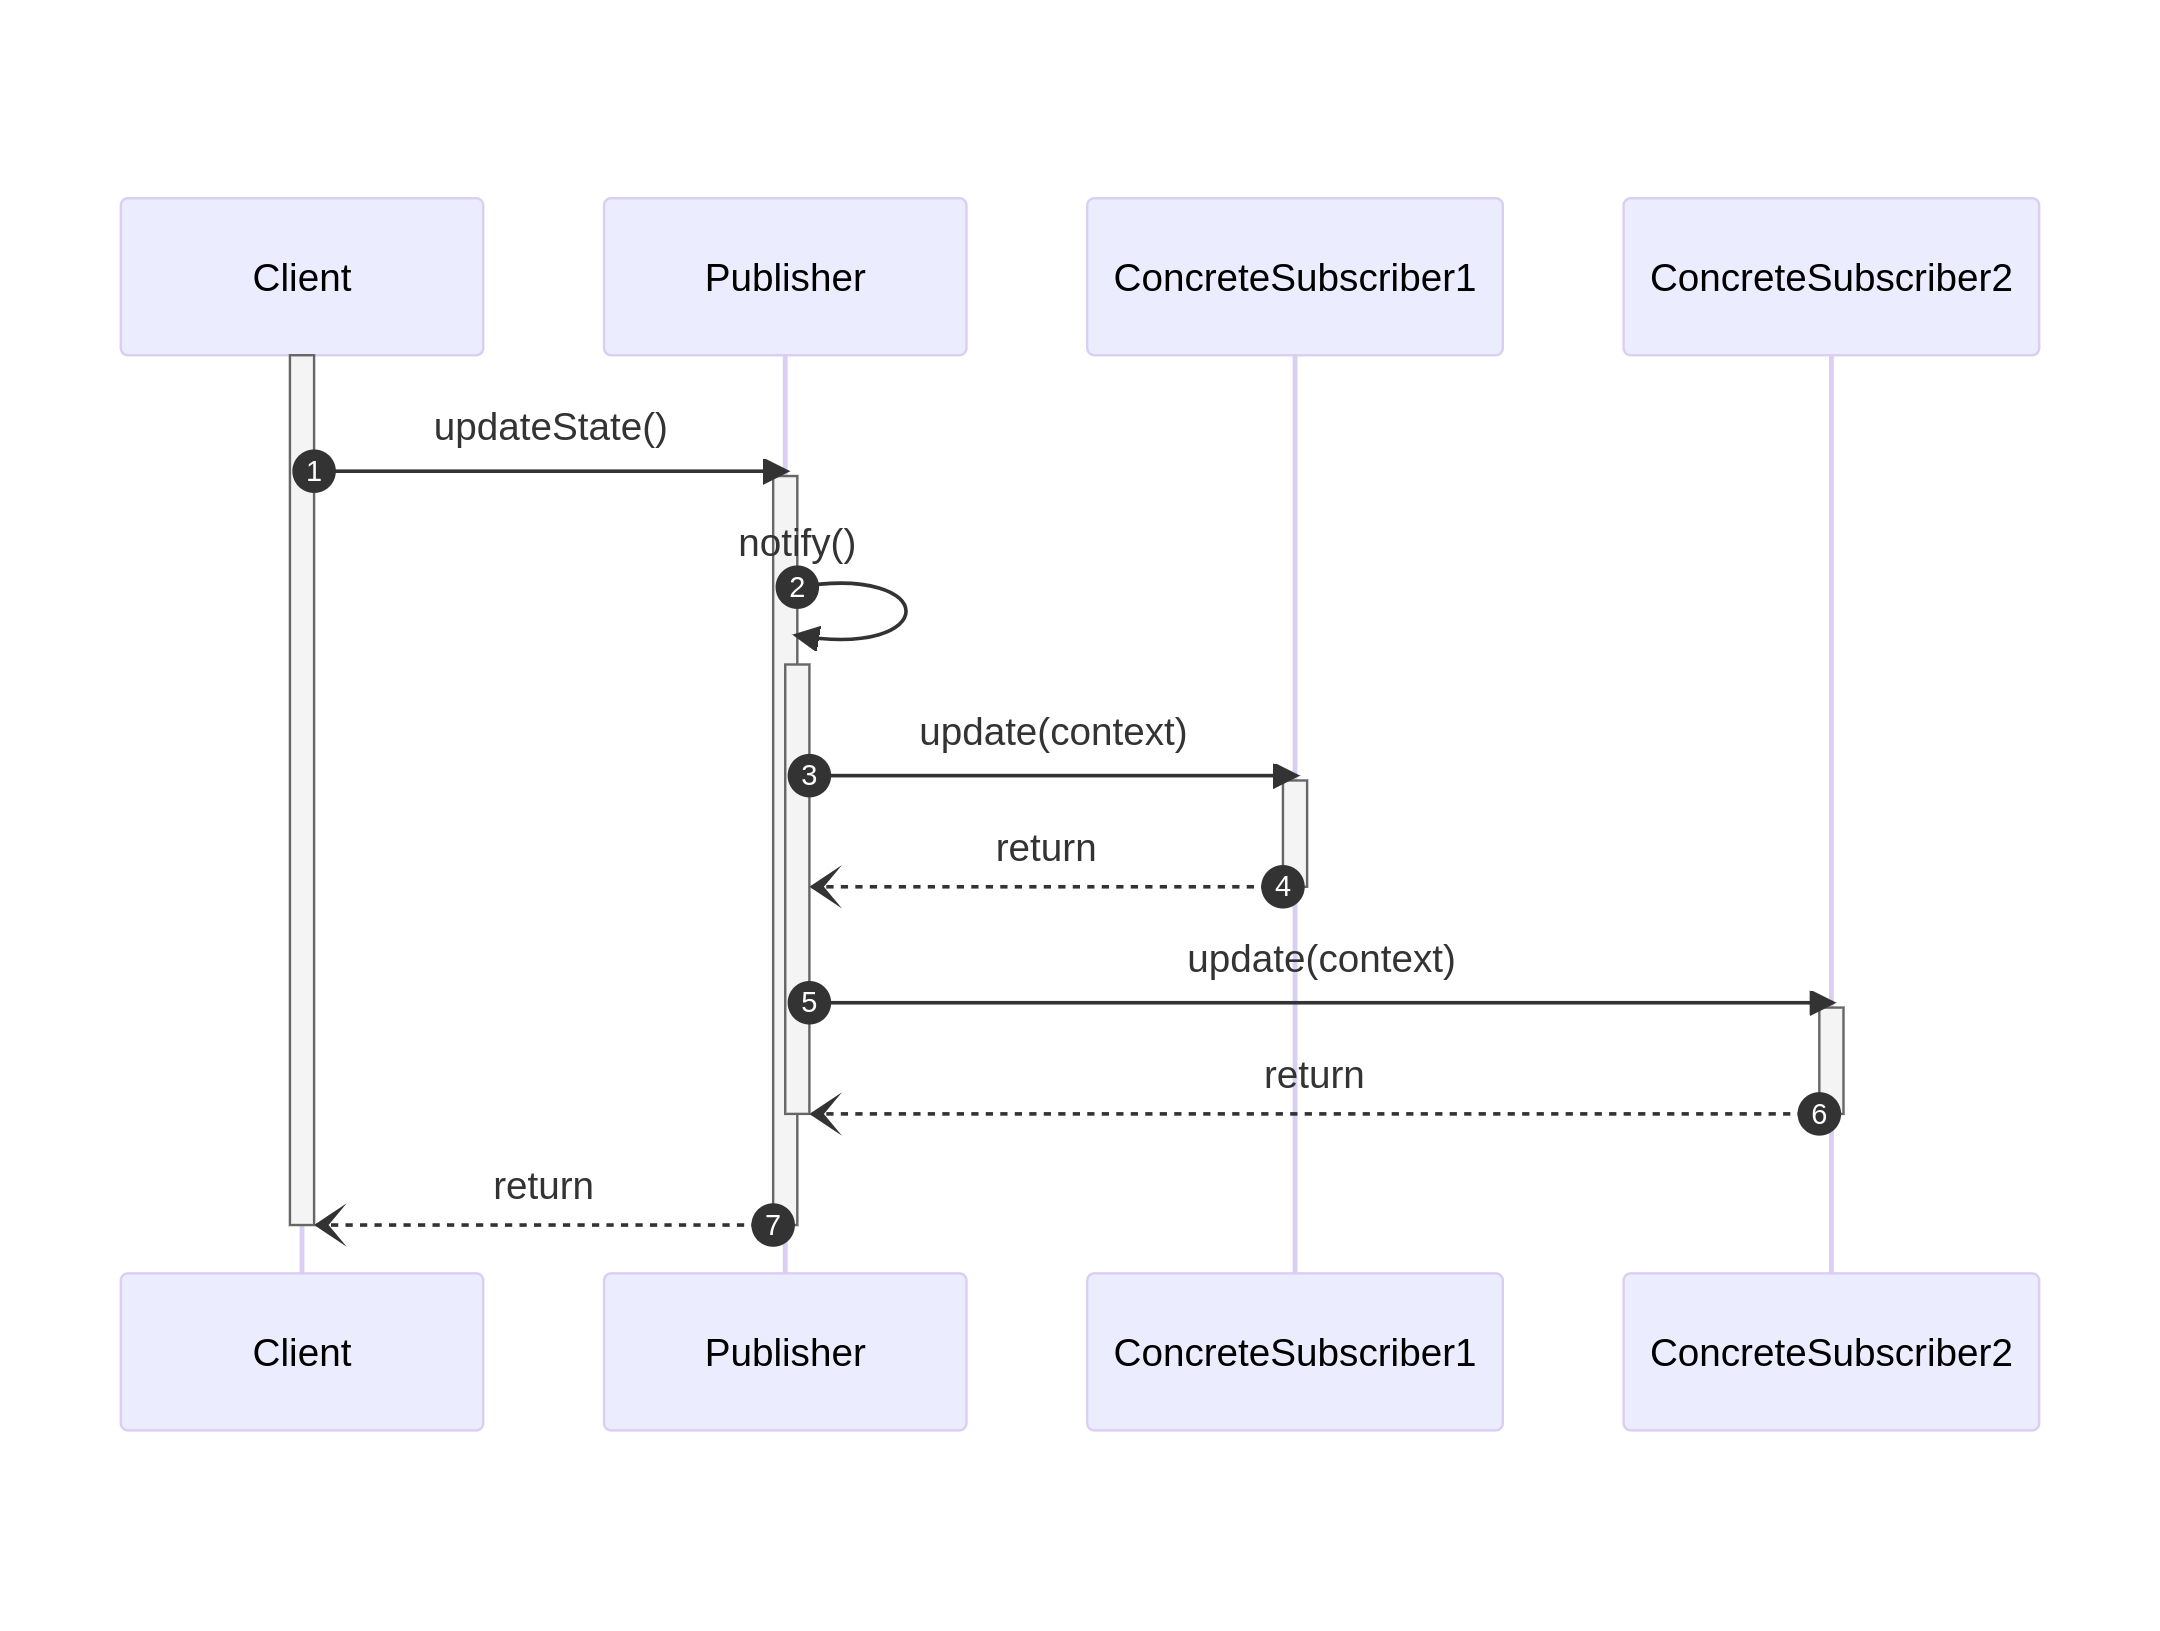
\includegraphics[width=0.95\linewidth]{images/patterns/observer-seq.png}
	\caption{Sequenzdiagramm des Observer-Patterns \cite{skobeleva_observer_2023}}
	\label{fig:observer-seq}
\end{figure}

Quelltext \ref{code:observer-code} veranschaulicht die Benachrichtigung aller Empfänger. In \code{notify} wird an jeden im Sender referenzierten Empfänger \code{update} gesendet. Dabei wird der Kontext des Senders an jeden Empfänger übergeben.

\lstset{language=python}
\begin{lstlisting}[caption={Quelltext der Methode \code{notify} des Publishers, welche über alle Empfänger iteriert und diese benachrichtigt.}, label=code:observer-code]
class Publisher
	def notify(self):
        for subscriber in self.subscribers:
            subscriber.update(self.context)
\end{lstlisting}


\subsubsection*{Konsequenzen}

Das Observer-Pattern bietet eine Reihe von Vorteilen. Durch Separation von Sender und Empfänger und durch die Abstraktion der Empfänger-Schnittstelle wird eine lose Kopplung der beiden erreicht. Diese lose Kopplung ermöglicht es, sowohl den Sender, als auch die Empfänger beliebig auszutauschen. Weiterhin können sich der Sender und die Empfänger auf unterschiedlichen Abstraktionsniveaus befinden. Ein Sender auf einem niedrigen Level kann einen Empfänger auf einem hohen Level benachrichtigen. Wären Empfänger und Sender nicht getrennt, so wäre dafür ein Abstraktionshierarchie-übergreifendes Objekt notwendig, welches die Trennung der Abstraktionsschichten beeinträchtigen würde. Ein weiterer Vorteil ist die dynamische Anzahl der Empfänger, mit denen ein Sender interagieren kann. So kann der Anwender über den Sender eine beliebige Zahl an Empfängern erreichen.

Ein Nachteil des Observer-Patterns ist, dass der Sender stets alle seine Empfänger benachrichtigt. Es kann vorkommen, dass nur eine Teilmenge der Empfänger die Benachrichtigung benötigt, was in unnötigen Methodenaufrufen resultiert. \cite{gamma_design_1995}
\subsection{Mediator Pattern}


\subsubsection*{Problembeschreibung}

Große Softwareprojekte bestehen meist aus einer einer enormen Anzahl an Klassen bzw. Objekten, welche miteinander interagieren. Ziel ist es stets, die Kopplung zwischen diesen Komponenten so gering wie möglich zu halten. Komplexe Interaktionsmuster zwischen diesen Objekten lassen sich nicht immer verhindern, das sie die inhärente Komplexität des modellierten Problems wiederspiegeln. In diesem Fall ist eine Lösung notwending, die diese Komplexität kapselt. Das Mediator-Pattern ist in der Lage, solche Fälle von komplexer Interaktion zu vereinfachen.

\subsubsection*{Lösung}

Der konkrete Mediator implementiert das Mediator-Interface, welches eine Methode `notify` bereitstellt, um Benachrichtigungen der einzelnen Komponenten entgegenzunehmen. Jede Komponente besitzt eine Referenz auf den Mediator, um `notify`an ihn senden zu können. Dabei übergibt die Komponente sich selbst, um dem Mediator den Kontext der Benachrichtigung bereitzustellen. In Abhängigkeit des übergebenen Senders und dessen Zustand, führt der Mediator eine (komplexe) Logik aus, welche vollständig innerhalb des Mediators gekapselt ist. Der Mediator hält ebenso Referenzen auf alle Komponenten, die er zu beeinflussen in der Lage sein soll. Die gekapselte Logik kann somit die Interfaces der Komponenten verwenden, um diese zu beeinflussen. Dadurch findet eine indirekte Beeinflussung von Komponenten durch andere Komponenten über den Mediator statt.  

\begin{figure}[!hb]
	\centering
	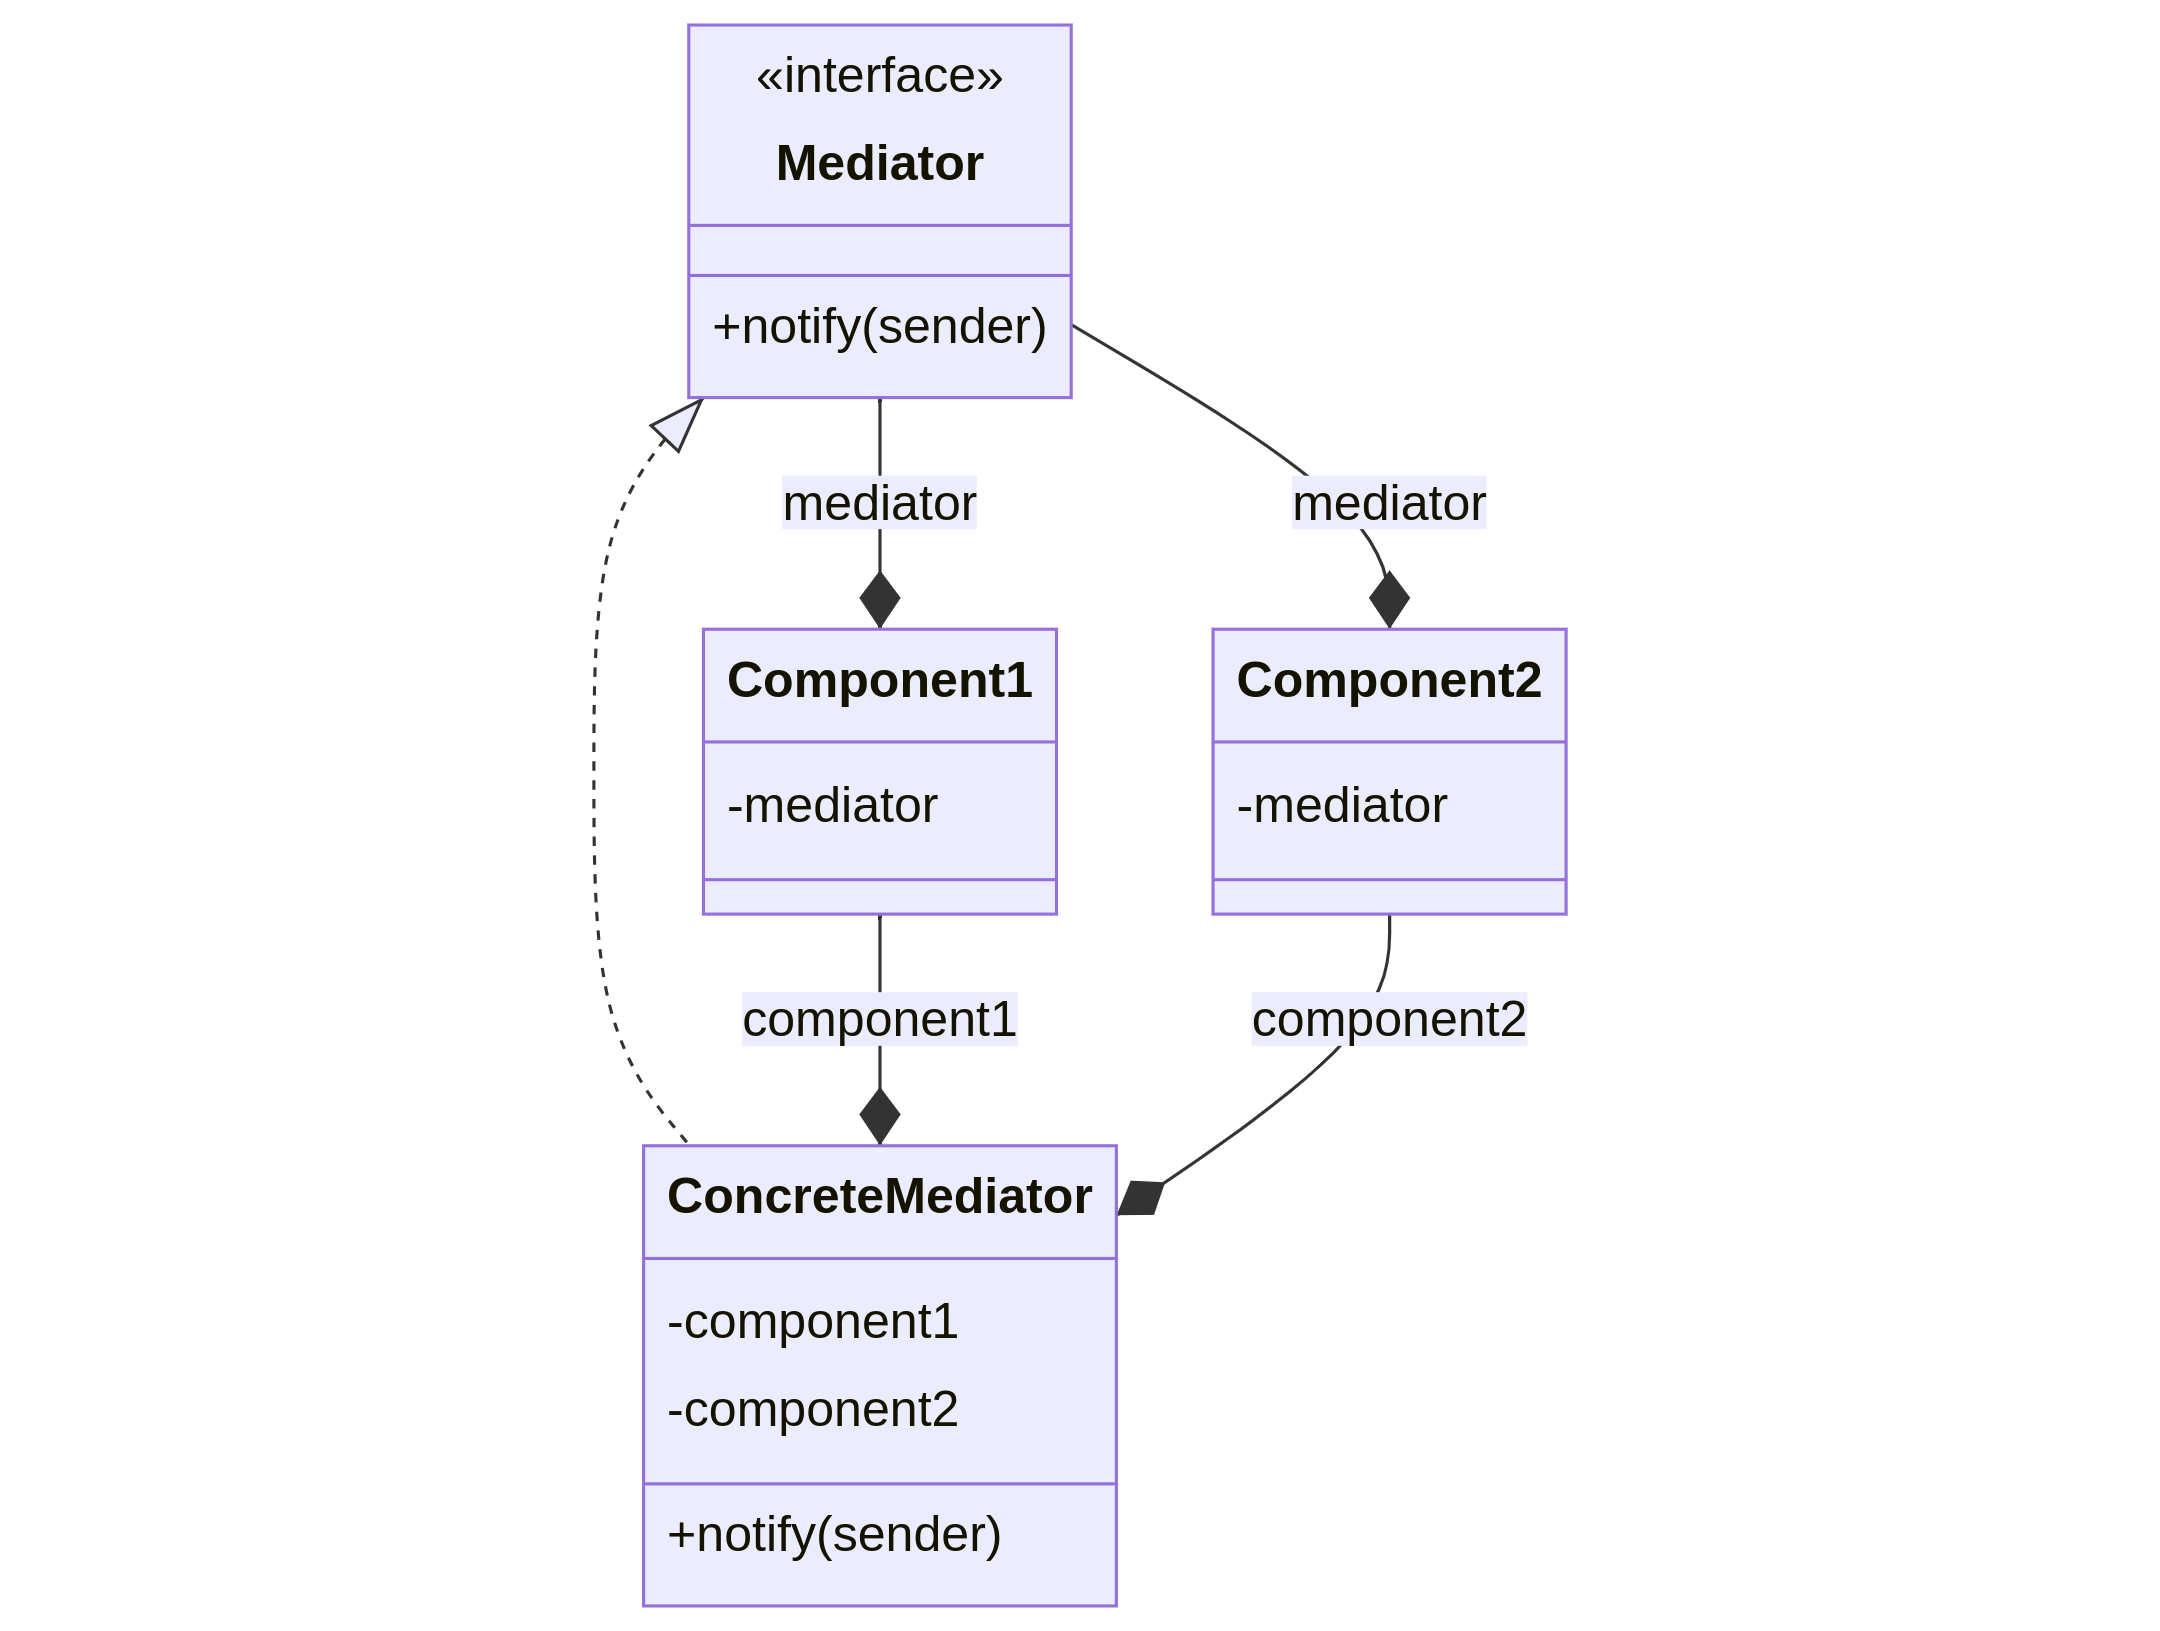
\includegraphics[width=0.75\linewidth]{images/patterns/mediator-class.png}
	\caption{Klassendiagramm Mediator Pattern}
	\label{fig:mediator-class}
\end{figure}

\subsubsection*{Konsequenzen}

Der Mediator kapselt Verhalten, welches ansonsten über mehrere Klassen verteilt wäre. Soll dieses Verhalten spezialisiert werden, so ist nur eine Spezialisierung des Mediators notwendig. Weiterhin verhindert der Mediator eine starke Kopplung der Komponenten. Komponenten- und Mediator-Klassen können bei kompatiblen Interfaces beliebig ausgetauscht werden. Der Mediator vereinfacht außerdem die Multiplizitäten von Objektinteraktionen. Er wandelt $m$:$n$- Beziehungen zwischen Objekten in $1$:$n$-Beziehungen zwischen den Objekten und dem Mediator um. 

Der Mediator bündelt Kontrolle an einem einzigen Punkt. Dies kann zur Übersichtlichkeit beitragen, kann dieser jedoch bei ausreichend komplexer Logik entgegenwirken. Das kann dem Mediator eine monolithische Struktur geben, deren Verhinderung seine eigentliche Aufgabe ist. 

Sind die Abhängigkeiten zwischen den Komponenten zu Komplex, so kann das Observer-Pattern zur Kommunikation zwischen den Komponenten und dem Mediator verwendet werden. Dadurch lassen sich die Abhängigkeiten außerdem flexibler gestalten, sie können also zur Laufzeit einfacher geändert werden.
\subsection{\emph{Visitor-Pattern} und \emph{Double Dispatch}}


\subsubsection*{Problembeschreibung}

Gelegentlich muss eine Operation auf einer Menge von Objekten durchgeführt, die alle Teil einer Objekthiearchie aber unterschiedlich sind. Diese Objekte besitzen daher unter Umständen voneinander abweichende Interfaces. Das \emph{Visitor-Pattern} erlaubt es, solche Operationen außerhalb der Objekte und für alle betroffenen Objekte innerhalb einer separaten Klasse zu definieren. \cite{gamma_design_1995}

\subsubsection*{Lösung}

Der konkrete \emph{Visitor}\footnote{Die deutsche Übersetzung ''Besucher'' ist in diesem Kontext eher unüblich.} (\code{ConcreteVisitor}) realisiert die \emph{Visitor}-Schnittstelle (\code{Visitor}), welche die Methode \code{visit} bereitstellt, wie in Abbildung \ref{fig:visitor-class} zu erkennen ist. Diese erlaubt es dem \emph{Visitor}, ein Element (\code{Element}) zu ''besuchen'' und auf ihm eine Operation durchzuführen. Die Elemente ''akzeptieren'' den ''Besuch'' des \emph{Visitors} mit Hilfe der Methode \code{accept}, welche als Argument den besuchenden\emph{Visitor} erhält.

\begin{figure}[H]
	\centering
	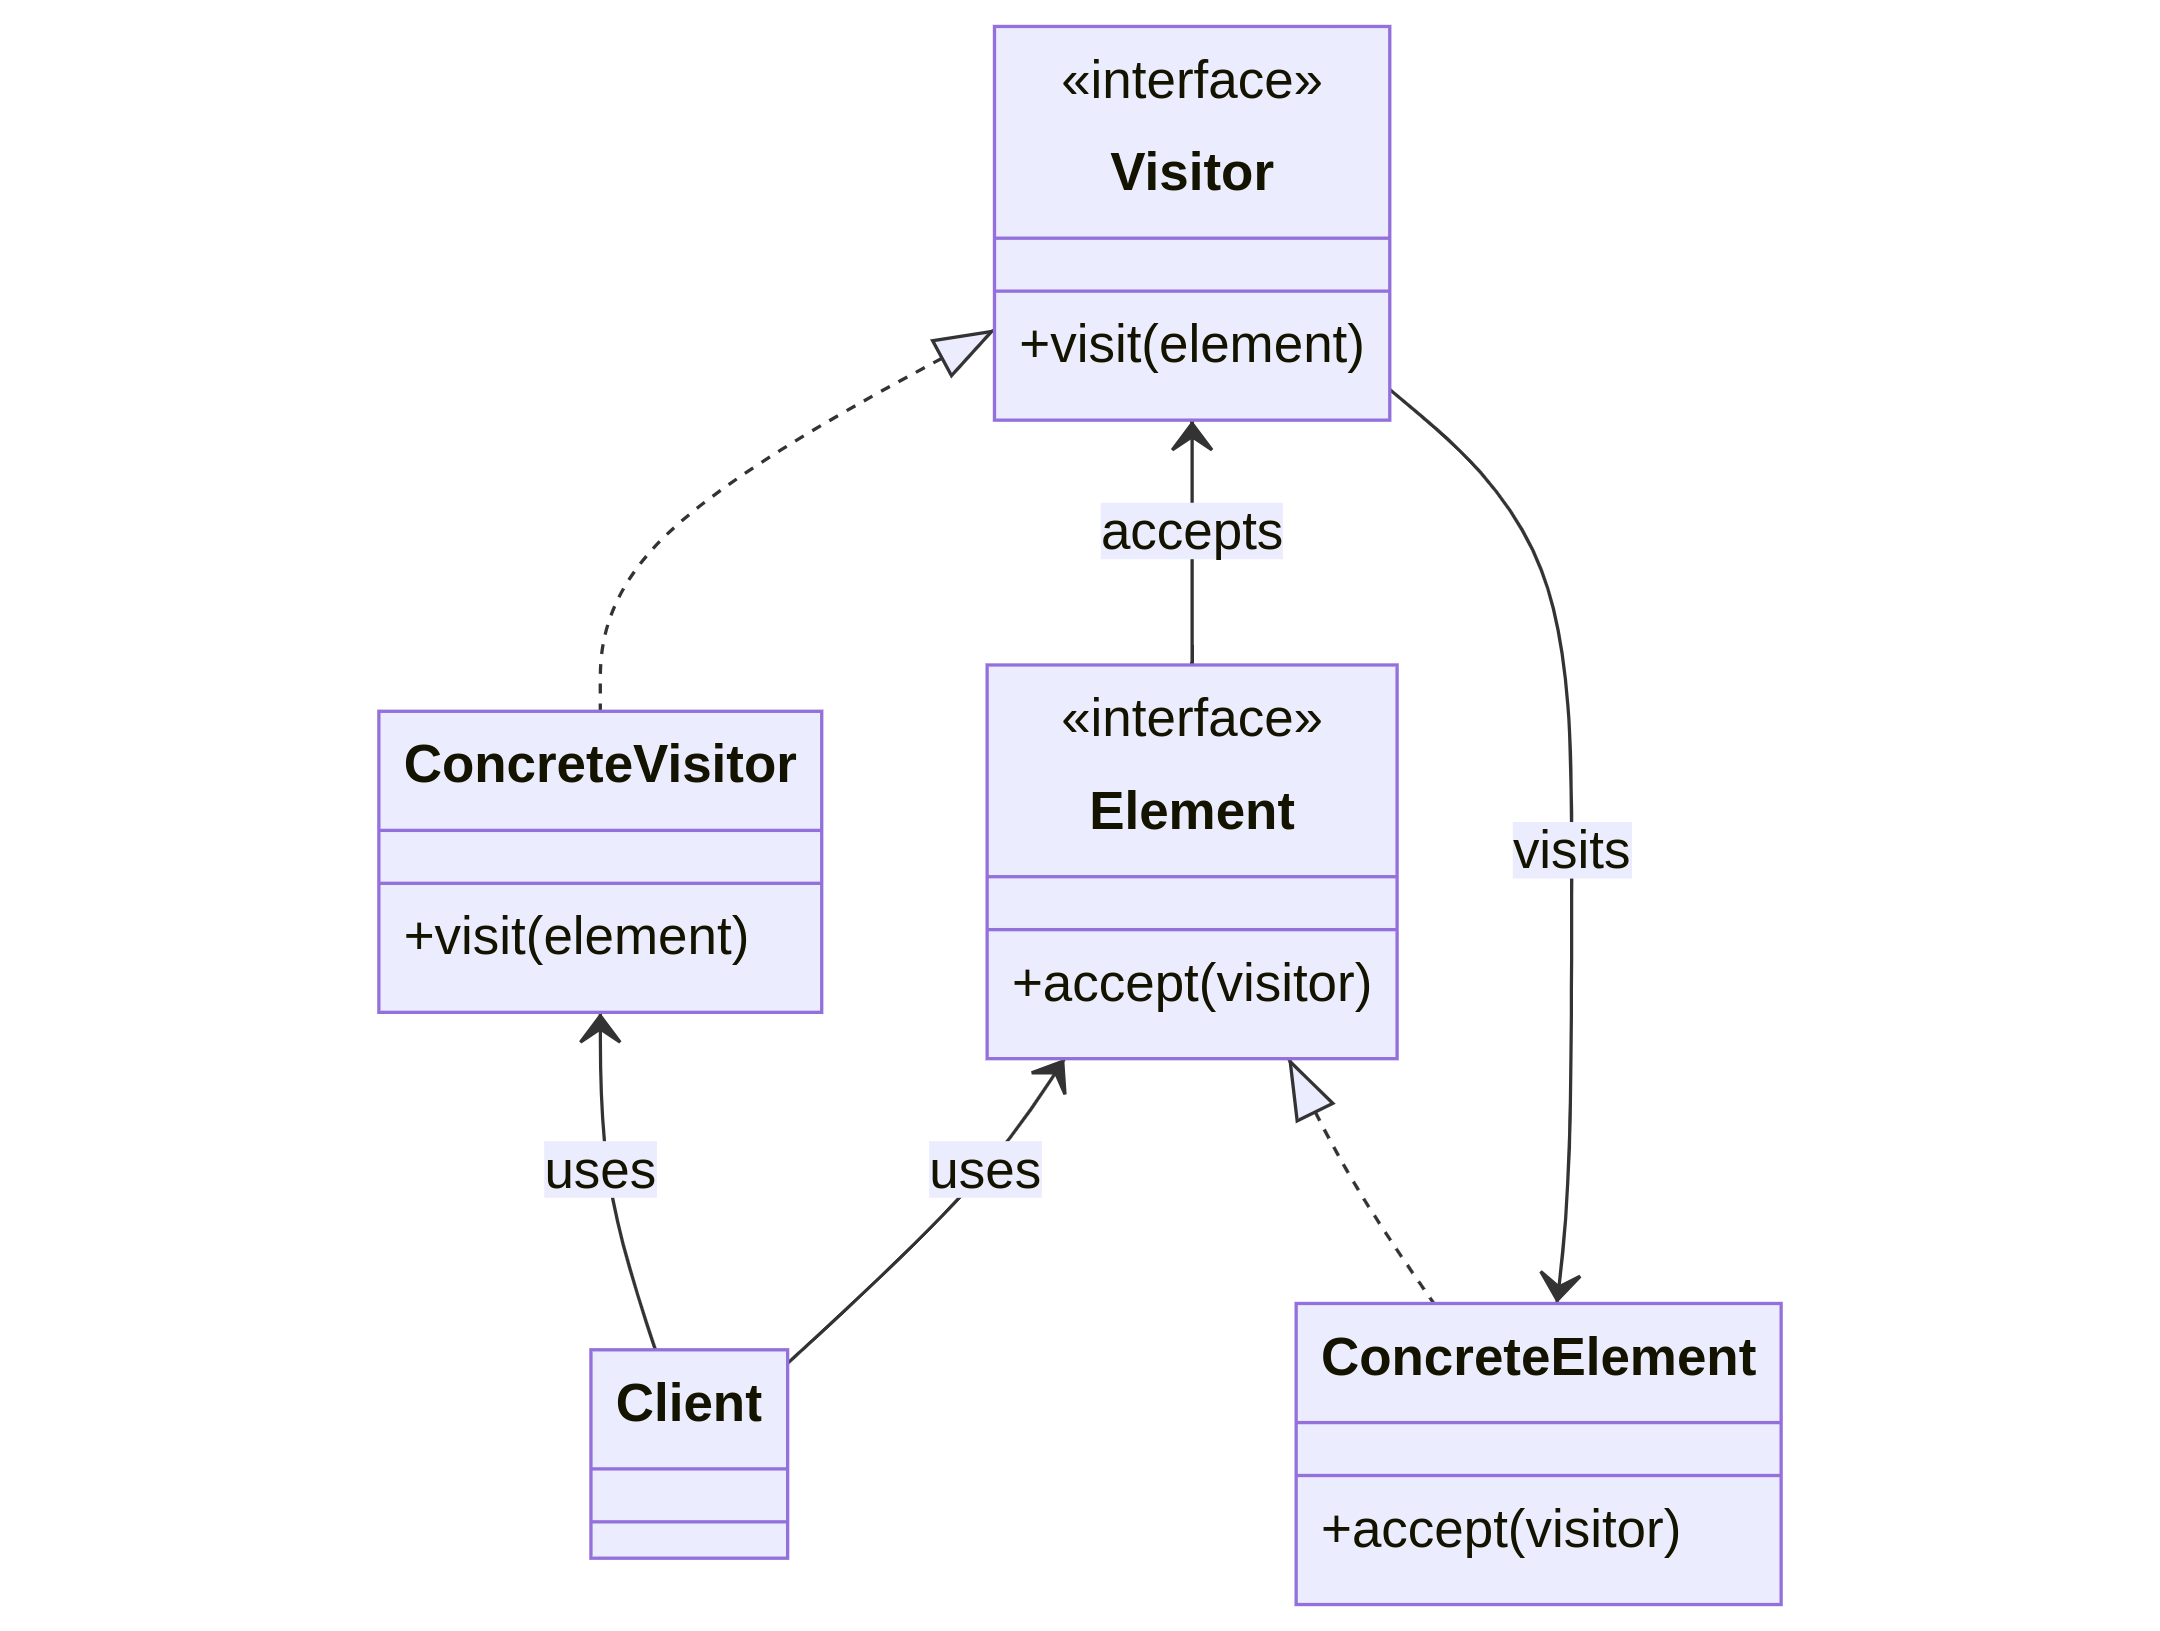
\includegraphics[width=0.75\linewidth]{images/patterns/visitor-class.png}
	\caption{Klassendiagramm des \emph{Visitor-Patterns}. \cite{skobeleva_visitor_2023}}
	\label{fig:visitor-class}
\end{figure}

Abbildung \ref{fig:visitor-seq} zeigt das Verhalten des \emph{Visitor-Patterns}. Der Anwender\footref{ftn:client} trägt dem\emph{Visitor} auf, eine Operation auf einem Element oder einer Menge von Elementen durchzuführen (1). Der\emph{Visitor} sendet daraufhin \code{visit} an alle Elemente, auf die er eine Referenz hält (2). Jedes Element ruft daraufhin eine \code{accept}-Methode auf dem\emph{Visitor} auf (3). Zu beachten ist hierbei, dass es für jede Element-Klasse eine eigene Methode im\emph{Visitor} gibt. Dies kann realisiert werden durch das Bereitstellen von Methoden mit unterschiedlichen, zu den aufrufenden Klassen korrespondierenden Namen oder durch Multimethoden. Multimethoden sind Methoden, welche je nach Typ der übergebenen Argumente unterschiedliche Implementierungen ausführen. Somit kann der\emph{Visitor} nach Erhalt von \code{accept} die zum Typ des sendenden Elements passende Operation ausführen. Dieser Mechanismus nennt sich \emph{Double-Dispatch}.

\begin{figure}[H]
	\centering
	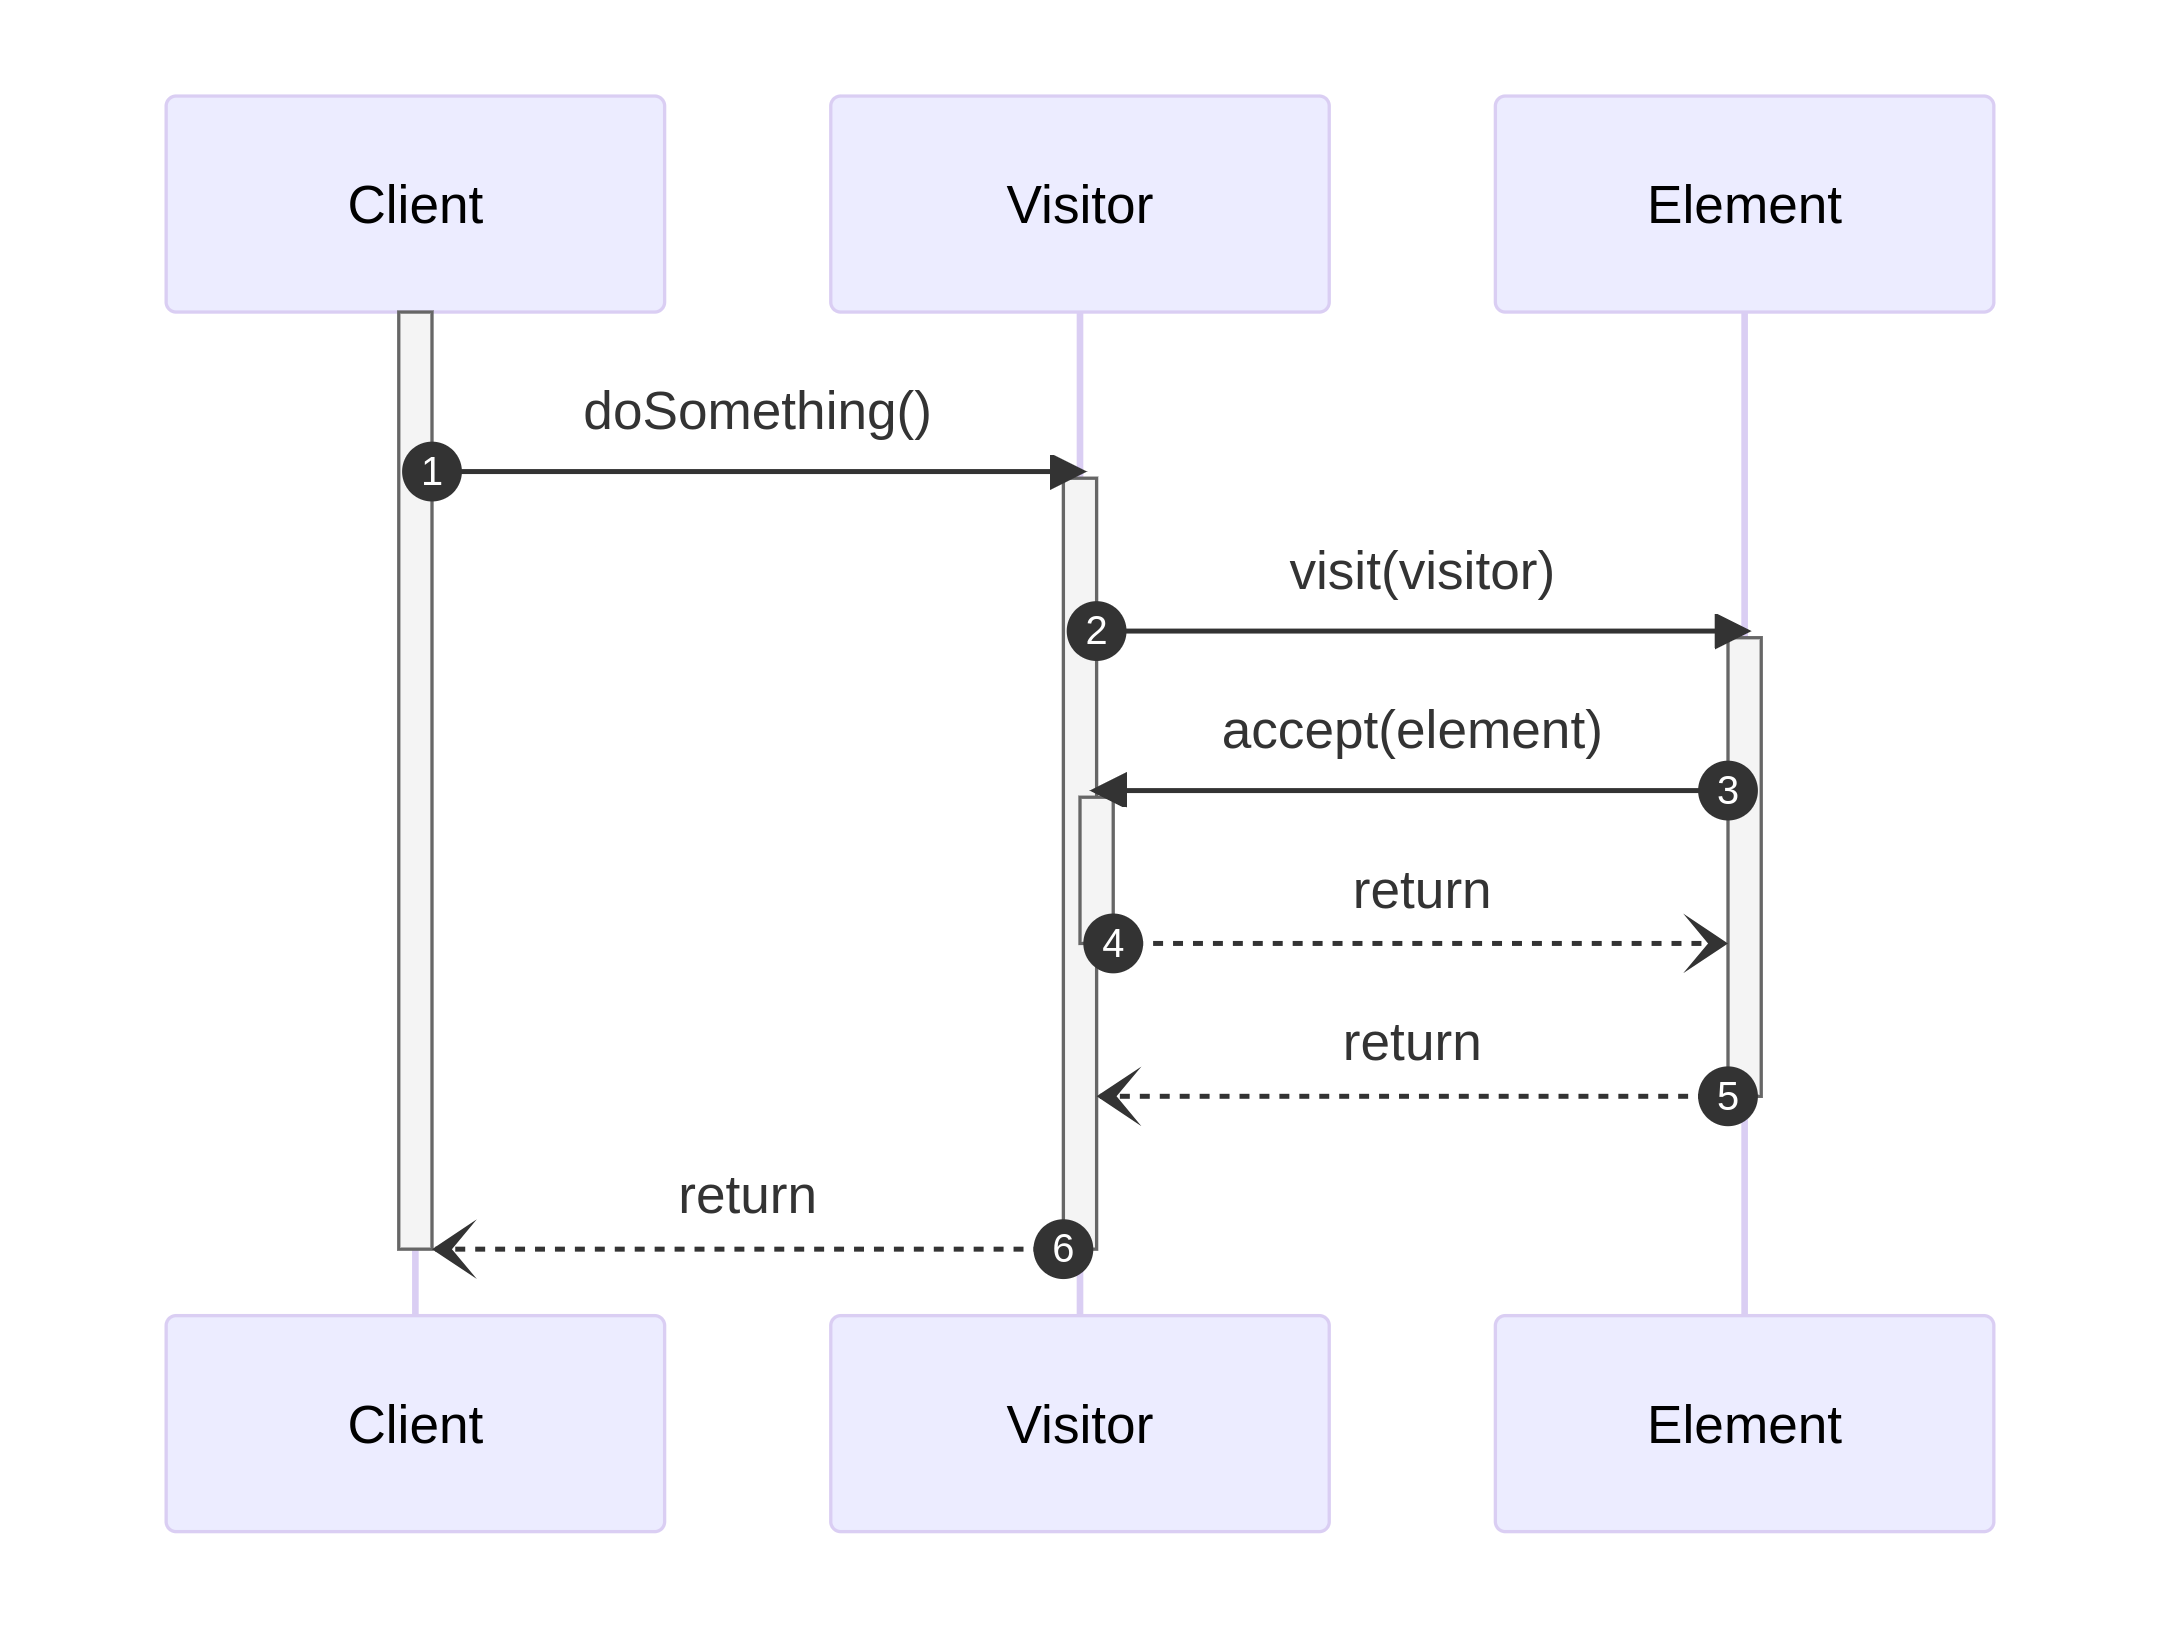
\includegraphics[width=0.75\linewidth]{images/patterns/visitor-seq.png}
	\caption{Sequenzdiagramm des \emph{Visitor-Patterns}. \cite{skobeleva_visitor_2023}}
	\label{fig:visitor-seq}
\end{figure}

\subsubsection*{Konsequenzen}
Durch die Kapselung der Operation in einem \emph{Visitor}, ist es sehr einfach, neue Operationen hinzuzufügen. Es bedarf dazu lediglich eines weiteren \emph{Visitors}. Außerdem kapselt ein\emph{Visitor} die Menge an Operationen auf den Elementen. Zusammengehörige Operationen werden in einer Klasse gesammelt. Nicht zueinander gehörende Operationen befinden sich in unterschiedlichen \emph{Visitors}. Ein weiterer Vorteil eines \emph{Visitors} ist dessen Fähigkeit, während des ''Besuchens'' mehrerer Elemente Informationen über diese zu akkumulieren und im Anschluss gebündelt zu repräsentieren.

Der\emph{Visitor}weist jedoch auch Nachteile auf. Zum einen ist es schwer, weitere konkrete Element-Klassen zu einem System hinzuzufügen, welches bereits eine Reihe an \emph{Visitors} besitzt. Da ein\emph{Visitor} für jeden Typ von Element eine Methode bereitstellen muss, kann ein weiteres Element einen erhöhten Implementierungsaufwand bedeuten. Das \emph{Visitor-Pattern} sollte daher nur verwendet werden, wenn entweder die Menge an Elementklassen abgeschlossen oder die Menge an \emph{Visitor}-Klassen übersichtlich ist. Weiterhin müssen die Elemente dem\emph{Visitor} eine Schnittstelle bereitstellen, welche es dem\emph{Visitor} ermöglicht, seine Operation ausführen zu können. Dies kann dazu führen, dass das Element einen großen Teil seines internen Zustands preisgeben muss, welcher bei nicht-Verwendung dieses Musters gekapselt geblieben wäre. \cite{gamma_design_1995}
\subsection{Factory Method}

\subsubsection*{Problembeschreibung}

Es wird eine Schnittstelle benötigt, um eine Reihe von Objekten erzeugen zu können. Jedes Objekt hat jedoch andere Anforderungen an seine Erzeugung. Eine \emph{Factory-Method} kann eingesetzt werden, wenn eine Klasse kein Wissen darüber besitzt oder besitzen soll, welches konkrete Objekt sie zu erzeugen hat oder wenn eine Klasse die Verantwortlichkeit über diese Entscheidung ihren Subklassen überlassen soll. \cite{gamma_design_1995}

\subsubsection*{Lösung}

Es existiert ein abstrakter Erzeuger (\code{Creator}), welcher eine Schnittstelle bereitstellt, um Produkte (\code{Product}) zu erzeugen. Die Details der Erzeugung dieser Produkte sind in den konkreten Subklassen der Erzeuger-Klasse implementiert. Jeder konkrete Erzeuger kann somit einen Typ von konkretem Produkt (\code{ConcreteProduct}) erschaffen. Das entsprechende Klassendiagramm ist in \autoref{fig:factory-method-class} dargestellt.

\begin{figure}[!ht]
	\centering
	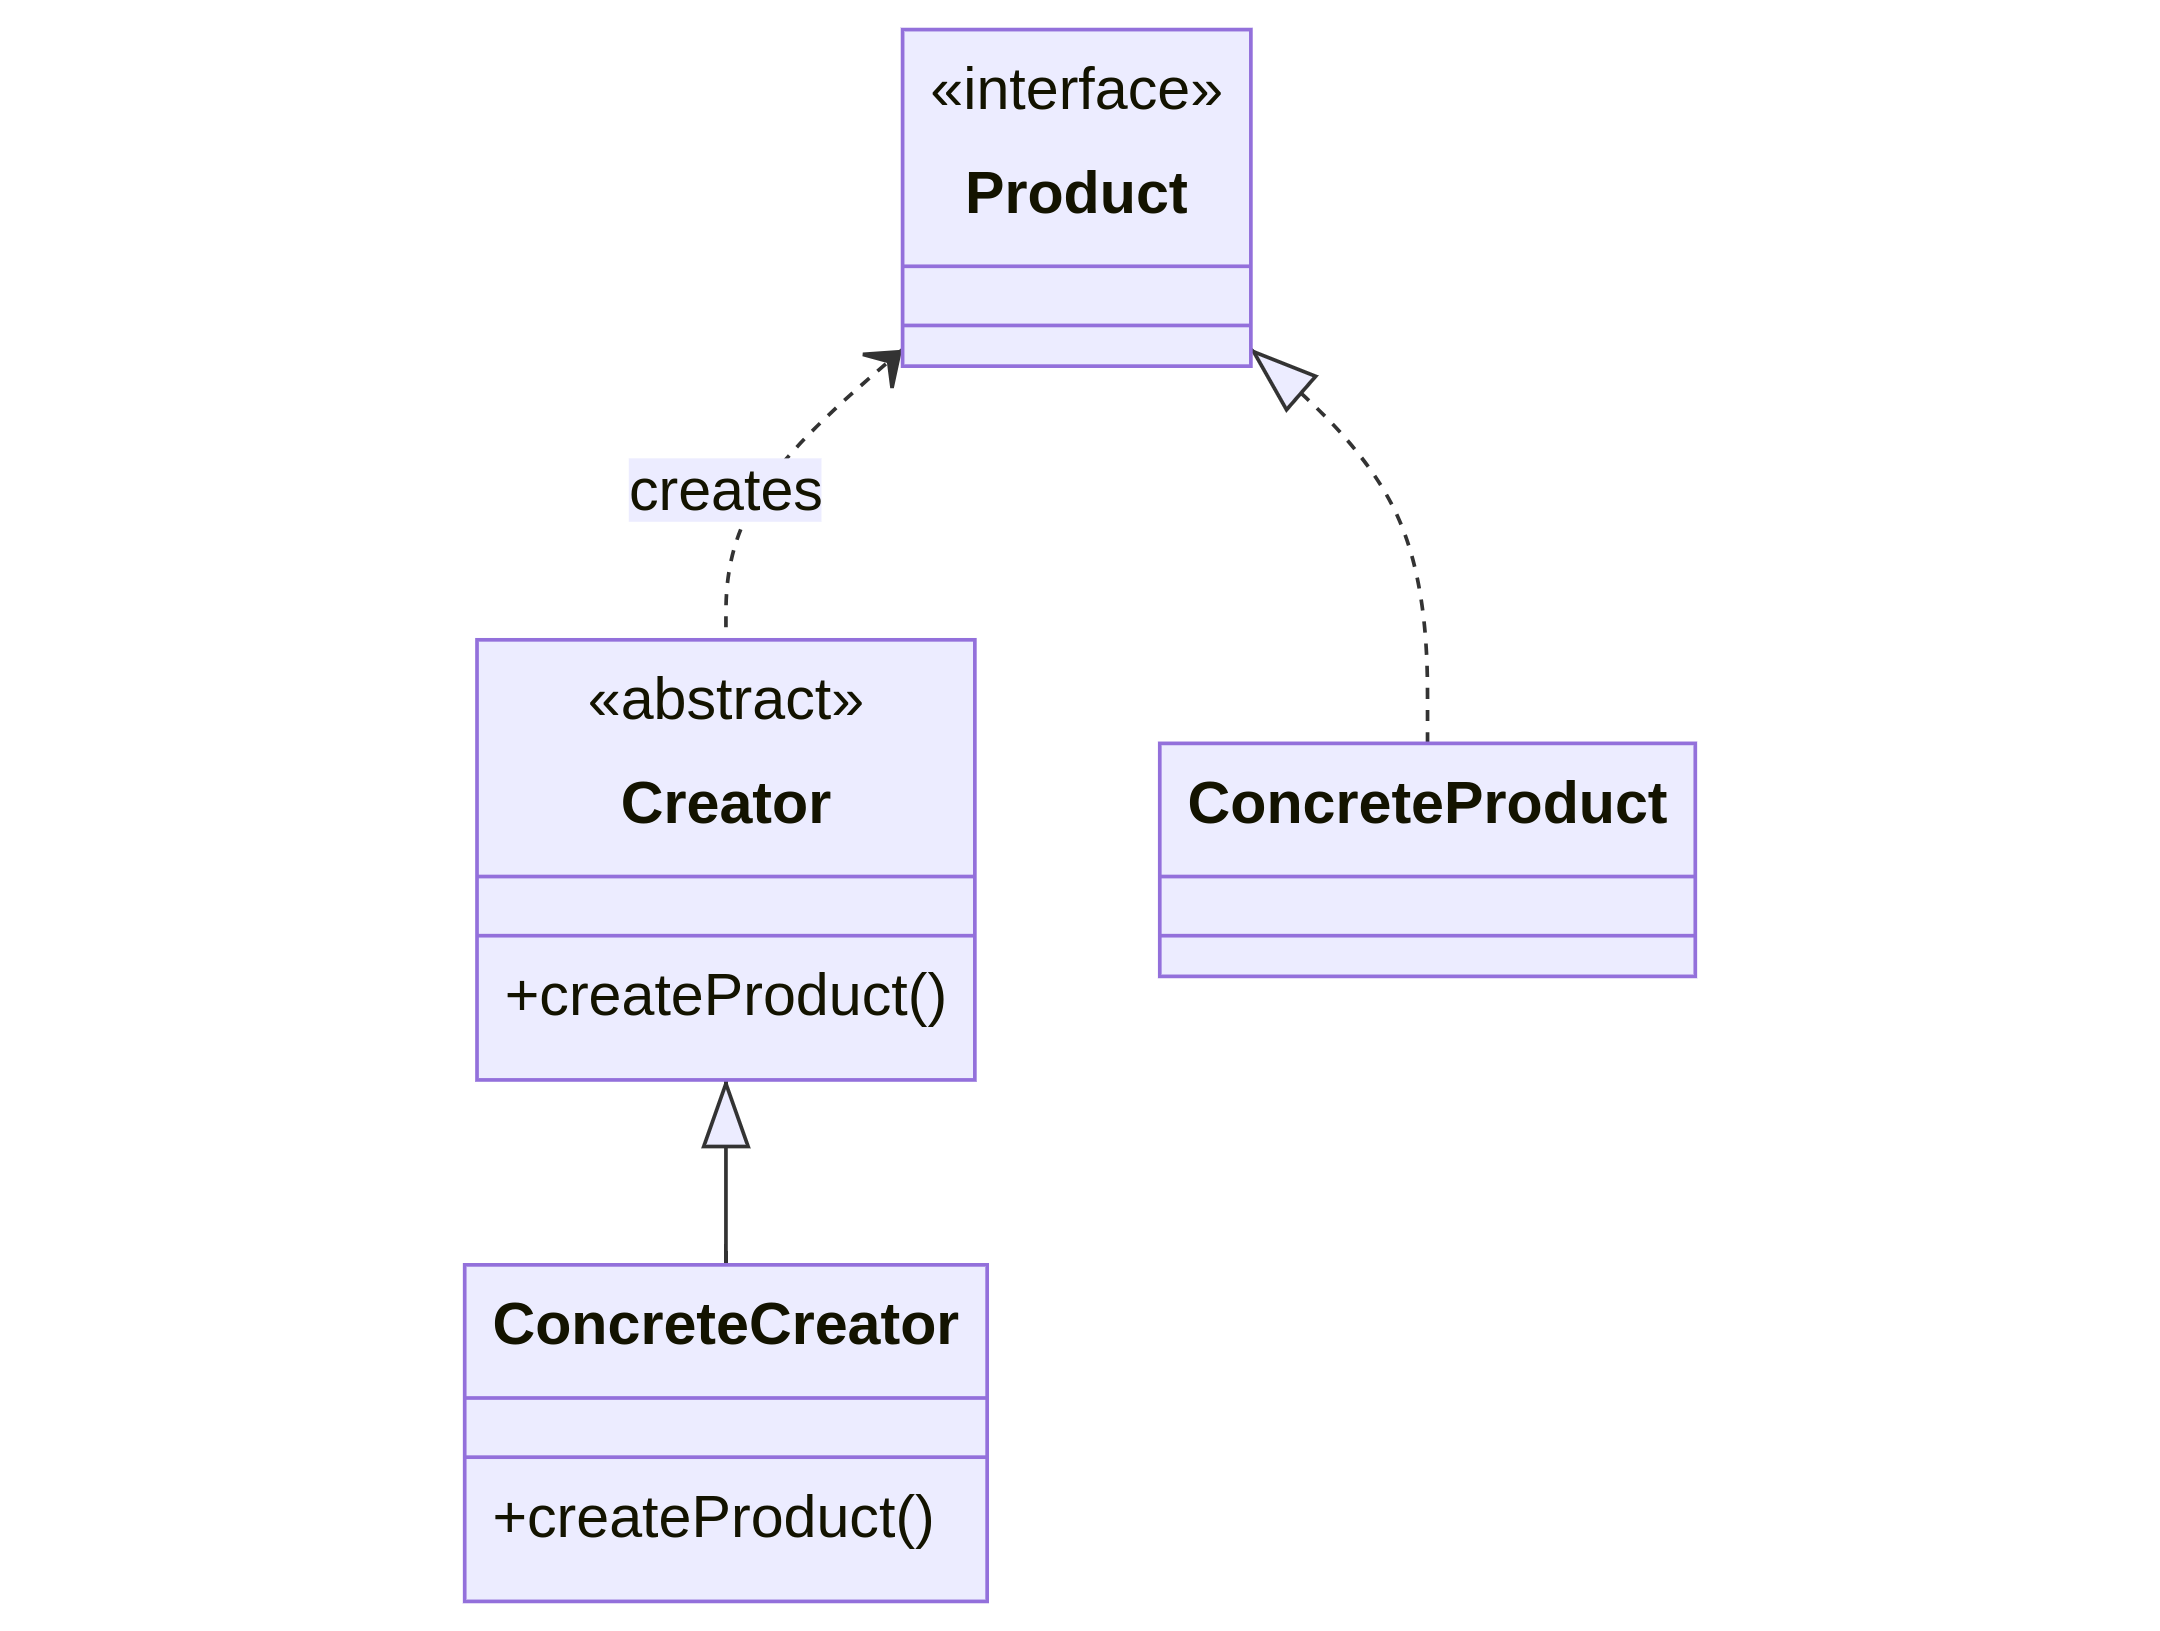
\includegraphics[width=0.75\linewidth]{images/patterns/factory-method-class.png}
	\caption{Klassendiagramm des \emph{Factory-Method}-Musters. Durch die Spiegelung der Vererbungshierarchie von Objekten entstehen Klassen, welche zur Erzeugung der Objekte verwendet werden können. \cite{skobeleva_factory_2023}}
	\label{fig:factory-method-class}
\end{figure}

\subsubsection*{Konsequenzen}
Ein Objekt über eine \emph{Factory-Method} zu erzeugen ist flexibler, als das Objekt direkt über den Konstruktor der Klasse zu instanziieren. Die erzeugende Klasse braucht nur das Interface des abstrakten Erzeugers zu kennen und ist somit in der Lage beliebige konkrete Produkte über deren korrespondierende konkrete Erzeuger zu instanziieren. Hierbei fällt auf, dass die Erzeuger-Klassenhierarchie die Produkt-Klassenhierarchie spiegelt. Für jeden Produkttyp existiert also auch eine Erzeuger-Klasse. Daraus kann sich jedoch auch ein Nachteil ergeben. Zur Nutzung eines Produktes müssen nun stets zwei Subklassen definiert und zur Laufzeit ein weiteres Objekt erstellt werden. Das erhöht die Komplexität. \cite{gamma_design_1995}


	\section{Object-Relational-Mapping}

Für die dauerhafte Speicherung von Daten wird eine Datenbank benötigt. Die Interaktion von objektorientiertem Quelltext mit einer relationalen Datenbank kann den Programmierer vor Herausforungen stellen. Diese und mögliche Lösungen werden in diesem Abschnitt vorgestellt.

\subsection{Objekt-relationale Systeme}
In der Praxis haben sich für die Beschreibung von Datenbanken und Software vor allem zwei verschiedene Paradigmen etabliert. Datenbanken, welche der persistenten Speicherung von Daten dienen, folgen häufig dem relationalen Paradigma. Softwaresysteme hingegen, deren Verhalten und Struktur durch Programmiersprachen beschrieben werden, werden meist objektorientiert modelliert. Da diese beiden Technologien, breite Verwendung finden, ist ihre Kombination innerhalb desselben Systems in der häufig unumgänglich. Solche Systeme nennt man objekt-relationale Systeme. \cite{ireland_understanding_2009}

\subsection{Object-Relational Mapper (ORM)}
Die Aufgabe eines ORM ist es, die Persistenz von Objekten zu gewährleisten \cite{noauthor_what_2023} und dabei gleichzeitig die darunterliegende relationale Datenbank zu abstrahieren. So kann der Programmierer, welcher eine objektorientierte Programmiersprache verwendet, vollständig in einem objektorientierten Kontext arbeiten. Er ist nicht mehr gezwungen, direkt mit der relationalen Datenbank über \emph{SQL} zu kommunizieren. Das ORM stellt dabei eine bidirektionale Abbildung zwischen dem objektorientierten und dem relationalen Modell bereit. Dabei muss sichergestellt werden, dass sowohl die Struktur, als auch die Mechanismen beider Paradigmen korrekt aufeinander abgebildet werden. Die Abbildung der Struktur beschäftigt sich mit der Zuordnung von Tabellen zu Klassen. Die Abbildung der Mechanismen behandelt unter anderem die Navigation durch Objektreferenzen und das Schreiben und Lesen von Daten. \cite{ireland_understanding_2009}

\subsection{Hindernisse}
Die Unterschiede zwischen beiden Paradigmen rufen eine Reihe von Problemen hervor, welche das ORM lösen muss. Diese Probleme sind nach \cite{ireland_understanding_2009} die folgenden:
\begin{itemize}
    \item Es muss eine Abbildung zwischen den Strukturen beider Paradigmen gefunden werden. Eine relationale Datenbank unterstützt weder Klassenhierarchien noch Spalten, die mehrere Elemente beinhalten können.
    \item Zeilen innerhalb einer Relation haben eine festgeschriebene Struktur. Objekte hingegen können eine dynamische Struktur besitzen. Die Frage ist, wie sich die Objektstruktur in der Datenbank abbilden lässt.
    \item Während der Zustand eines Objektes durch Kapselung geschützt ist, sind alle Daten einer relationalen Datenbank öffentlich. Das Problem besteht in der Abbildung dieser Kapselung.
    \item \enquote{Identität} hat innerhalb der beiden Paradigmen unterschiedliche Bedeutungen. Objekte gelten als identisch, wenn sie die gleiche Speicheradresse besitzen. Identische Zeilen hingegen zeichnen sich durch einen gleichen Primärschlüssel aus. Das kann zu Problemen führen, wenn zwei nicht-identische Objekte mit gleichem Primärschlüssel erzeugt werden.
    \item Referenzen in objektorientierten und relationalen Modellen besitzen unterschiedliche Richtungen. Entsprechend muss die Navigation durch die Modelle abgebildet werden.
    \item In der Praxis kann es vorkommen, dass die Datenbank und die darauf aufbauende Software von unterschiedlichen Teams gepflegt werden. Außerdem besteht die Möglichkeit, dass eine Datenbank von mehreren Softwaresystemen genutzt wird. Dabei gilt es, eine einheitliche Kommunikation zu gewährleisten.
\end{itemize}
Jedes ORM konzentriert sich auf die Aspekte der zu leistenden Abbildung unterschiedlich stark. So kann der Fokus beispielsweise mehr auf der strukturellen Abbildung zwischen Klassen und Tabellen liegen oder auf der korrekten Abbildung der Mechanismen. Es gibt daher keine einheitliche oder richtige Lösung. Entsprechend ist die Trennung zwischen objektorientiertem und relationalem Paradigma nie vollständig und hängt vom Einzelfall und den Bedürfnissen des Anwenders ab.

\subsection{peewee}
Für unser Softwareprojekt haben wir das ORM \emph{peewee}\footnote{\url{https://github.com/coleifer/peewee}} \cite{leifer_coleiferpeewee_2023} ausgewählt. Da das ORM einer der Grundsteine unseres Projektes darstellt, stand die Auswahl des ORM am Anfang Planungsprozesses. Daher war es uns nicht möglich, das ORM  anhand der Anforderungen unserer Softwarearchitektur auszuwählen. Diese stand zu diesem Zeitpunkt, aufgrund der agilen Arbeitsweise unseres Teams, noch nicht in ausreichendem Detailgrad zur Verfügung. Wir haben die Entscheidung stattdessen anhand der allgemeinen Funktionsübersicht und der Benutzerfreundlichkeit getroffen. Zur Auswahl stand alternativ das ORM \emph{SQLAlchemy} \cite{noauthor_sqlalchemy_2023}. Obwohl \emph{SQLAlchemy} einen größeren Funktionsumfang bietet, ist \emph{peewee} einfacher zu bedienen und man erreicht viele der meistbenutzten Funktionen mit weniger Code. Da dies zugunsten der Entwicklungsgeschwindigkeit geht, haben wir uns letztendlich für \emph{peewee} entschieden. Außerdem sinkt die Wahrscheinlichkeit für das Begehen von Fehlern mit weniger Code.

Im Folgenden wird eine Reihe von Grundfunktionalitäten von \emph{peewee} vorgestellt, welche in unserem Projekt häufig Verwendung fanden und die auch im Rahmen dieser Arbeit eine Rolle spielen.

\subsubsection*{Definition von Modellen}

Als ein Modell wird im Kontext von \emph{peewee} eine Klasse bezeichnet, deren Objekte sich in der verknüpften Datenbank ablegen lassen. Wie in \autoref{code:peewee-model} zu erkennen ist, lassen sich Modelle definieren, indem die betroffene Klasse von \code{peewee.Model} erbt. Die Verknüpfung zur Datenbank lässt sich durch die Definition des Feldes \code{db} in der Klasse \code{Meta} herstellen. Diese Verknüpfung muss innerhalb einer Klassenhierarchie nur einmal in der obersten Superklasse definiert werden.

\lstset{language=python}
\begin{lstlisting}[caption={Python-Code zur Definition eines \emph{peewee}-Modells. Es modelliert eine Person mit einem Namen und einem Geburtstag. Weiterhin besitzt die Klasse das nicht-persistente Feld \code{age}. \cite{noauthor_quickstart_2023}}, label=code:peewee-model]
class Person(Model):
    class Meta:
        db = SqliteDatabase('people.db')

    name = CharField()
    birthday = DateField()
    age: int
\end{lstlisting}

Der Klasse können dann beliebige Attribute und auch Methoden zugewiesen werden. Soll ein Attribut persistent sein, soll es also in der Datenbank abgelegt werden, so muss ihm in der Klassendefinition ein Feld vom Typ \code{peewee.Field} zugewiesen werden. Über den Subtyp dieses Feldes wird der Typ der korrespondierenden Spalte in der Datenbanktabelle festgelegt. Andere Attribute, wie \code{age} in \autoref{code:peewee-model} sind Teil des Objektes, aber nicht persistent.

\subsubsection*{Speichern von Objekten}

Objekte lassen sich auf mittels zwei verschiedener Methoden in der Datenbank ablegen. Jede Modell-Klasse erbt die Methode \code{create} von \code{peewee.Model}. Diese nimmt die gleichen Argumente entgegen wie der eigentlich Konstruktor der Klasse. Wird \code{create} aufgerufen, so wird eine Instanz der Klasse erstellt, in die Datenbank geschrieben und im Anschluss zurückgegeben, wie in \autoref{code:peewee-storing1} ersichtlich wird.

\lstset{language=python}
\begin{lstlisting}[caption={Python-Code zum Erzeugen eines Personen-Objektes und zur Speicherung in der Datenbank in einem Schritt.  \cite{noauthor_quickstart_2023}}, label=code:peewee-storing1]
    uncle_bob = Person.create(name='Bob', birthday=date(1960, 1, 15))
\end{lstlisting}

Alternativ dazu kann das Objekt auch direkt über den Konstruktor erzeugt werden, wie in \autoref{code:peewee-storing2} zu erkennen. Durch anschließenden Aufruf von \code{save} wird das Objekt dann in die Datenbank gelegt. Diese Methode bietet den Vorteil, dass das Objekt nicht zwangsläufig gespeichert werden muss. Auch erfüllt \code{save} die Funktion der Aktualisierung eines Objektes in der Datenbank, nachdem ein bereits existierendes Objekt verändert wurde.

\lstset{language=python}
\begin{lstlisting}[caption={Python-Code zum Erzeugen eines Personen-Objektes und zur anschließenden Speicherung in der Datenbank.  \cite{noauthor_quickstart_2023}}, label=code:peewee-storing2]
    uncle_bob = Person(name='Bob', birthday=date(1960, 1, 15))
    uncle_bob.save()
\end{lstlisting}

\subsubsection*{Datenabfragen}

Das Abfragen von Daten orientiert sich in \emph{peewee} an den Konzepten von SQL, bildet die \emph{SQL}-Schlüsselwörter jedoch auch Methoden ab. \autoref{code:peewee-query} zeigt eine einfache Datenabfrage die zu dem \emph{SQL}-Statement in \autoref{code:sql-query} äquivalent ist.

\lstset{language=python}
\begin{lstlisting}[caption={Python-Code zum Abfragen eines Objektes aus der Datenbank.  \cite{noauthor_quickstart_2023}}, label=code:peewee-query]
    grandma = Person.select().where(Person.name == 'Grandma .L').get()
\end{lstlisting}

\lstset{language=sql}
\begin{lstlisting}[caption={\emph{SQL}-Abfrage mit SELECT und WHERE.}, label=code:sql-query]
    SELECT * FROM Person WHERE name = 'Grandma L.';
\end{lstlisting}

	\section{Die Smard-API}

Die Smard-API\cite{noauthor_bundesapismard-api_nodate} ist eine von der Bundesnetzagentur bereitgestellte Schnittstelle zum Abrufen von Stromproduktionsdaten in Deutschland. Sie liefert die Menge produzierten Stromes in Abhängigkeit von der Zeit. Die Daten werden in verschiedenen zeitlichen Auflösungen, Jahresdaten bis hin zu 15 Minuten-Intervallen, bereitgestellt. Räumlich lassen sich die Daten bis auf eine Regelzone\footnote{''Als Regelzone wird ein räumlich abgegrenztes Netzgebiet bezeichnet für das ein Übertragungsnetzbetreiber verantwortlich ist.''\cite{noauthor_smard_nodate}} eingrenzen. Weiterhin lassen sich die Daten nach dem Energieträger filtern. So besteht die Möglichkeit, Daten speziell für Braunkohle zu erhalten.\\
\\
Bei der Smard API handelt es sich um eine statische API. Das bedeutet, die Antwort auf eine Anfrage wird nicht für jeden Benutzer zusammengestellt. Stattdessen existiert eine Menge von JSON-Dateien, von denen je nach Anfrage eine ausgeliefert wird. Die API stellt zwei Arten von Dateien zur Verfügung. Für jede Kombination aus zeitlicher und räumlicher Auflösung und Filter gibt es eine Index-Datei. Diese beinhaltet eine Liste von Zeitstempeln. Jeder Zeitstempel ist mit einer Daten-Datei assoziiert. Durch Verwendung des Zeitstempels kann die zugehörige Daten-Datei heruntergeladen werden. Diese enthält eine Liste von Paaren aus Zeitpunkt und produzierter Energiemenge in MWh. Die Paare sind aufsteigend nach Zeitpunkten sortiert und der erste Zeitpunkt entspricht dem verwendeten Zeitstempel.

	\chapter{Hauptteil}
	\section{Die Berechnung des Kohlebedarfs}
\todo{Deadline: 24.06.}
\todo{Hier gehe ich detailliert darauf ein, wie aus historischen Stromverbrauchsdaten der Bundesnetzagentur den Kohlebedarf der Kraftwerke für eine bestimmte Zeitperiode berechne. Im Anschluss erkläre ich, wie ich aus dem Kohlebedarf die Anzahl der zu erzeugenden Züge ermittle und wie ich entscheide, wann diese innerhalb der Simulation erzeugt werden sollen. Ich gehe auf die von mir getroffenen Annahmen ein und leite Schritt für Schritt durch die Berechnung. Ich erkläre auch, an welchen Stellen es weshalb zu Ungenauigkeiten kommen kann. Soweit es mir möglich ist, werde ich die Ergebnisse anhand echter Daten validieren.}
	\section{Architekturdiskussion}
\todo{Deadline: 28.06.}
\todo{Hier diskutiere ich die Architektur der einzelnen Teile, für die ich verantwortlich war. Ich zeige Klassen- und Sequenzdiagramme und lege dar, weshalb bestimmte Design-Entscheidungen getroffen (oder nicht getroffen) wurden.}
\subsection{Die Datenbank}

Das in unserem System verwendete Datenbank-Management-System ist \emph{Postgres}. Es läuft in einem eigenen \emph{Docker}-Container. Als Datenbankschnittstelle verwendeten wir das ORM \emph{peewee}, welches Tabellen einer relationalen Datenbank auf sogenannte Modell-Klassen abbildet. Da jede unserer Modell-Klassen weitere Funktionalität benötigt, haben wir eine abstrakte Modell-Klasse (\code{BaseModel}) definiert, welche als Superklasse für jede weitere Modellklasse dient, und welche selbst von \code{peewee.Model} erbt, wie in \autoref{fig:database-class} zu erkennen ist. Diese Funktionalitäten sind
\begin{itemize}
	\item die explizite Definition eines Primärschlüssels (\code{id}) mit dem Typ einer Zeichenkette, welcher einen \emph{Universally unique identifier} (UUID) enthält,
	\item Daten, wann ein Objekt erzeugt und wann es zuletzt aktualisiert wurde
	\item und einen menschen-lesbaren Bezeichner (\code{readable\_id}), welcher prozedural erzeugt wird und einer verbesserten Nutzerinteraktion dient.
\end{itemize}
Weiterhin wurde die Methode \code{save} überschrieben aus \code{peewee.Model} überschrieben, um darin den Feldern \code{created\_at}, \code{updated\_at} und \code{readable\_id} ihre Werte zuzuweisen.

\begin{figure}[!ht]
	\centering
	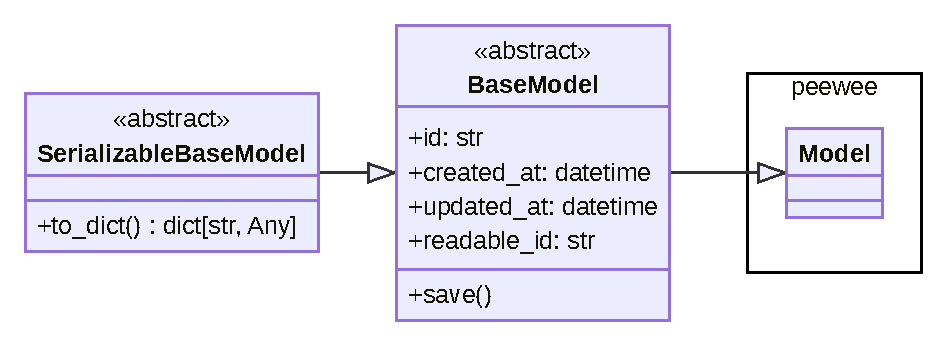
\includegraphics[width=0.75\linewidth]{images/diagrams/database-class.pdf}
	\caption{Klassendiagramm der abstrakten Modell-Klassen des ORM. \code{BaseModel} erbt von \code{peewee.Model}, um weitere Funktionalität hinzuzufügen. Dazu gehören Felder für \code{datetime}-Objekte, welche angeben, wann das Objekt erstellt und aktualisiert wurde. Weiterhin besitzt jedes Objekt eine \code{readable\_id}, welche die Identifizierung durch einen Menschen vereinfachen soll. Davon erbt \code{SerializableBaseModel}, um die Serialisierung von Objekten zu ermöglichen.}
	\label{fig:database-class}
\end{figure}

Von \code{BaseModel} erbt \code{SerializableBaseModel}, welches die zusätzliche Methode \code{to\_dict} implementiert. Damit lässt sich das Objekt JSON-serialisieren, um es bei Bedarf an das Frontend der Anwendung senden zu können.

\begin{figure}[!ht]
	\centering
	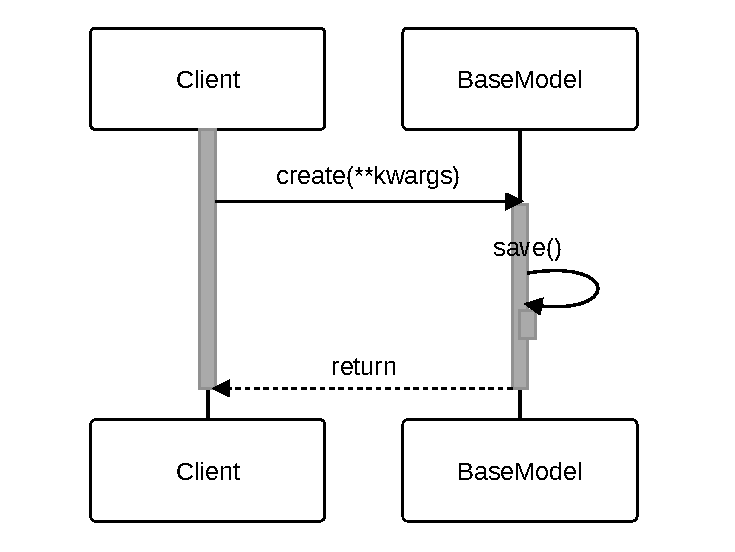
\includegraphics[width=0.75\linewidth]{images/diagrams/database-seq.pdf}
	\caption{Sequenzdiagramm der Erstellung eines Objektes über die Methode \code{create}. In \code{create} wird sowohl das Objekt initialisiert, als auch Selbstaufruf von \code{save} in der Datenbank abgelegt.}
	\label{fig:database-seq}
\end{figure}

Da die hinzugefügten Funktionalitäten in der überschriebenen Methode \code{save} implementiert wurden, sind diese gut in das Modell-System von \emph{peewee} integriert. Da \code{save} auch in \code{create} aufgerufen wird, wie in \autoref{fig:database-seq} zu erkennen, ist die Funktionalität damit automatisch auch bei der direkten Erzeugung eines neuen Objekts gegeben.

Alle im Rahmen unseres Projektes definierten Modell-Klassen erben von \code{BaseModel} oder \code{SerializableBaseModel} und erhalten damit die hinzugefügten Attribute.
\subsection{Der \emph{Spawner}}

Das zentrale Element der Zugerzeugung ist die Klasse \code{Spawner}. Die Architektur aller an der Zeugerzeugung beteiligten Klassen ist in Abbildung \ref{fig:spawner-class} dargestellt. Die Klasse \code{Spawner} erbt, wie die anderen zentralen Klassen des Systems, von der Klasse \code{Component} und erhält damit Zugriff auf den \code{EventBus}, welcher in einem folgenden Abschnitt beschrieben wird, und auf die Methode \code{next\_tick}. Diese Methode wird in jedem Zeitintervall der Simulation einmal aufgerufen und gibt der Komponente die Möglichkeit, auf die Simulation zu reagieren. Weiterhin realisiert die Klasse \code{Spawner} die \code{ISpawnerDisruptor}-Schnittstelle, welche eine Fehlerinjektion\cite{persitzky_fehlerinjektion_2023} ermöglicht. Der \code{Spawner} besitzt die Attribute \code{configuration}, welches im folgenden Abschnitt näher beleuchtet wird, und \code{schedules}, bei dem es sich um eine Liste Abfahrtsplänen (\code{Schedule}-Objekte) handelt.

\begin{figure}[H]
	\centering
	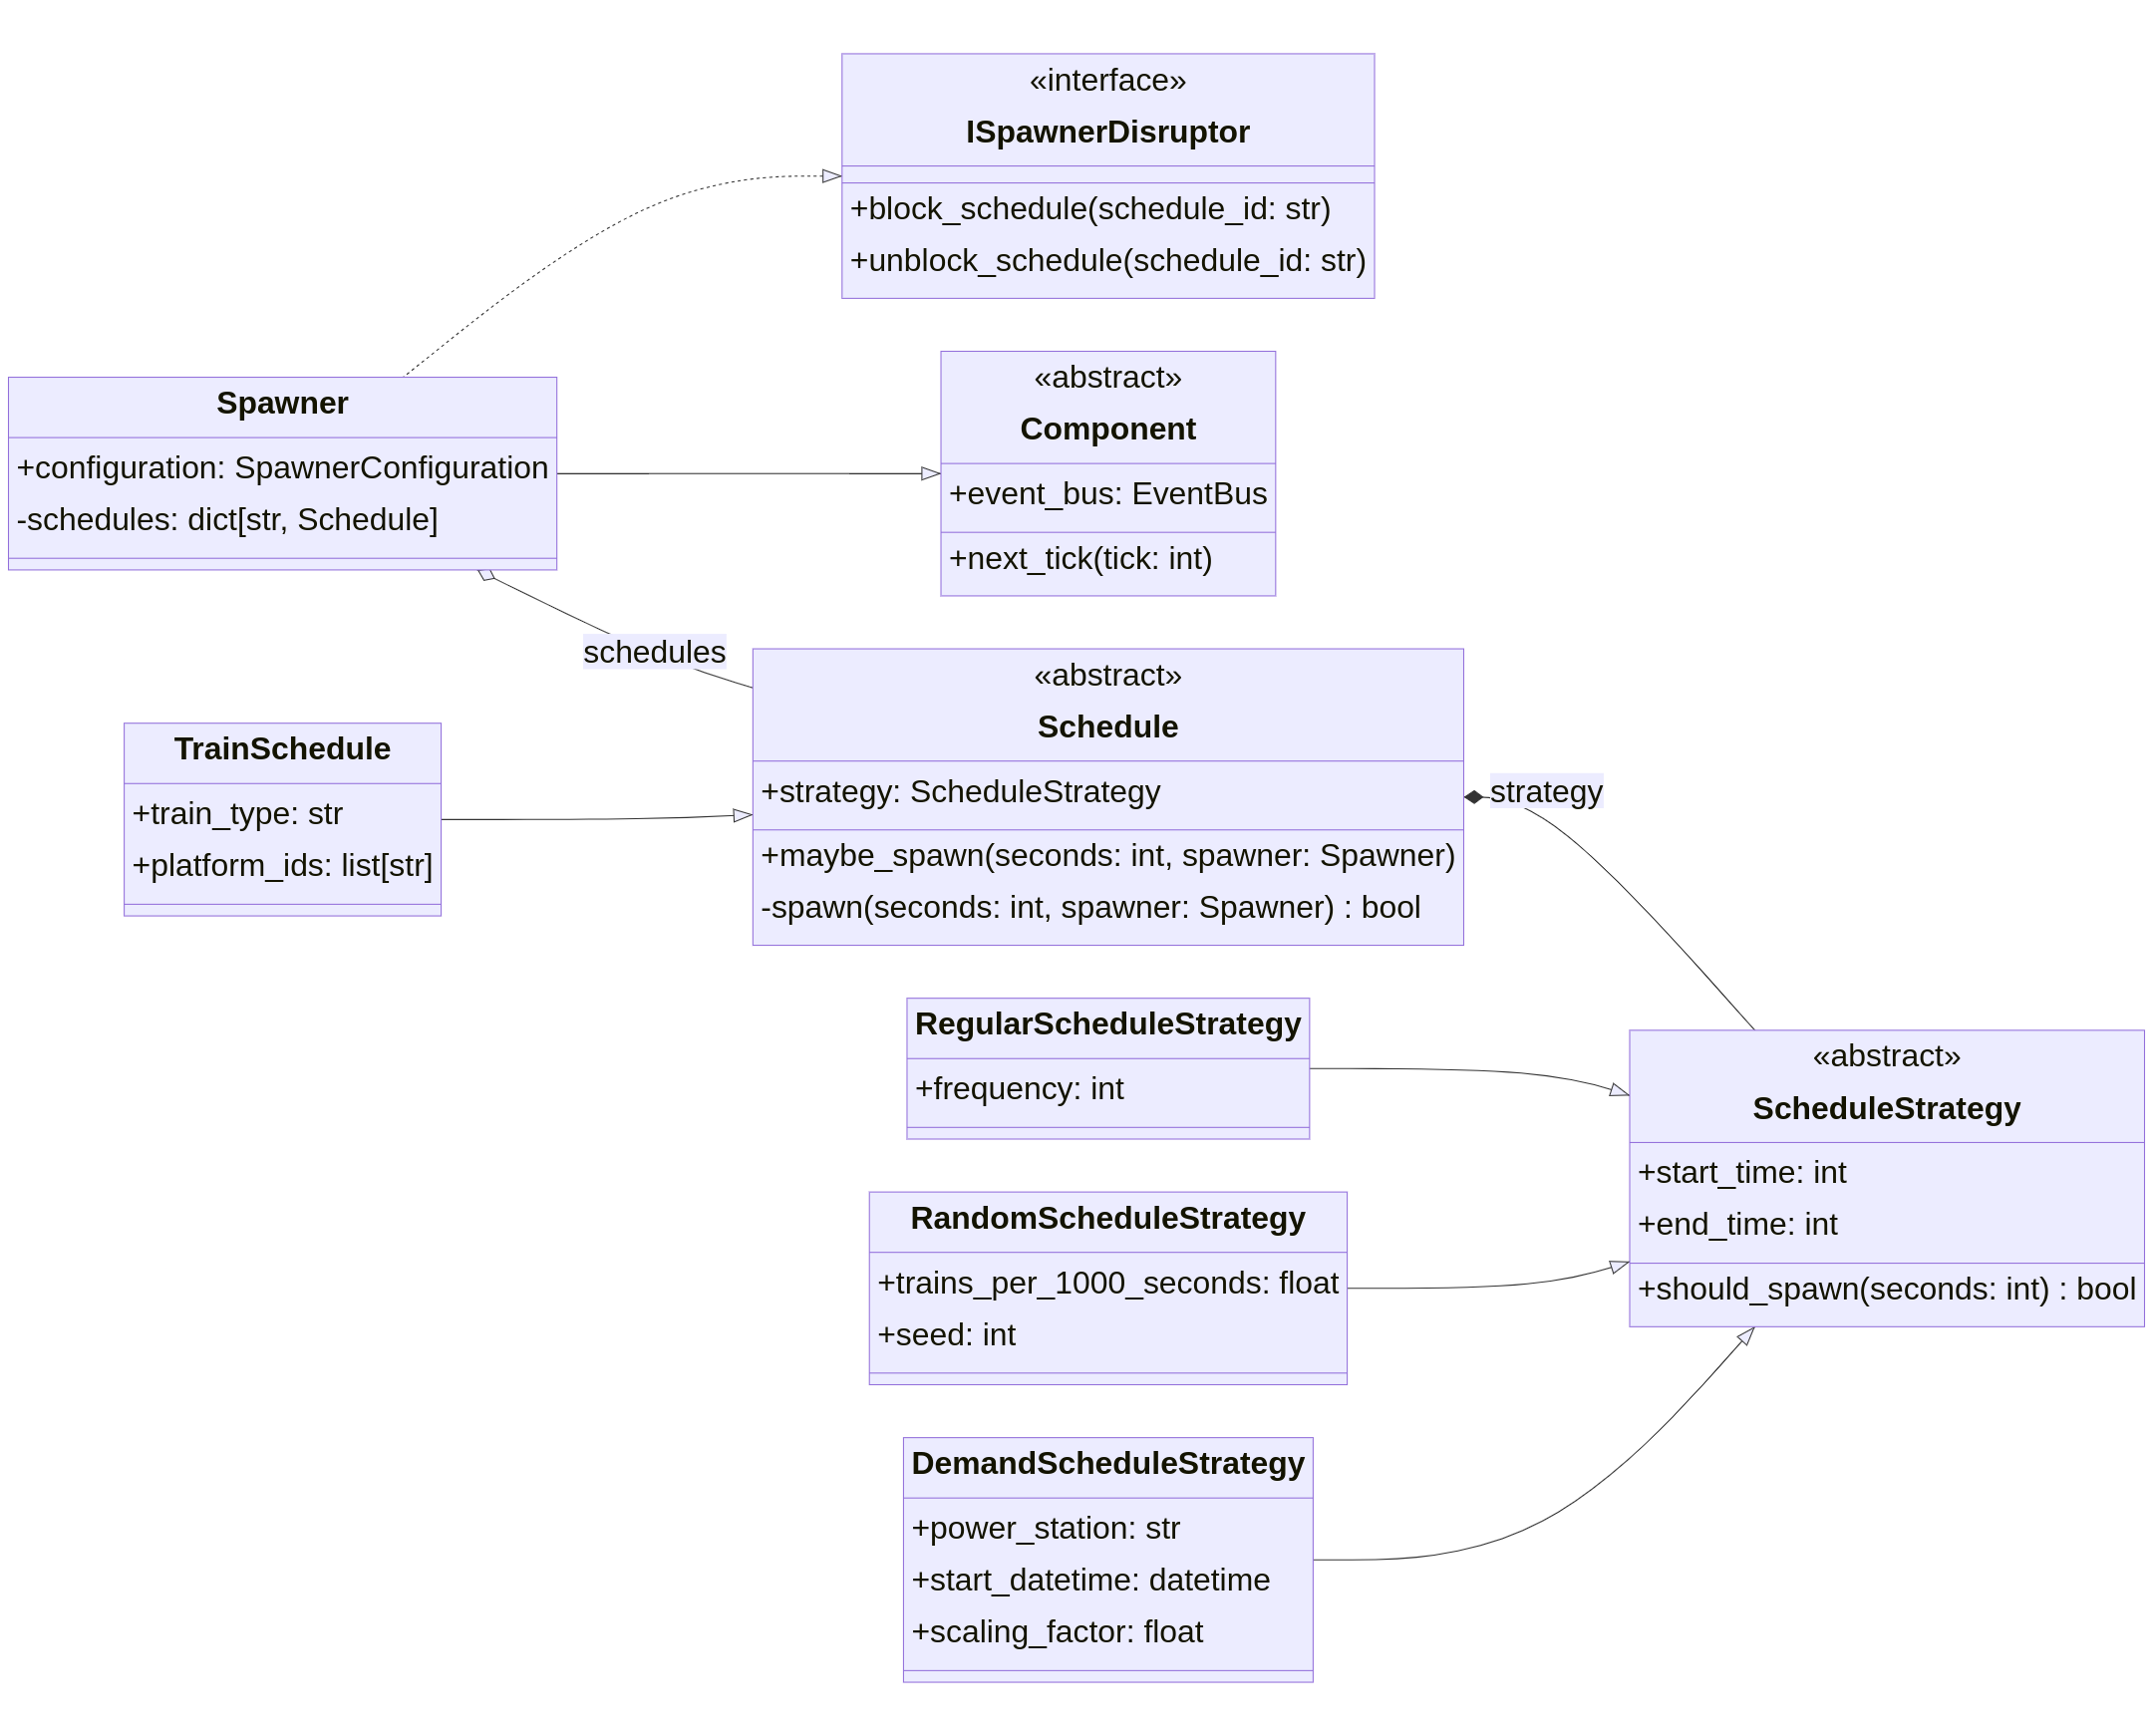
\includegraphics[width=1.0\linewidth]{images/diagrams/spawner-class.png}
	\caption{Klassendiagramm der Zugerzeugung}
	\label{fig:spawner-class}
\end{figure}

Die Klasse \code{Schedule} ist abstrakt und bietet damit die Möglichkeit der Spezialisierung. Die einzige bisher implementierte Spezialisierung ist der \code{TrainSchedule}, welcher speziell für die Erzeugung von Zügen verantwortlich ist. Wir haben uns für eine abstrakte \code{Schedule}-Klasse entschieden, um die Möglichkeit zu haben, das System in Zukunft um Abfahrtspläne anderer Verkehrsteilnehmer zu erweitern. Denkbar wäre bspw. die Simulation von Fußgängern, die gleichzeitig als Passagiere für Personenzüge fungieren. Diese Funktionalität könnte in einer Klasse \code{PedestrianSchedule} implementiert werden, welche ebenfalls von \code{Schedule} erbt. Eine Instanz eines \code{TrainSchedule} Attribute, welche den Zugtyp (\code{train\_type}) und die Liste der anzufahrenden Haltestellen (\code{platform\_ids}) enthalten.\\
\\
Um eine zukünftige Erweiterbarkeit zu gewährleisten, wurde die Klasse \code{Schedule} so implementiert, dass der Algorithmus, welcher die Abfahrzeiten bestimmt, von der eigentlichen \code{Schedule}-Klasse unabhängig ist. Ein \code{Schedule}-Objekt hält eine Referenz auf ein \code{ScheduleStrategy}-Objekt, welches einen Algorithmus zur Bestimmung der Abfahrtszeiten implementiert. Diese Klasse stellt eine Start- und eine Endzeit (\code{start\_time} und \code{end\_time}) bereit, welche die Zeitspanne festlegen, in der die Abfahrtszeiten bestimmt werden. Mit der Methode \code{should\_spawn} kann für eine bestimmte Zeit abgefragt werden, ob ein Zug zu erzeugen ist. Von der abtrakten Klasse \code{ScheduleStrategy} erben die Klassen \code{RegularScheduleStrategy}, \code{RandomScheduleStrategy} und \code{DemandScheduleStrategy}, welche das Verhalten der drei zuvor beschriebenen Abfahrtspläne implementieren.\\
\\
Die Klasse \code{RegularScheduleStrategy} implementiert die regulären Abfahrtspläne und besitzt das Attribut \code{frequency}, welches die Häufigkeit der regelmäßig abfahrenden Züge angibt. Die \code{RandomScheduleStrategy}-Klasse ist für die randomisierten Abfahrtspläne zuständig und besitzt dafür die Attribute \code{trains\_per\_100\_seconds} und \code{seed}, welche die Wahrscheinlichkeit einer Abfahrt und einen Startwert für den Zufallszahlengenerator beinhalten. Letzteres Attribut dient der Reproduzierbarkeit von Simulationsergebnissen. Die \code{DemandScheduleStrategy}-Klasse implementiert die Abfahrtspläne, welche auf dem Kohlebedarf basieren. Die hält die Attribute \code{power\_station} für das betrachtete Kraftwerk, \code{start\_datetime} für das Startdatum der historischen Datenbasis und \code{scaling\_factor}, womit der Kohlebedarf skaliert werden kann, um bspw. eine unvollständige Auslastung eines Kraftwerks zu simulieren.

Abbildung \ref{fig:spawner-seq} zeigt das Verhalten der Zugerzeugung innerhalb eines Zeitintervalls der Simulation. Ein \code{Communicator}-Objekt\footnote{beschrieben in der Arbeit von \citeauthor{kamp_architektur_2023}\cite{kamp_architektur_2023}} sendet \code{nect\_tick} an das \code{Spawner}-Objekt (1). Dieser sendet daraufhin \code{maybe\_spawn} an jedes Element in der Liste \code{schedules} und übergibt sich dabei selbst (2). Durch Aufruf von \code{should\_spawn} wird überprüft, ob ein Zug zu erzeugen ist (3). Ist dies der Fall, ruft das \code{Schedule}-Objekt auf sich selbst \code{spawn} auf (5), was dazu führt, dass \code{spawn\_train} an die übergebene \code{Spawner}-Instanz gesendet wird (6). Dort wird letztendlich die Schnittstelle zu SUMO angesprochen, um einen Zug in die Simulation zu setzen.

\begin{figure}[H]
	\centering
	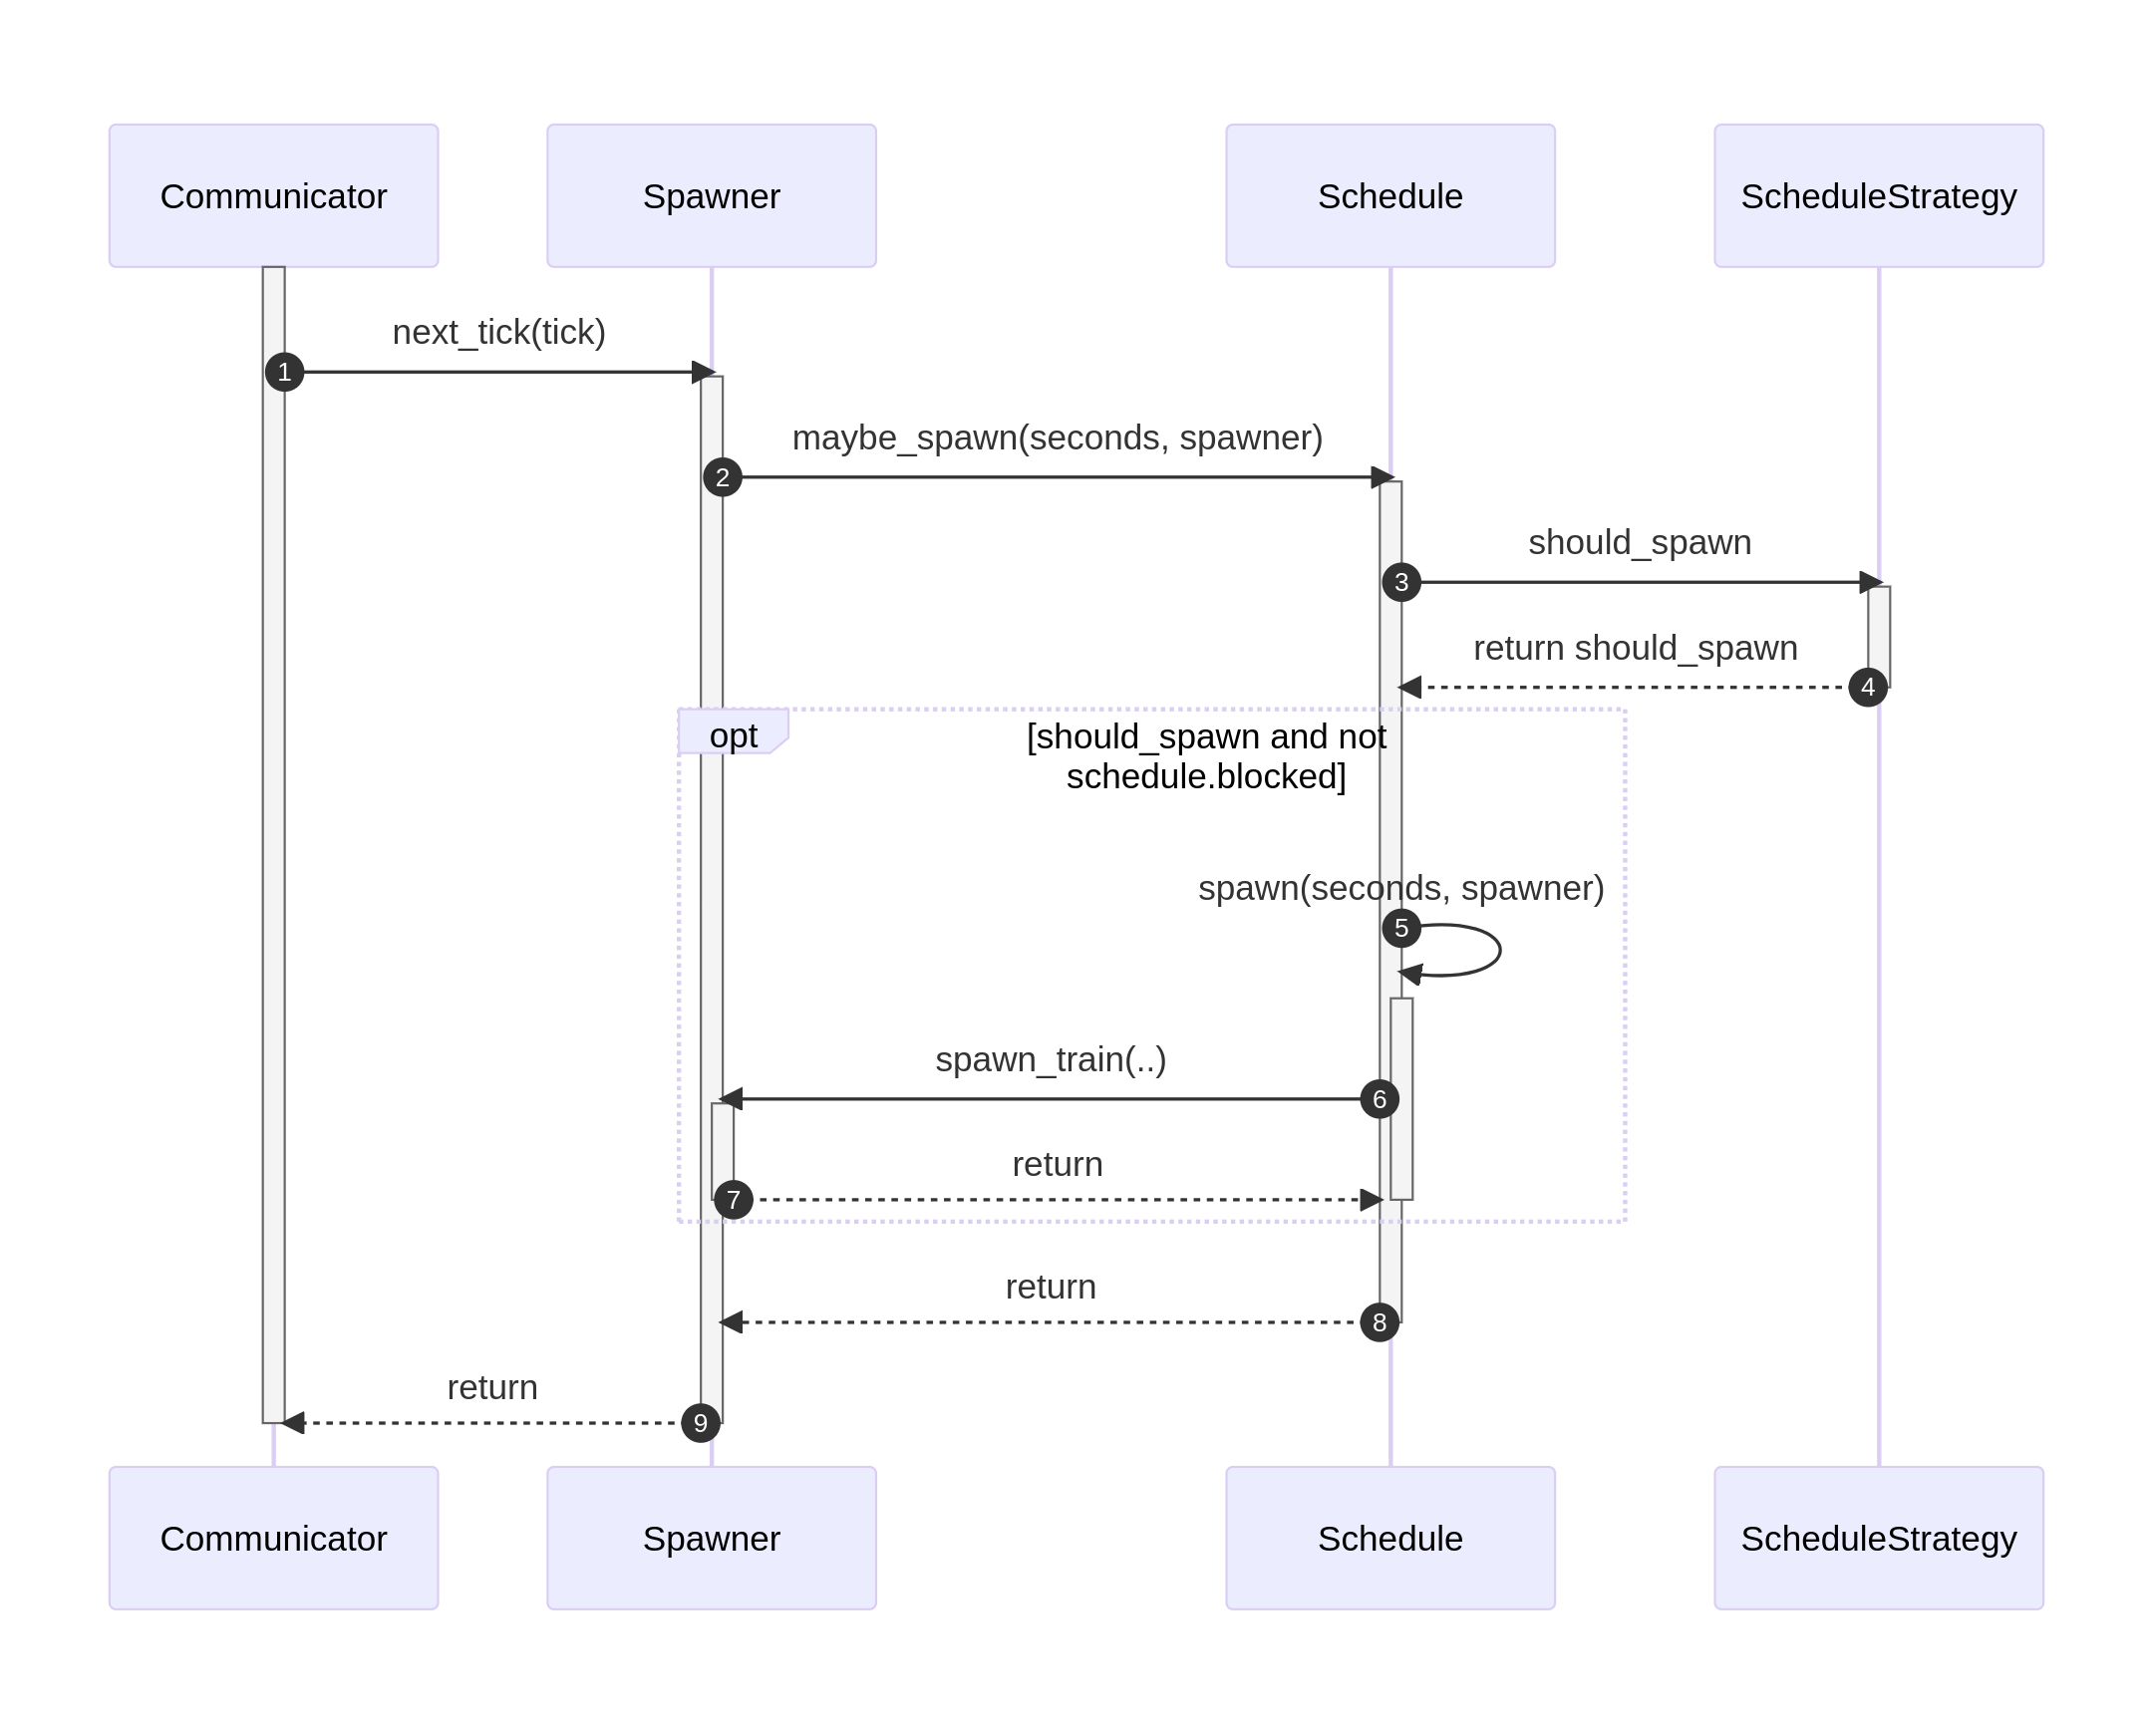
\includegraphics[width=1.0\linewidth]{images/diagrams/spawner-seq.png}
	\caption{Sequenzdiagramm der Zugerzeugung}
	\label{fig:spawner-seq}
\end{figure}

Bei diesem Mechanismus finden zwei Entwurfsmuster Anwendung. Der \code{Spawner} fungiert and \emph{Visitor} und besucht jedes Element in der Liste von \code{Schedule}-Objekten. Über einen \emph{Double-Dispatch} mit den Methoden \code{maybe\_spawn} und \code{spawn\_train} wird dabei erreicht, dass die Verantwortlichkeit der Implementierung zur Erzeugung von Zügen (und zukünftig evtl. weiterer Verkehrsteilnehmer) bei der Klasse \code{Spawner} liegt. Die Entscheidung hingegen wird von den \code{Schedule}-Objekten getroffen. Dadurch lassen sich in Zukunft relativ einfach weitere Arten von \code{Schedule}-Klassen hinzufügen. Die Klasse \code{Spawner} muss dazu nur um jeweils eine weitere Methode erweitert werden. Bei der Methode \code{maybe\_spawn} handelt es sich weiterhin um eine im abstrakten \code{Schedule} implementierte \emph{Template-Method}. Sie gibt den Ablauf der Entscheidung über die Zugerzeugug vor. Die konkreten Implementierungen für \code{spawn} und \code{should\_spawn} liegen jedoch in den konkreten Subklassen von \code{Schedule}  bzw. \code{ScheduleStrategy}. Auch hier ist der Vorteil, dass sich neue Algorithmen zur Bestimmung der Abfahrtszeiten relativ einfach hinzufügen lassen, ohne dass die Klasse \code{Spawner} angepasst werden muss.

\subsection{Die Konfiguration des Spawners}

Die Konfiguration des \emph{Spawners} legt fest, wann und wo in der Simulation Züge erzeugt werden. Eine der Anforderungen an das System ist, dass der Benutzer in der Lage sein muss, diese Konfiguration durchzuführen. Weiterhin ist es wünschenswert, dass die Konfigurationen gespeichert werden können, um die zugehörigen Simulationen erneut oder in abgeänderter Form durchführen zu können. Zu Beginn des Projektes erbten die Klassen \code{Spawner}, \code{Schedule} und \code{ScheduleStrategy} von \code{BaseModel}. Somit ließen sich Instanzen dieser Klassen und ihrer Subklassen direkt in die Datenbank schreiben. Dieser Ansatz wurde jedoch verworfen, da das verwendete ORM \emph{peewee} nicht in der Lage ist, objektorientierte Vererbungshierarchien ausreichend gut abzubilden. \emph{peewee} ordnet jeder Klasse eine Tabelle in der Datenbank zu. Es spielt dabei keine Rolle, ob es sich um eine abstrakte oder eine konkrete Klasse handelt. Ein \code{Schedule}-Objekt kann bspw. ein \code{RegularScheduleStrategy}-Objekt enthalten. Die Klasse \code{Schedule} hat jedoch nur Kenntnis von der abstrakten Klasse \code{ScheduleStrategy}. Die Abbildung durch \emph{peewee} erzeugt daher für die Tabelle \code{Schedule} lediglich einen Fremdschlüssel, der auf die ''abstrakte'' Tabelle \code{ScheduleStrategy} verweist. Referenzen auf abstrakte Klassen lassen sich also mit \emph{peewee} nicht abbilden.\\
\\
Wir haben uns stattdessen für die in \autoref{fig:spawner-config-class} dargestellte Architektur entschieden. Dem \code{Spawner} wird nun ein Konfigurationsobjekt (\code{SpawnerConfiguration}) zugewiesen. Über eine $m$:$n$-Beziehung, die durch die Klasse \code{SpawnerConfiguratioXSchedule} bereitgestellt wird, können einem \code{SpawnerConfiguration}-Objekt mehrere \code{ScheduleConfiguration}-Objekte zugewiesen werden, welches alle Informationen für ein \code{Schedule}-Objekt und ein dazugehöriges konkretes \code{ScheduleStrategy}-Objekt beinhaltet. Die Liste der anzufahrenden Haltestellen wird über die Klasse \code{ScheduleConfigurationXSimulationPlatform} referenziert. Über das Attribut \code{index} kann die Reihenfolge der Haltestellen abgebildet werden. Bei diesem Vorgehen ist zu beachten, dass die $m$:$n$-Beziehungen aus der Datenbank nicht vor dem Programmierer versteckt wurden. Stattdessen wurden sie 1:1 in das objektorientierte Paradigma übernommen. Weiterhin gibt es keine Subklassen von \code{Schedule} und \code{ScheduleStrategy} mehr. Sämtliche Attribute der Subklassen finden sich in \code{ScheduleConfiguration} wieder. Entsprechend wird stets nur eine Teilmenge dieser Attribute verwendet. Um die Subklassen dennoch abzubilden, existieren die Felder \code{schedule\_type} und \code{strategy\_type}. Das hier beschriebene Problem wurde bei der Auswahl des ORM nicht vorhergesehen. Um allerdings nicht ein neues ORM in das System integrieren zu müssen, haben wir uns für diese Lösung entschieden. Sie bot einen Zeitvorteil und funktionierte ausreichend gut.

\begin{figure}[!ht]
	\centering
	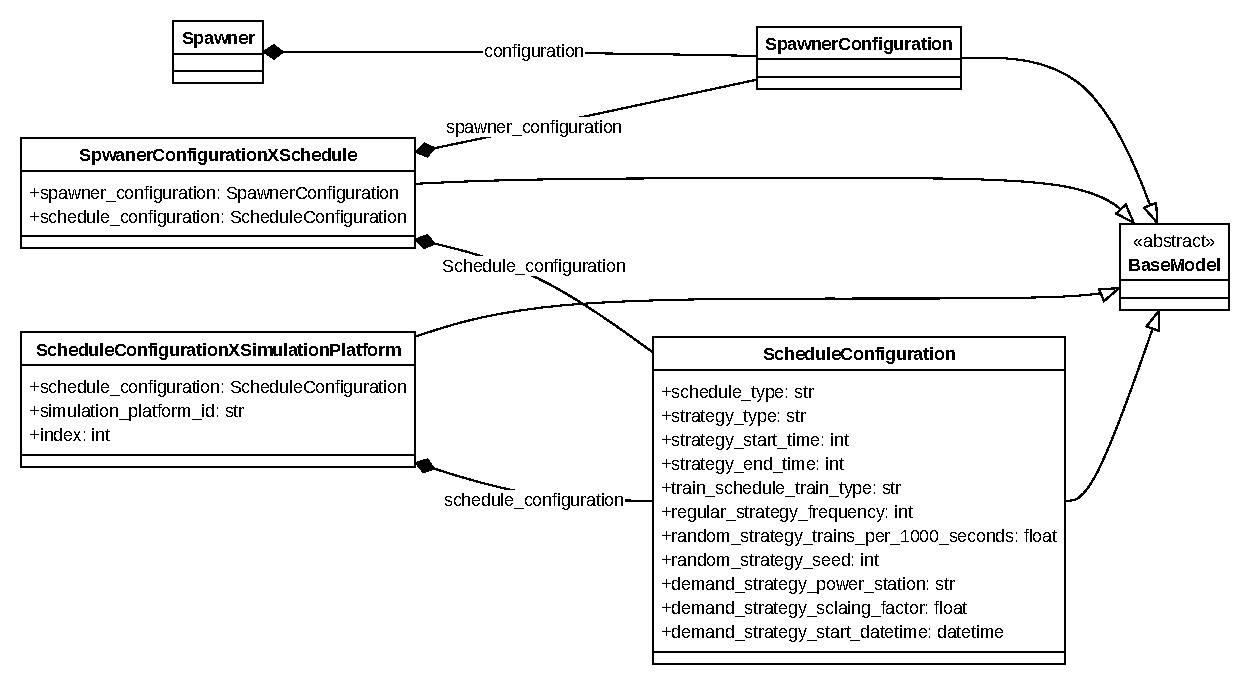
\includegraphics[width=1.0\linewidth]{images/diagrams/spawner-config-class.pdf}
	\caption{Klassendiagramm der \emph{Spawner}-Konfiguration. Die Klasse \code{Spawner} besitzt eine Referenz auf ein \code{SpawnerConfiguration}-Objekt. Dieses ermöglicht über \code{SpawnerConfiguratioXSchedule}-Objekte die Referenzierung von \code{ScheduleConfiguration}-Objekten, welche die Informationen für die Abfahrtspläne enthalten. Die Haltestellen werden über \code{ScheduleConfigurationXSimulationPlatform}-Objekte referenziert. Alle Klassen, bis auf \code{Spawner} erben von \code{BaseModel} und sind damit in der Datenbank abgebildet.}
	\label{fig:spawner-config-class}
\end{figure}

Alle zur Konfiguration gehörenden Klassen werden in JSON-serialisierter Form vom Benutzer über die \emph{REST-API} übertragen \cite{kamp_architektur_2023}. Sie werden daraufhin deserialisiert und in der Datenbank abgelegt. Aus diesen Konfigurationsobjekten können dann ein \code{Spawner}, \code{Schedule}-Objekte und \code{ScheduleStrategy}-Objekte erzeugt werden. Dafür wurde das Entwurfsmuster der \emph{Factory-Method} verwendet. \autoref{fig:spawner-factory-class} zeigt, dass die Klassen \code{Schedule} und \code{ScheduleStrategy} bzw. ihre Subklassen ihre eigenen \emph{Factories} sind. Sie besitzen zu diesem Zweck jeweils eine \emph{Klassen}-Methode \code{from\_schedule\_configuration}, welche als \emph{Factory-Method} fungiert.

\begin{figure}[!ht]
	\centering
	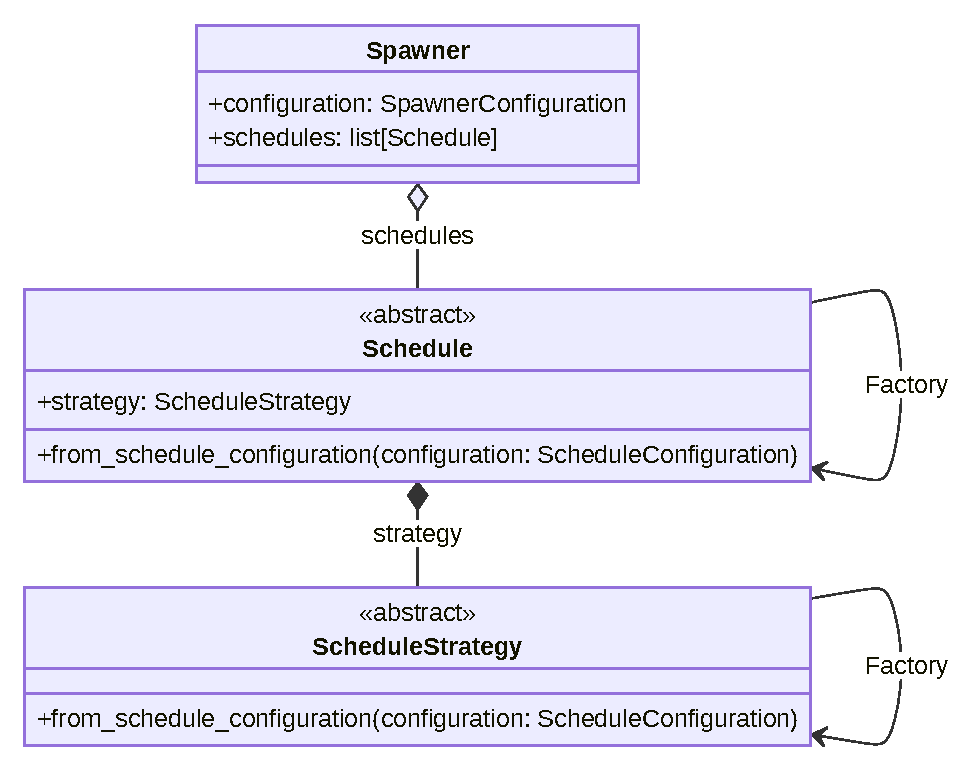
\includegraphics[width=0.80\linewidth]{images/diagrams/spawner-factory-class.pdf}
	\caption{Klassendiagramm der \emph{Spawner}-Konstruktion. Die Klasse \code{Spawner} besitzt eine Liste von \code{Schedule}-Objekten. Die Klasse \code{Schedule} ist ihre eigene \emph{Factory} und kann aus \code{ScheduleConfiguration}-Objekten Instanzen ihrer selbst erstellen. Analog dazu besitzt jedes \code{Schedule}-Objekt eine Referenz auf ein \code{ScheduleStrategy}-Objekt. Auch die Klasse \code{ScheduleStrategy} kann sich selbst mithilfe eines \code{ScheduleConfiguration}-Objektes instanziieren.}
	\label{fig:spawner-factory-class}
\end{figure}

\autoref{fig:spawner-factory-seq} zeigt, wie aus einer Konfiguration, entsprechende Objekte erzeugt werden. Das \code{Spawner}-Objekt ruft für jedes referenzierte \code{ScheduleConfiguration}-Objekt die \emph{Factory-Method} der Klasse \code{Schedule} auf (1). Diese instanziiert daraufhin ein dem Wert des Attributes \code{ScheduleType} entsprechendes \code{Schedule}-Objekt und ein \code{ScheduleStrategy}-Objekt durch Aufruf der \emph{Factory-Method} der Klasse \code{ScheduleStrategy} und erneute Übergabe des Konfigurationsobjektes (2). Beide \emph{Factory-Methods} lesen die benötigten Werte für die Attribute der zu erzeugenden Objekte aus dem Konfigurationsobjekt und geben dann das fertige Objekt zurück. Jedes \code{Schedule}-Objekt kann das erzeugte \code{ScheduleStrategy}-Objekt im Attribut \code{strategy} speichern. Das \code{Spawner}-Objekt kann die erzeugten \code{Schedule}-Objekte in der Liste \code{schedules} speichern.

\begin{figure}[!ht]
	\centering
	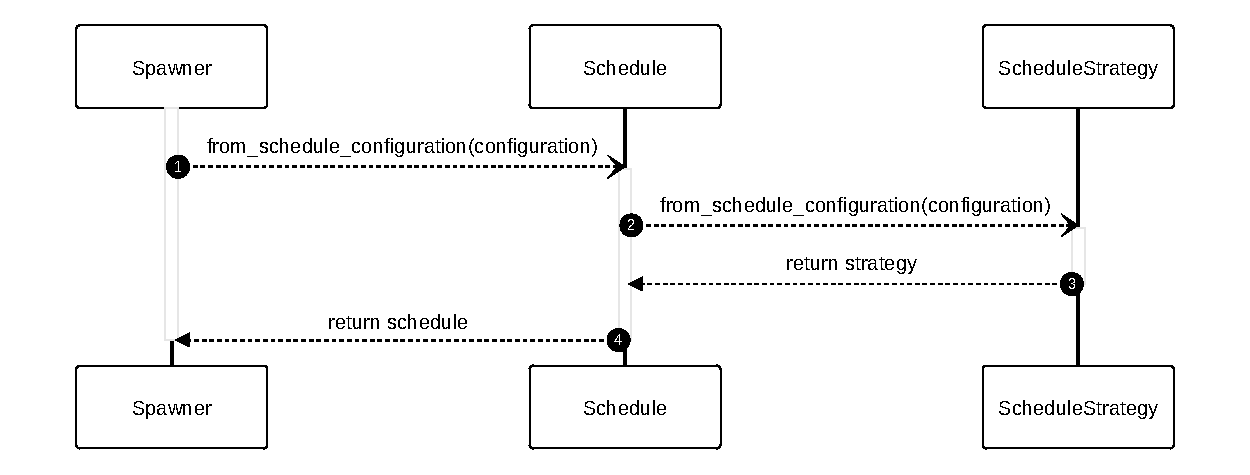
\includegraphics[width=1.0\linewidth]{images/diagrams/spawner-factory-seq.pdf}
	\caption{Sequenzdiagramm der \emph{Spawner}-Konstruktion. Das \code{Spawner}-Objekt ruft für jedes referenzierte \code{ScheduleConfiguration}-Objekt die \emph{Factory-Method} der Klasse \code{Schedule} auf (1). Die Klasse \code{Schedule} tut daraufhin dasselbe für die Klasse \code{ScheduleStrategy} (2). Beide Methoden erzeugen dann eine Instanz ihrer jeweiligen Klassen und geben diese zurück (3, 4).}
	\label{fig:spawner-factory-seq}
\end{figure}

\subsection{Der Eventbus}

Der Eventbus stellt für Softwarekomponenten die Möglichkeit bereit, Ereignisse untereinander auszutauschen. Für jeden Typ von Ereignis stellt er eine $m$:$n$-Beziehung zwischen den Komponenten, welche das Ereignis emittieren und denen, die es empfangen her. Der Eventbus wurde in Zusammenarbeit mit \citeauthor{persitzky_fehlerinjektion_2023} entwickelt. Wir haben uns dazu entschieden, das Entwurfsmuster \emph{Mediator} auf den Eventbus anzuwenden, um zu verhindern, dass die voneinander Abhängigen Komponenten direkt miteinander kommunizieren müssen, was die Kopplung senkt. Weiterhin kapselt der \emph{Mediator} das kommunikationsspezifische Verhalten, was es an einer zentralen Stelle verfügbar macht und den einzelnen Komponenten die Verantwortung abnimmt, Kommunikationsdetails zu kennen.\\
\\
Um eine zu große Komplexität des Eventbus selbst und eine monolithische Struktur zu verhindern, wird als Kommunikationsmechanismus das Entwurfsmuster \emph{Observer} verwendet. Abhängigkeiten zwischen den Komponenten lassen sich so flexibler ändern. Weiterhin ermöglicht dieses Entwurfsmuster, Komponenten auf verschiedenen Abstraktionsniveaus zu verbinden. Wir haben den Nachteil des \emph{Observers} umgangen, dass er stets alle Empfänger benachrichtigt. Dazu wird jeder registrierte Empfänger mit einem Ereignistyp verknüpft. Der Empfänger wird so nur benachrichtigt, wenn ein Ereignis des verknüpften Typs eingangen ist.\\
\\
Um die Kopplung weiter zu verringern, werden beim Eventbus nicht die Empfänger selbst registriert, sondern nur \emph{Callbacks} (Funktionen, welche als Argument übergeben werden, um zu einem späteren Zeitpunkt vom Empfänger des Arguments aufgerufen werden zu können), bei welchen es sich jeweils um Methoden der Empfänger handelt. Dies schränkt die Funktionalität nicht ein, da der Empfännger das Ereginis nachwievor erhält. Der Eventbus muss nun jedoch nur noch Pythons \code{Callable}-Schnittstelle verwenden und benötigt keine Kenntnis mehr über die Kommunizierenden Komponenten. Die Registrierung und die Deregistrierung von Empfängern ist in \autoref{fig:eventbus-register-seq} und \autoref{fig:eventbus-unregister-seq} dargestellt. Für die Registrierung wird das \emph{Callback} und der Ereignistyp (\code{event\_type}) übergeben. Der Eventbus gibt daraufhin ein \emph{Handle} zurück, mit welchem das registrierte \emph{Callback} identifiziert werden kann. Um ein \emph{Callback} zu deregistrieren, lediglich das \emph{Handle} and den Eventbus übergeben werden.

\begin{figure}[!ht]
	\centering
	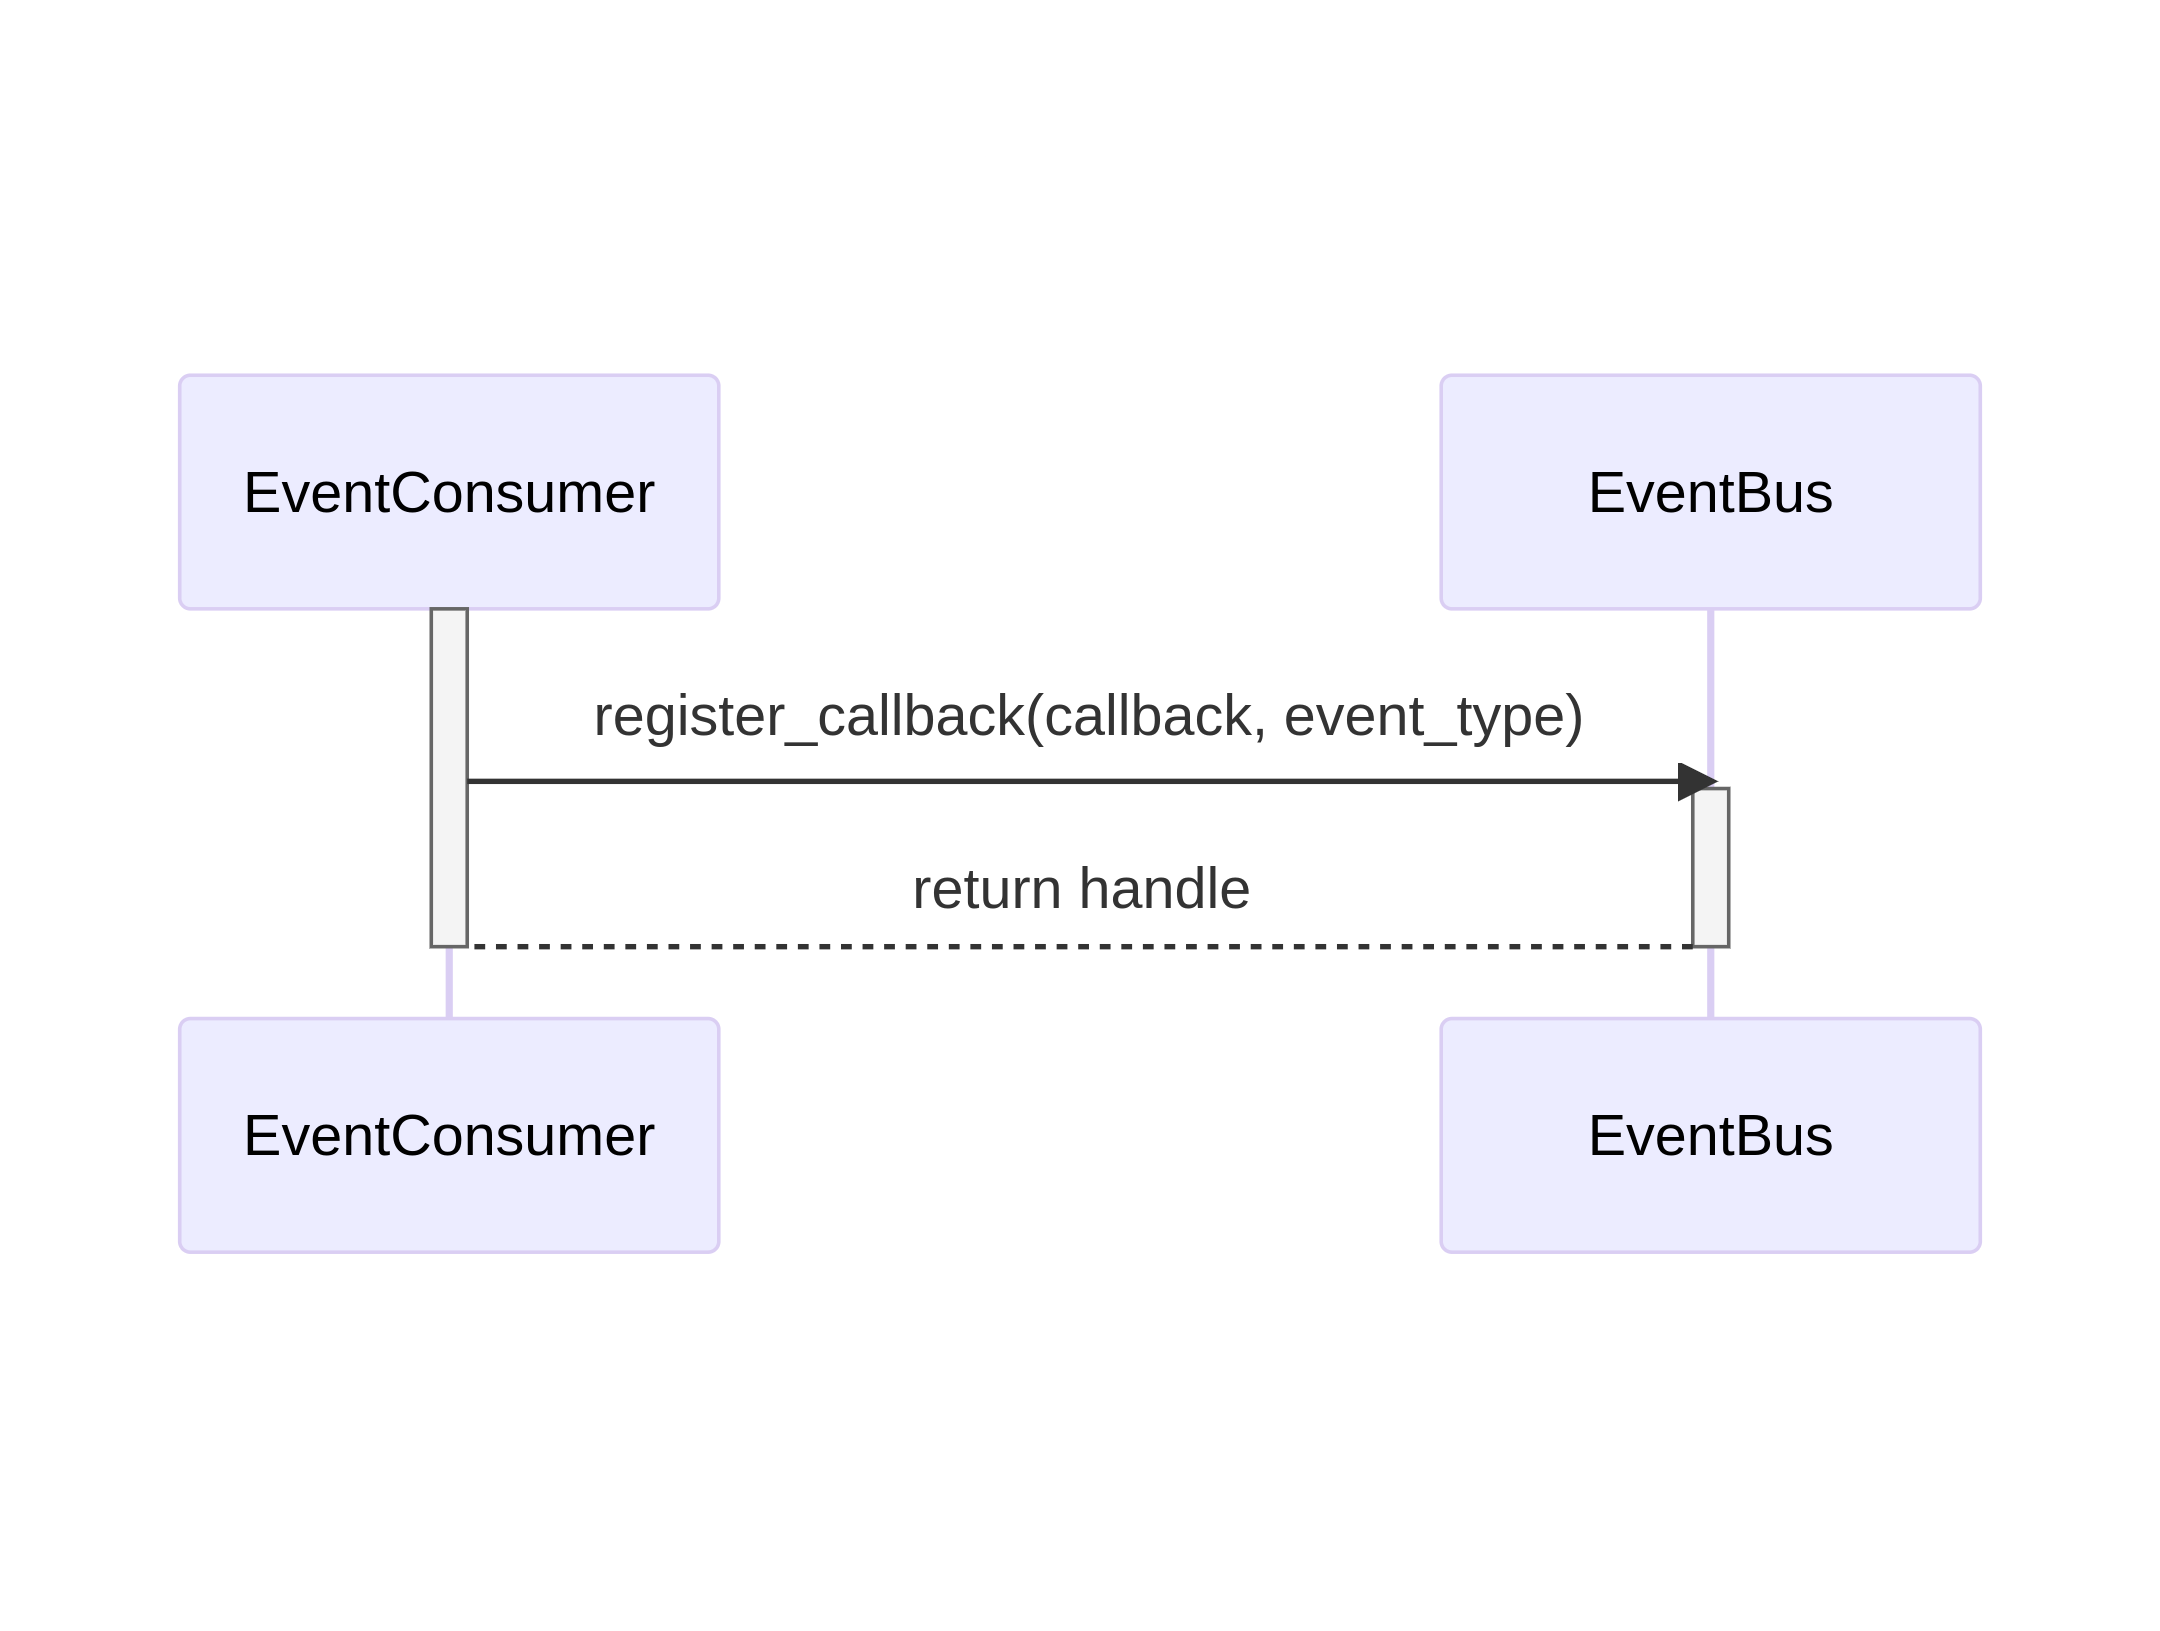
\includegraphics[width=0.75\linewidth]{images/diagrams/eventbus-register-seq.png}
	\caption{Sequenzdiagramm der Registrierung eines Empfängers beim Eventbus.}
	\label{fig:eventbus-register-seq}
\end{figure}

\begin{figure}[!ht]
	\centering
	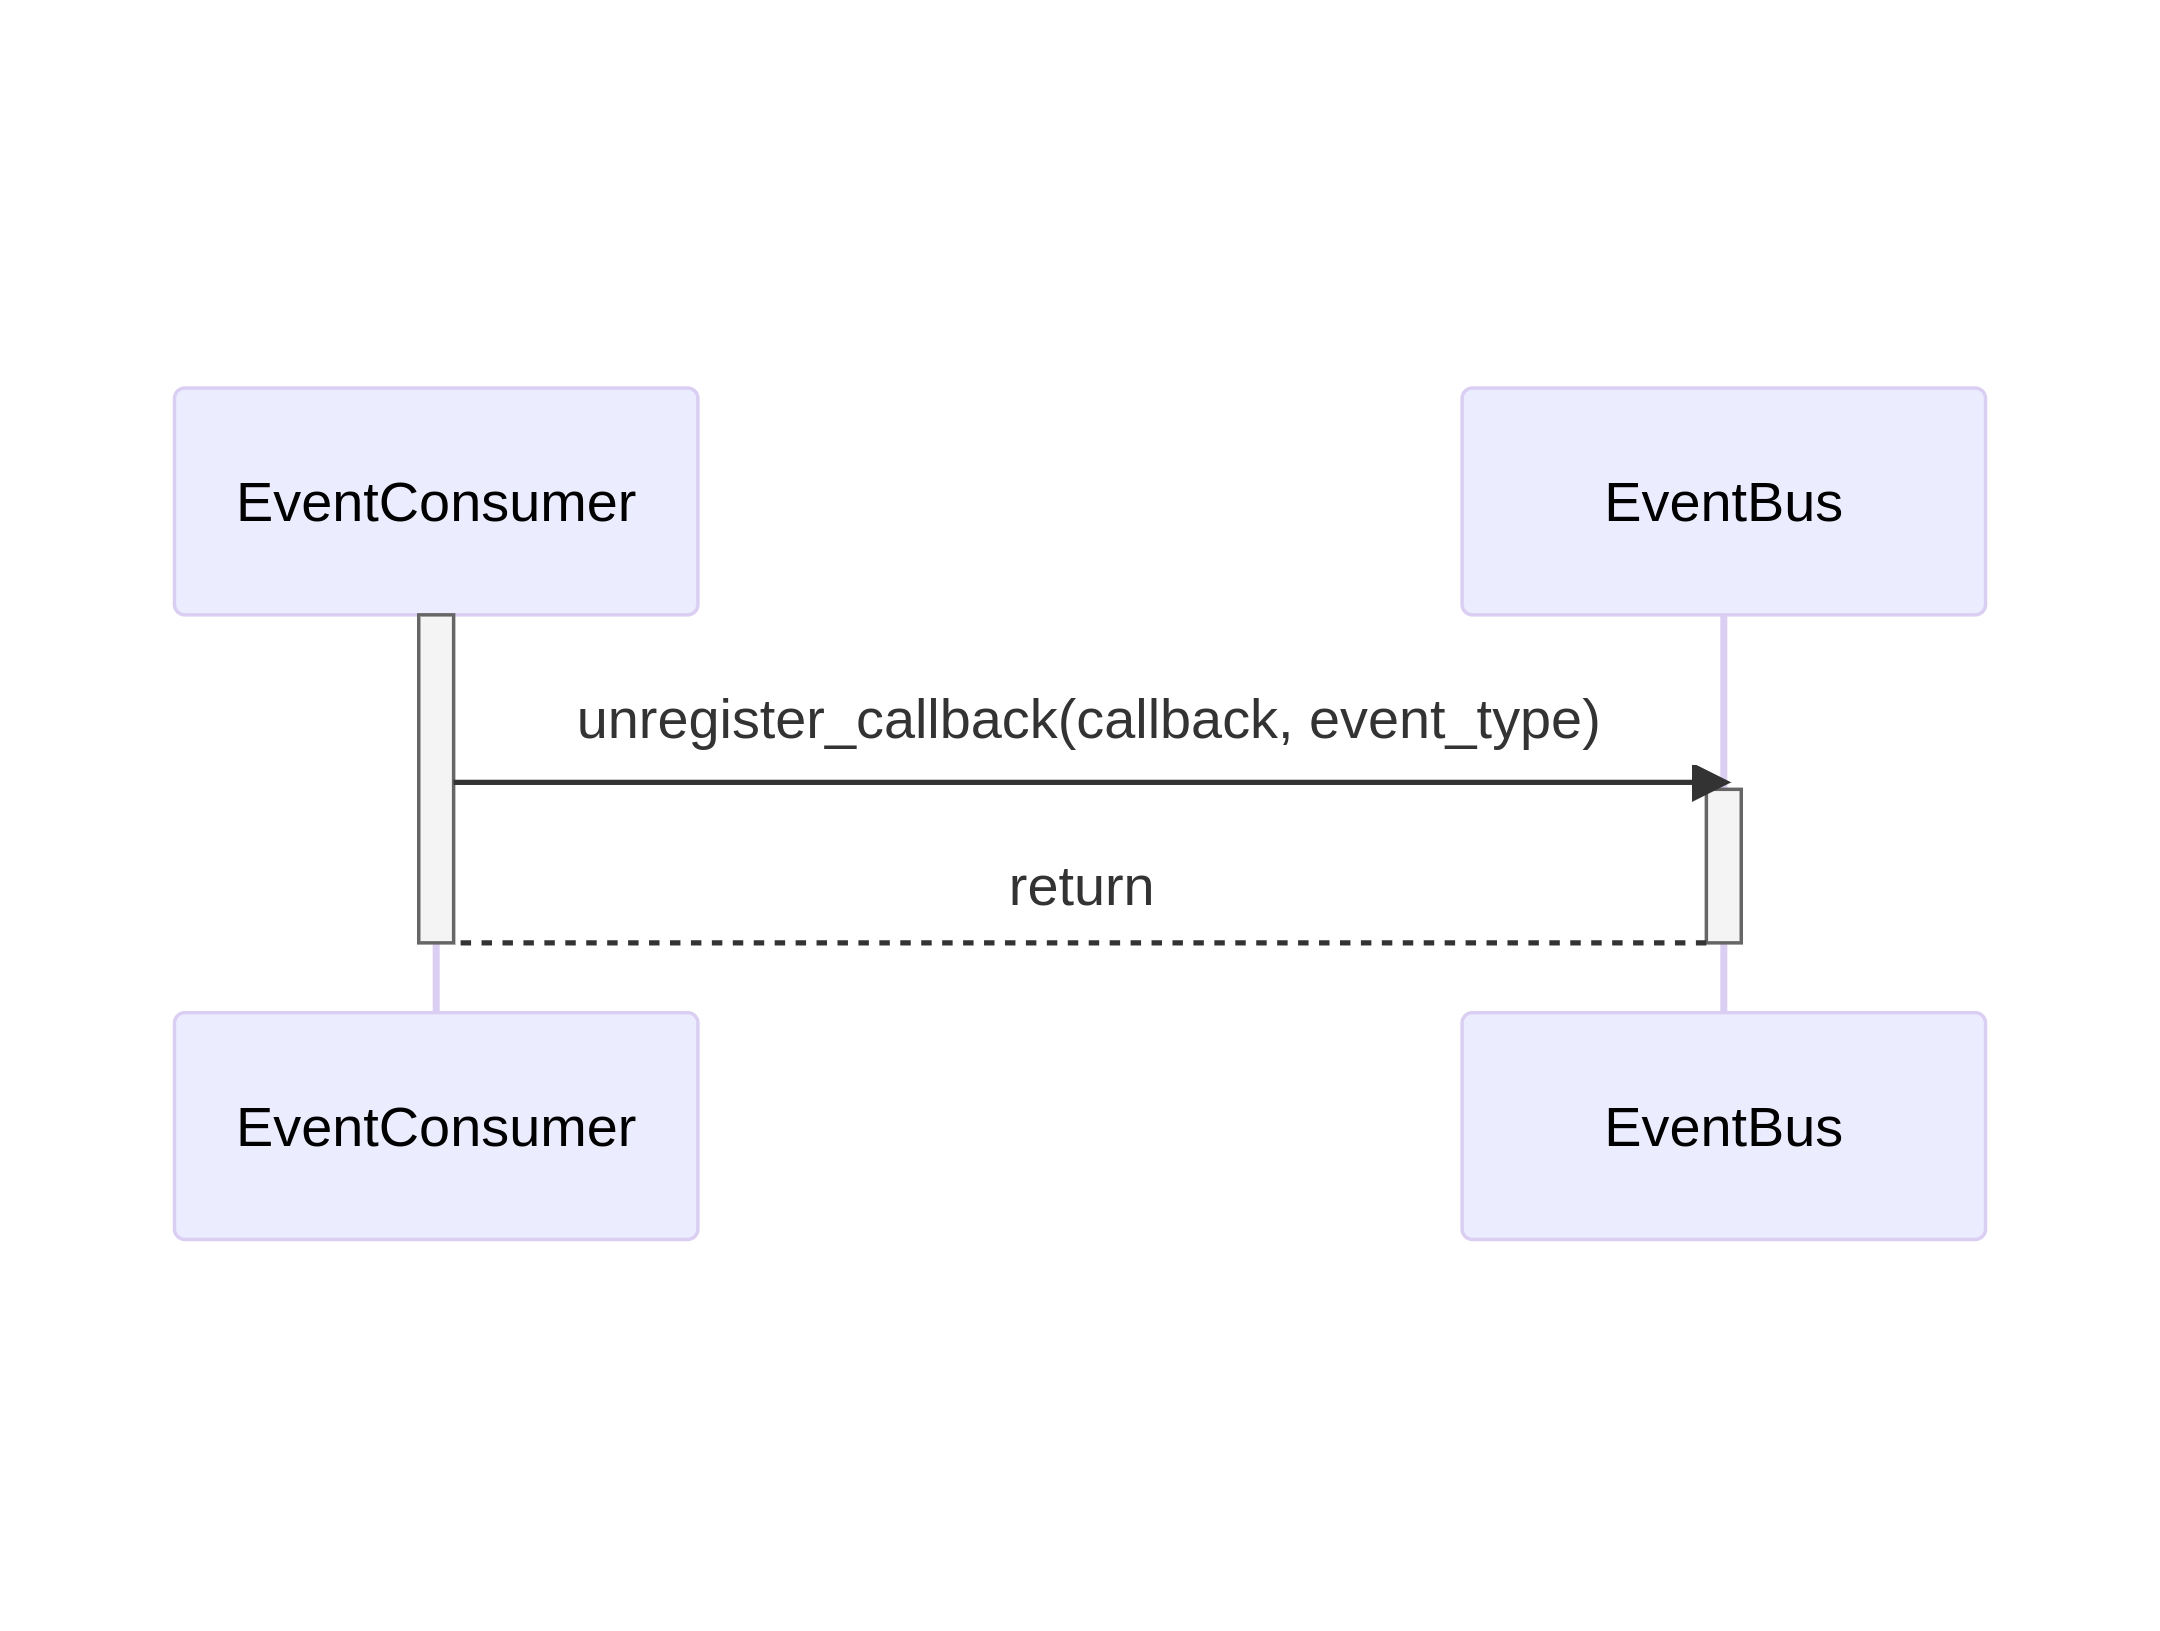
\includegraphics[width=0.75\linewidth]{images/diagrams/eventbus-unregister-seq.png}
	\caption{Sequenzdiagramm der Deregistrierung eines Empfängers beim Eventbus.}
	\label{fig:eventbus-unregister-seq}
\end{figure}

Die Implementierung des Eventbus erfolgte vergleichsweise spät im Projektverlauf. Die Codebasis war bereits entsprechend groß, was uns vor die Herausforderung stellte, wie der Eventbus am besten zu integrieren sei. Auch spielte die Zeitplanung dabei eine Rolle.\\
\\
Da der \emph{Logger} \cite{reisener_entwurf_2023} bereits die Aufgabe übernahm, Ereignisse zu sammeln, lag der Gedanke nahe, ihn entsprechend zu erweitern. Diese Möglichkeit ist im Folgenden unter ''Variante 1 - Erweiterung des \emph{Loggers}'' beschrieben.\\
\\
Da diese Variante gewisse Nachteile mit sich bringt, wird unter ''Variante 2 - Eigenständige Komponente'' eine architektonisch sauberere Lösung vorgestellt. Für diese zweite Lösung haben wir uns aus unten genannten Gründen letztendlich entschieden.

\subsubsection*{Variante 1 - Erweiterung des \emph{Loggers}}

Bei dieser Variante wird das System des \emph{Loggers} erweitert, um die Aufgaben des Eventbus zu übernehmen. Wie \autoref{fig:eventbus-v1-class} zeigt, erstellt der \emph{Logger} für jedes Ereignis ein \code{LogEntry}-Objekt, welches in die Datenbank geschrieben wird. Das \code{LogEntry}-Objekt erbt daher von \code{BaseModel} und besitzt eine \code{save}-Methode, welche bei Erzeugung des Objektes stets ausgeführt wird. Darin wird der Eventbus benachrichtigt, welcher dann die registrierten Empfänger über das neue Ereignis informiert. Die Empfänger realisieren dazu die \code{IEventConsumer}-Schnittstelle, welche eine \code{on\_event}-Methode zur Ereignisbehandlung und ein \code{event\_handle}-Attribut zur Referenzierung der Registrierung beim \code{EventBus} bereitstellt. Die registrierten \emph{Callbacks} werden im Attribut \code{callbacks} gehalten. Es handelt sich dabei um eine Liste von 2-Tupeln, welche das \emph{Callback} und den Ereignistyp enthalten. Ein \emph{Callback} nimmt dabei ein \code{LogEntry}-Objekt entgegen und hat keinen Rückgabewert.

\begin{figure}[!ht]
	\centering
	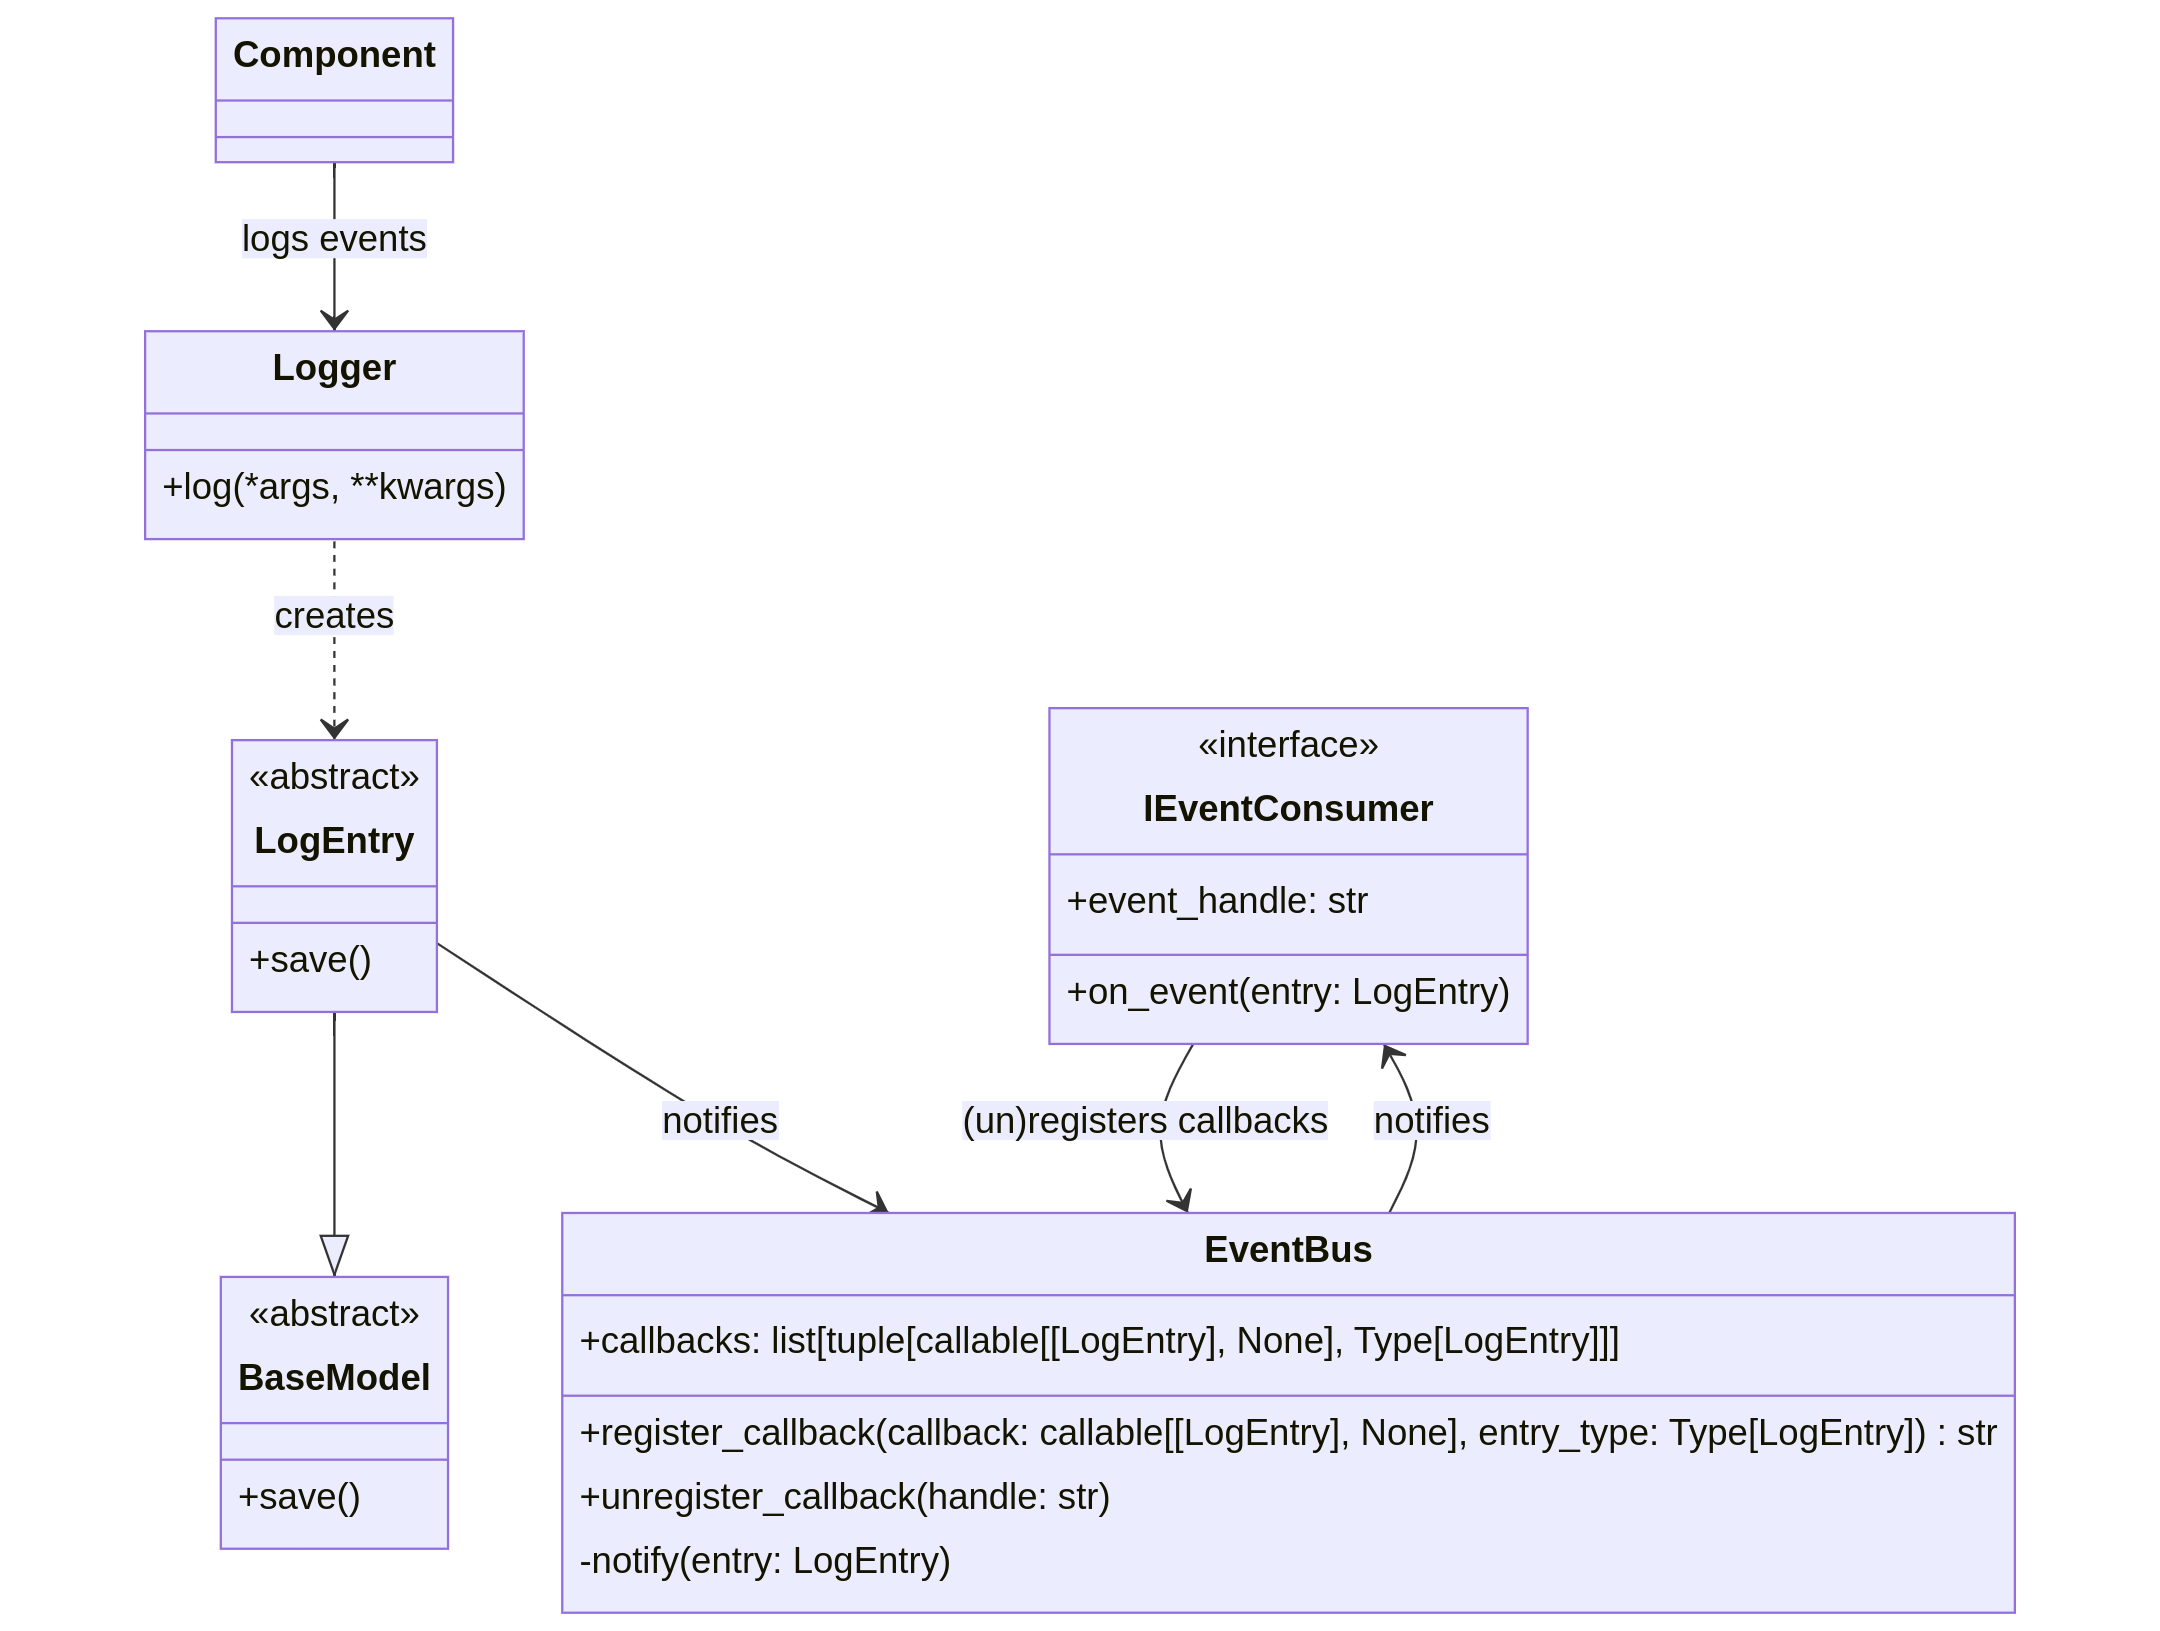
\includegraphics[width=1.0\linewidth]{images/diagrams/eventbus-v1-class.png}
	\caption{Klassendiagramm der ersten Variante des Eventbus.}
	\label{fig:eventbus-v1-class}
\end{figure}

\autoref{fig:eventbus-v1-seq} zeigt den Vorgang der Meldung eines Ereignisses an den \emph{Logger} bis hin zur Benachrichtigung der abhängigen Empfänger. Eine Komponenten (\code{Component}) sendet ein Ereignis durch Aufruf von \code{log} an den \code{Logger} (1). Dieser erzeugt durch \code{create} ein \code{LogEntry}-Objekt (2) und ruft dessen \code{save}-Methode auf (3). Diese benachrichtigt den Eventbus durch Senden von \code{notify} und übergibt dabei das \code{LogEntry}-Objekt selbst (4). Der Eventbus iteriert über die Liste der registrierten \emph{Callbacks} und ruft für jeden Eintrag das \emph{Callback} auf, sofern der Ereignistyp übereinstimmt (5).\\

\begin{figure}[!ht]
	\centering
	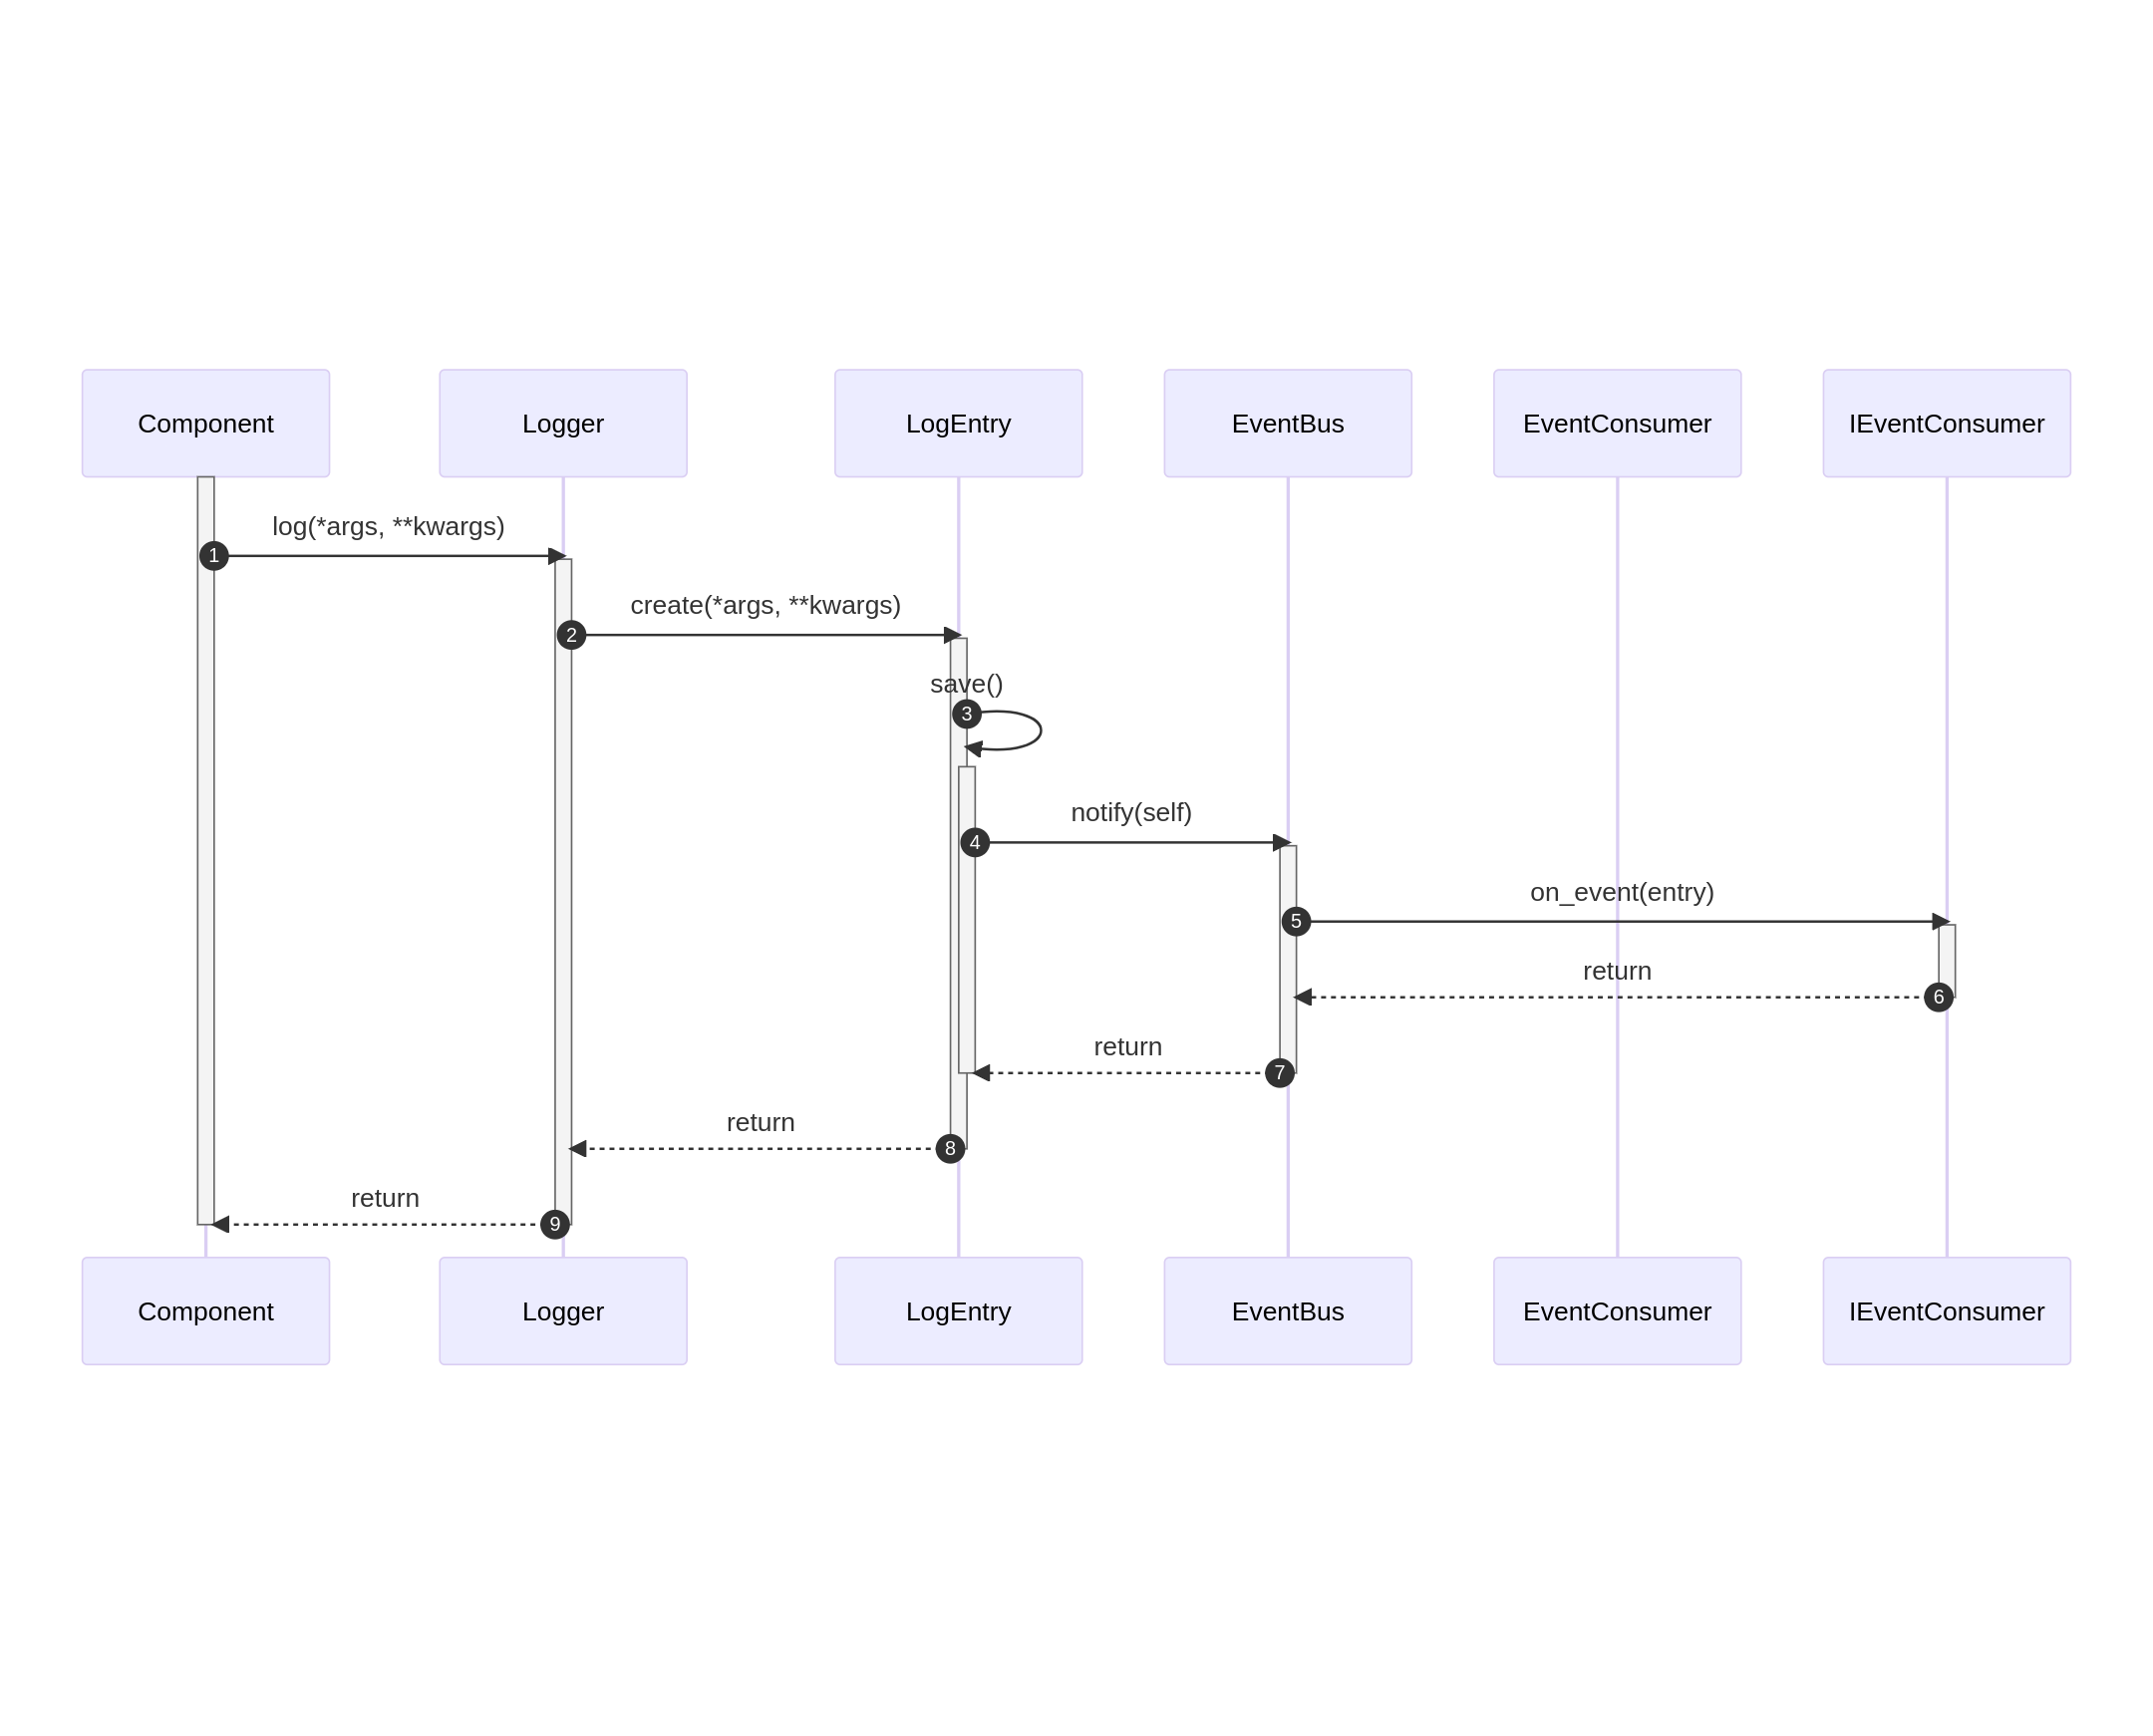
\includegraphics[width=1.0\linewidth]{images/diagrams/eventbus-v1-seq.png}
	\caption{Sequenzdiagramm der ersten Variante des Eventbus.}
	\label{fig:eventbus-v1-seq}
\end{figure}

Der Vorteil dieser Variante ist die einfache Integration in das bestehende System. Die Änderungen am bestehenden Quelltext sind gering. Damit kann die Implementierung des Eventbus schnell erfolgen, was einen positiven Einfluss auf die Zeitplanung hat. Nachteilhaft ist jedoch, dass das \emph{Logging}-System nun auch Teilaufgaben des Eventbus übernimmt. Dies widerspricht dem Prinzip der \emph{Single Responsibility}\footnote{Eine Komponente, Klasse oder Funktion soll nur ein Konzept implementieren oder nur eine Aufgabe erledigen.} und kann zu einer unübersichtlichen Codebasis führen.

\subsubsection*{Variante 2 - Eigenständige Komponente}

Bei dieser Variante wird der Eventbus als eigenständige Komponente implementiert. \autoref{fig:eventbus-v2-class} zeigt das Klassendiagramm. Jede Komponente hält nun eine Referenz auf den Eventbus, um sich als Empfänger registrieren zu können. Die Registrierung und Deregistrierung, sowie die Verwaltung der registrieren \emph{Callbacks} erfolgt wie bei der ''Erweiterung des \emph{Loggers}''. Der Unterschied besteht darin, dass die Ereignisse nun nicht mehr durch \code{LogEntry}-Objekte, sondern durch \code{Event}-Objekte repräsentiert werden. Komponenten benachrichtigen hier selbst den \code{EventBus}. Der \emph{Logger} implementiert die \code{IEventConsumer}-Schnittstelle und registriert sich ebenfalls beim Eventbus, um seine Aufgabe erfüllen zu können.

\begin{figure}[!ht]
	\centering
	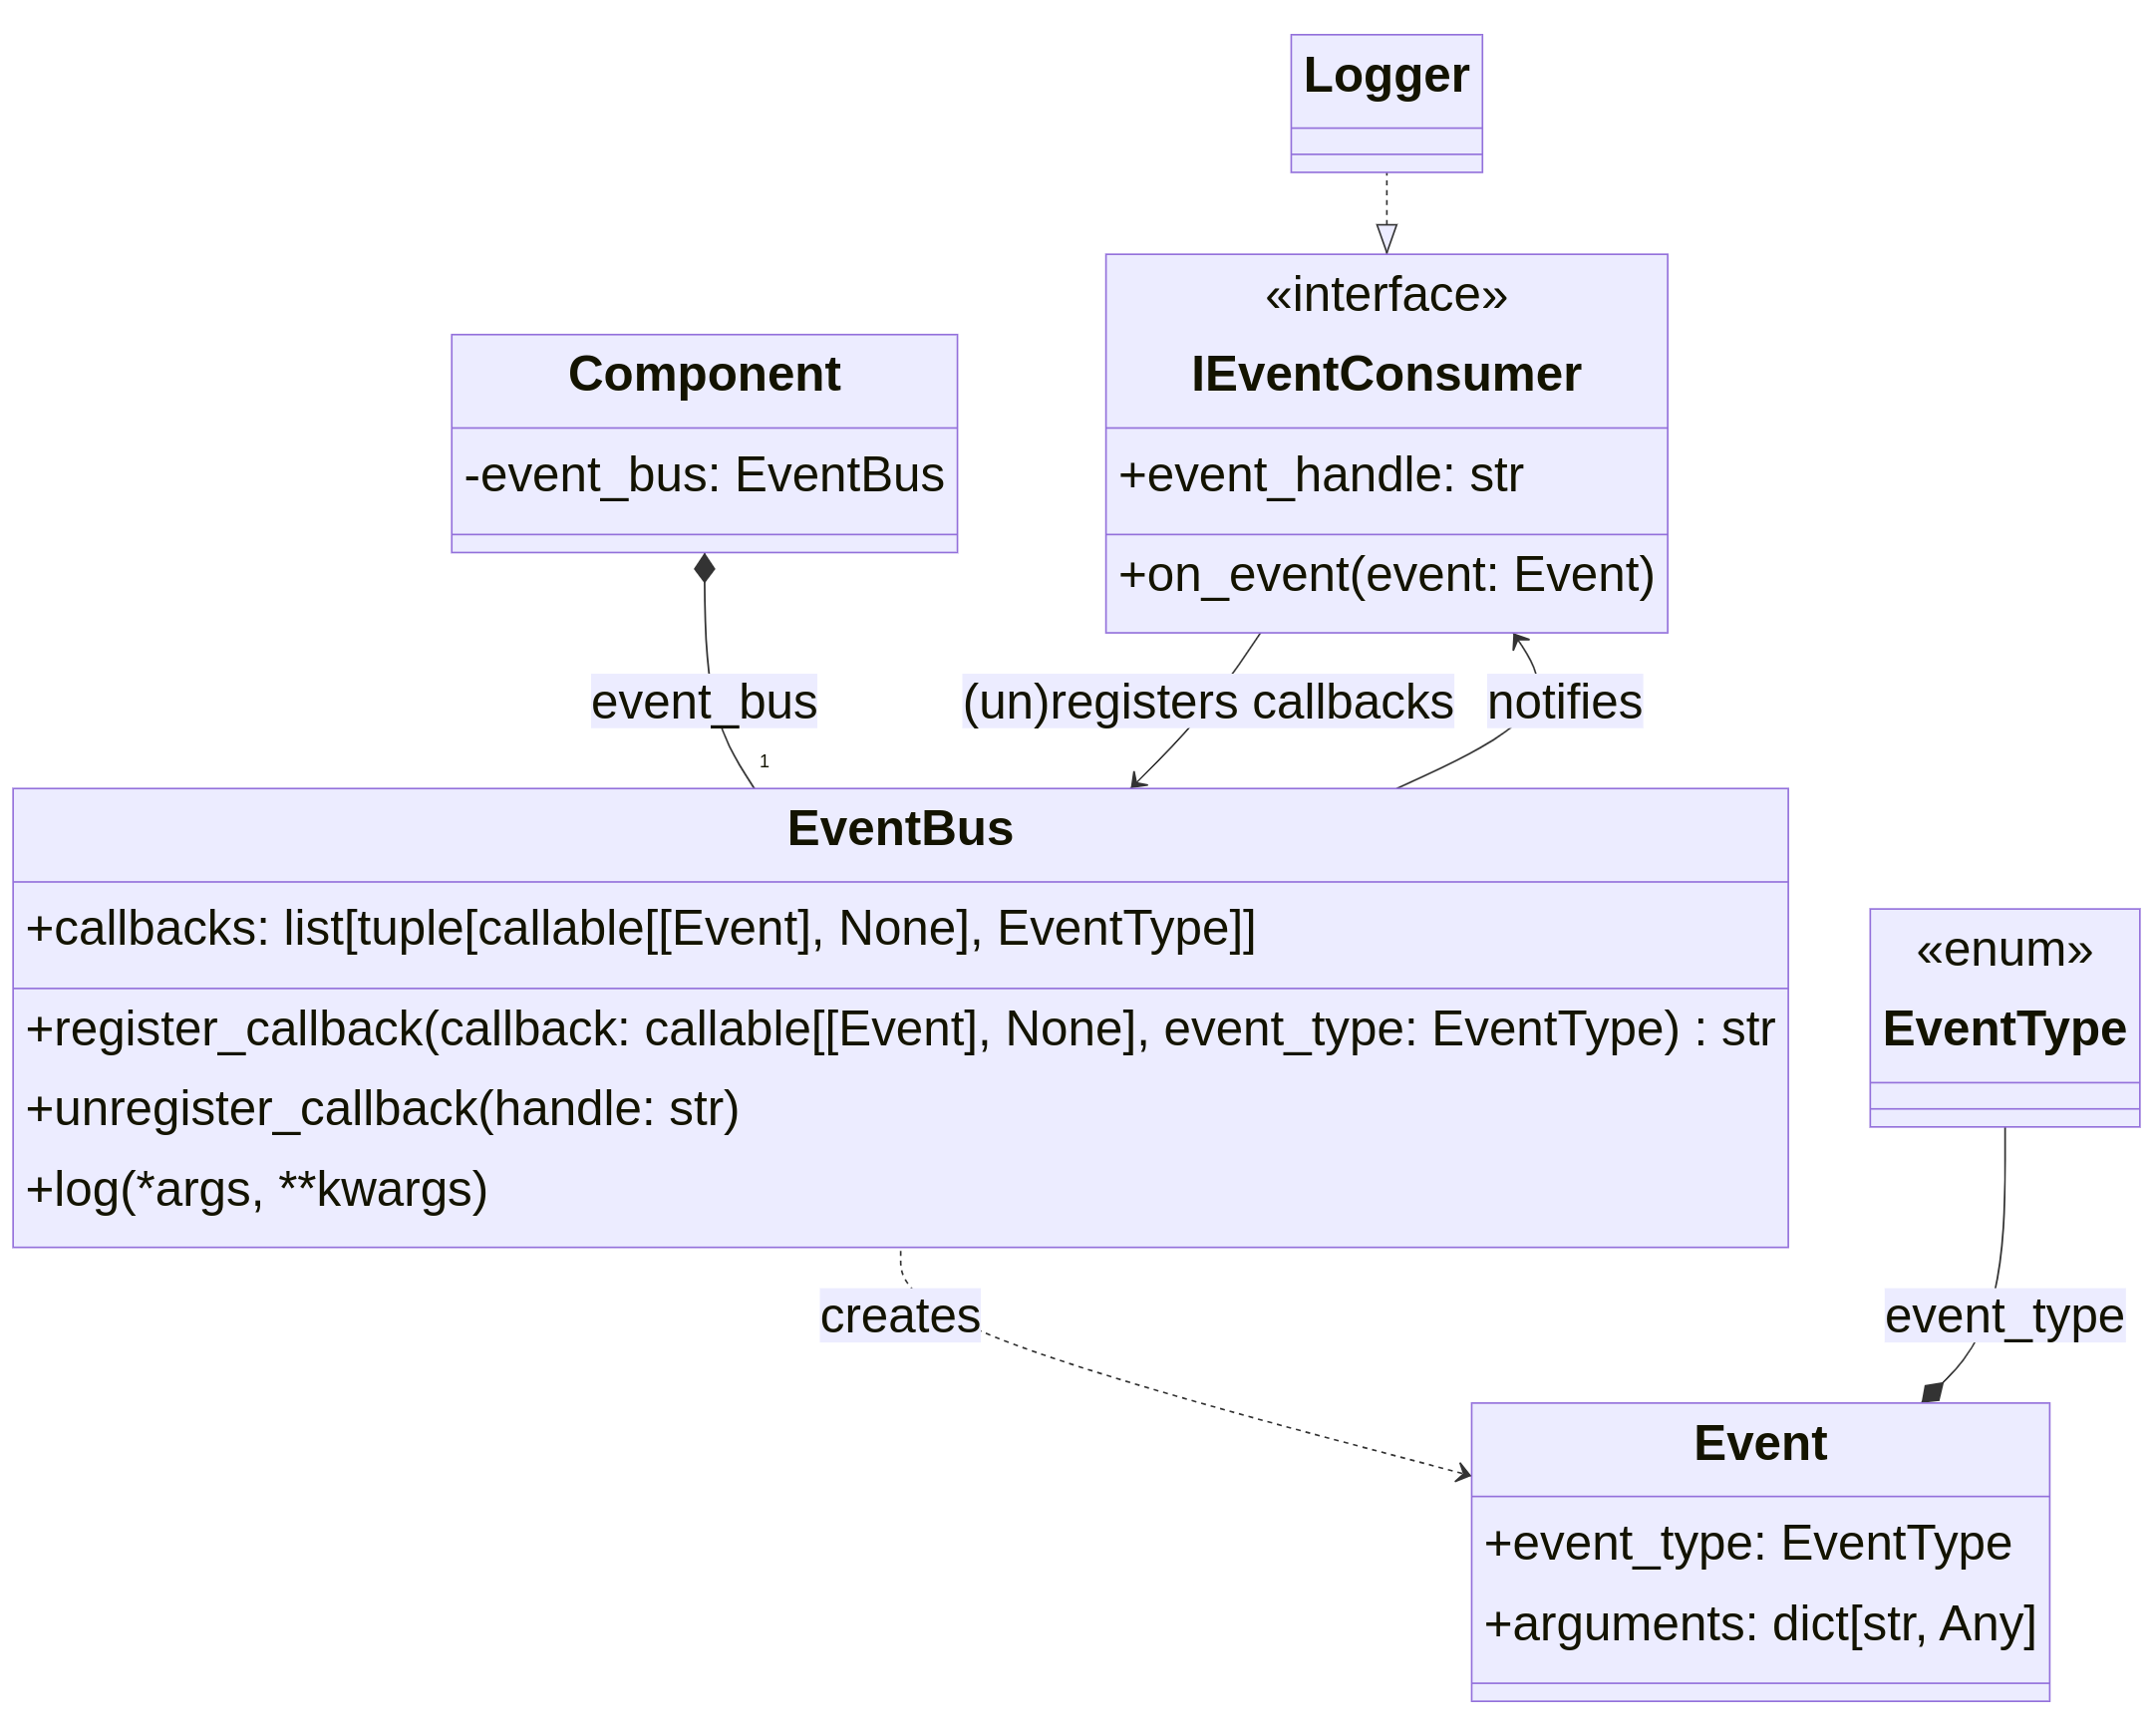
\includegraphics[width=1.0\linewidth]{images/diagrams/eventbus-v2-class.png}
	\caption{Klassendiagramm der zweiten Variante des Eventbus.}
	\label{fig:eventbus-v2-class}
\end{figure}

\autoref{fig:eventbus-v2-seq} zeigt den Ablauf der Meldung eines Ereignisses an den Eventbus. Eine Komponente (\code{Component}) sendet die Parameter eines Ereignisses, durch Aufruf von \code{log}, an den \code{EventBus} (1). Dieser instanziiert ein \code{Event}-Objekt mit den übergebenen Parametern (2). Anschließend iteriert er über die Liste der registrierten \emph{Callbacks} und ruft diese auf, sofern der Ereignistyp übereinstimmt (3).

\begin{figure}[!ht]
	\centering
	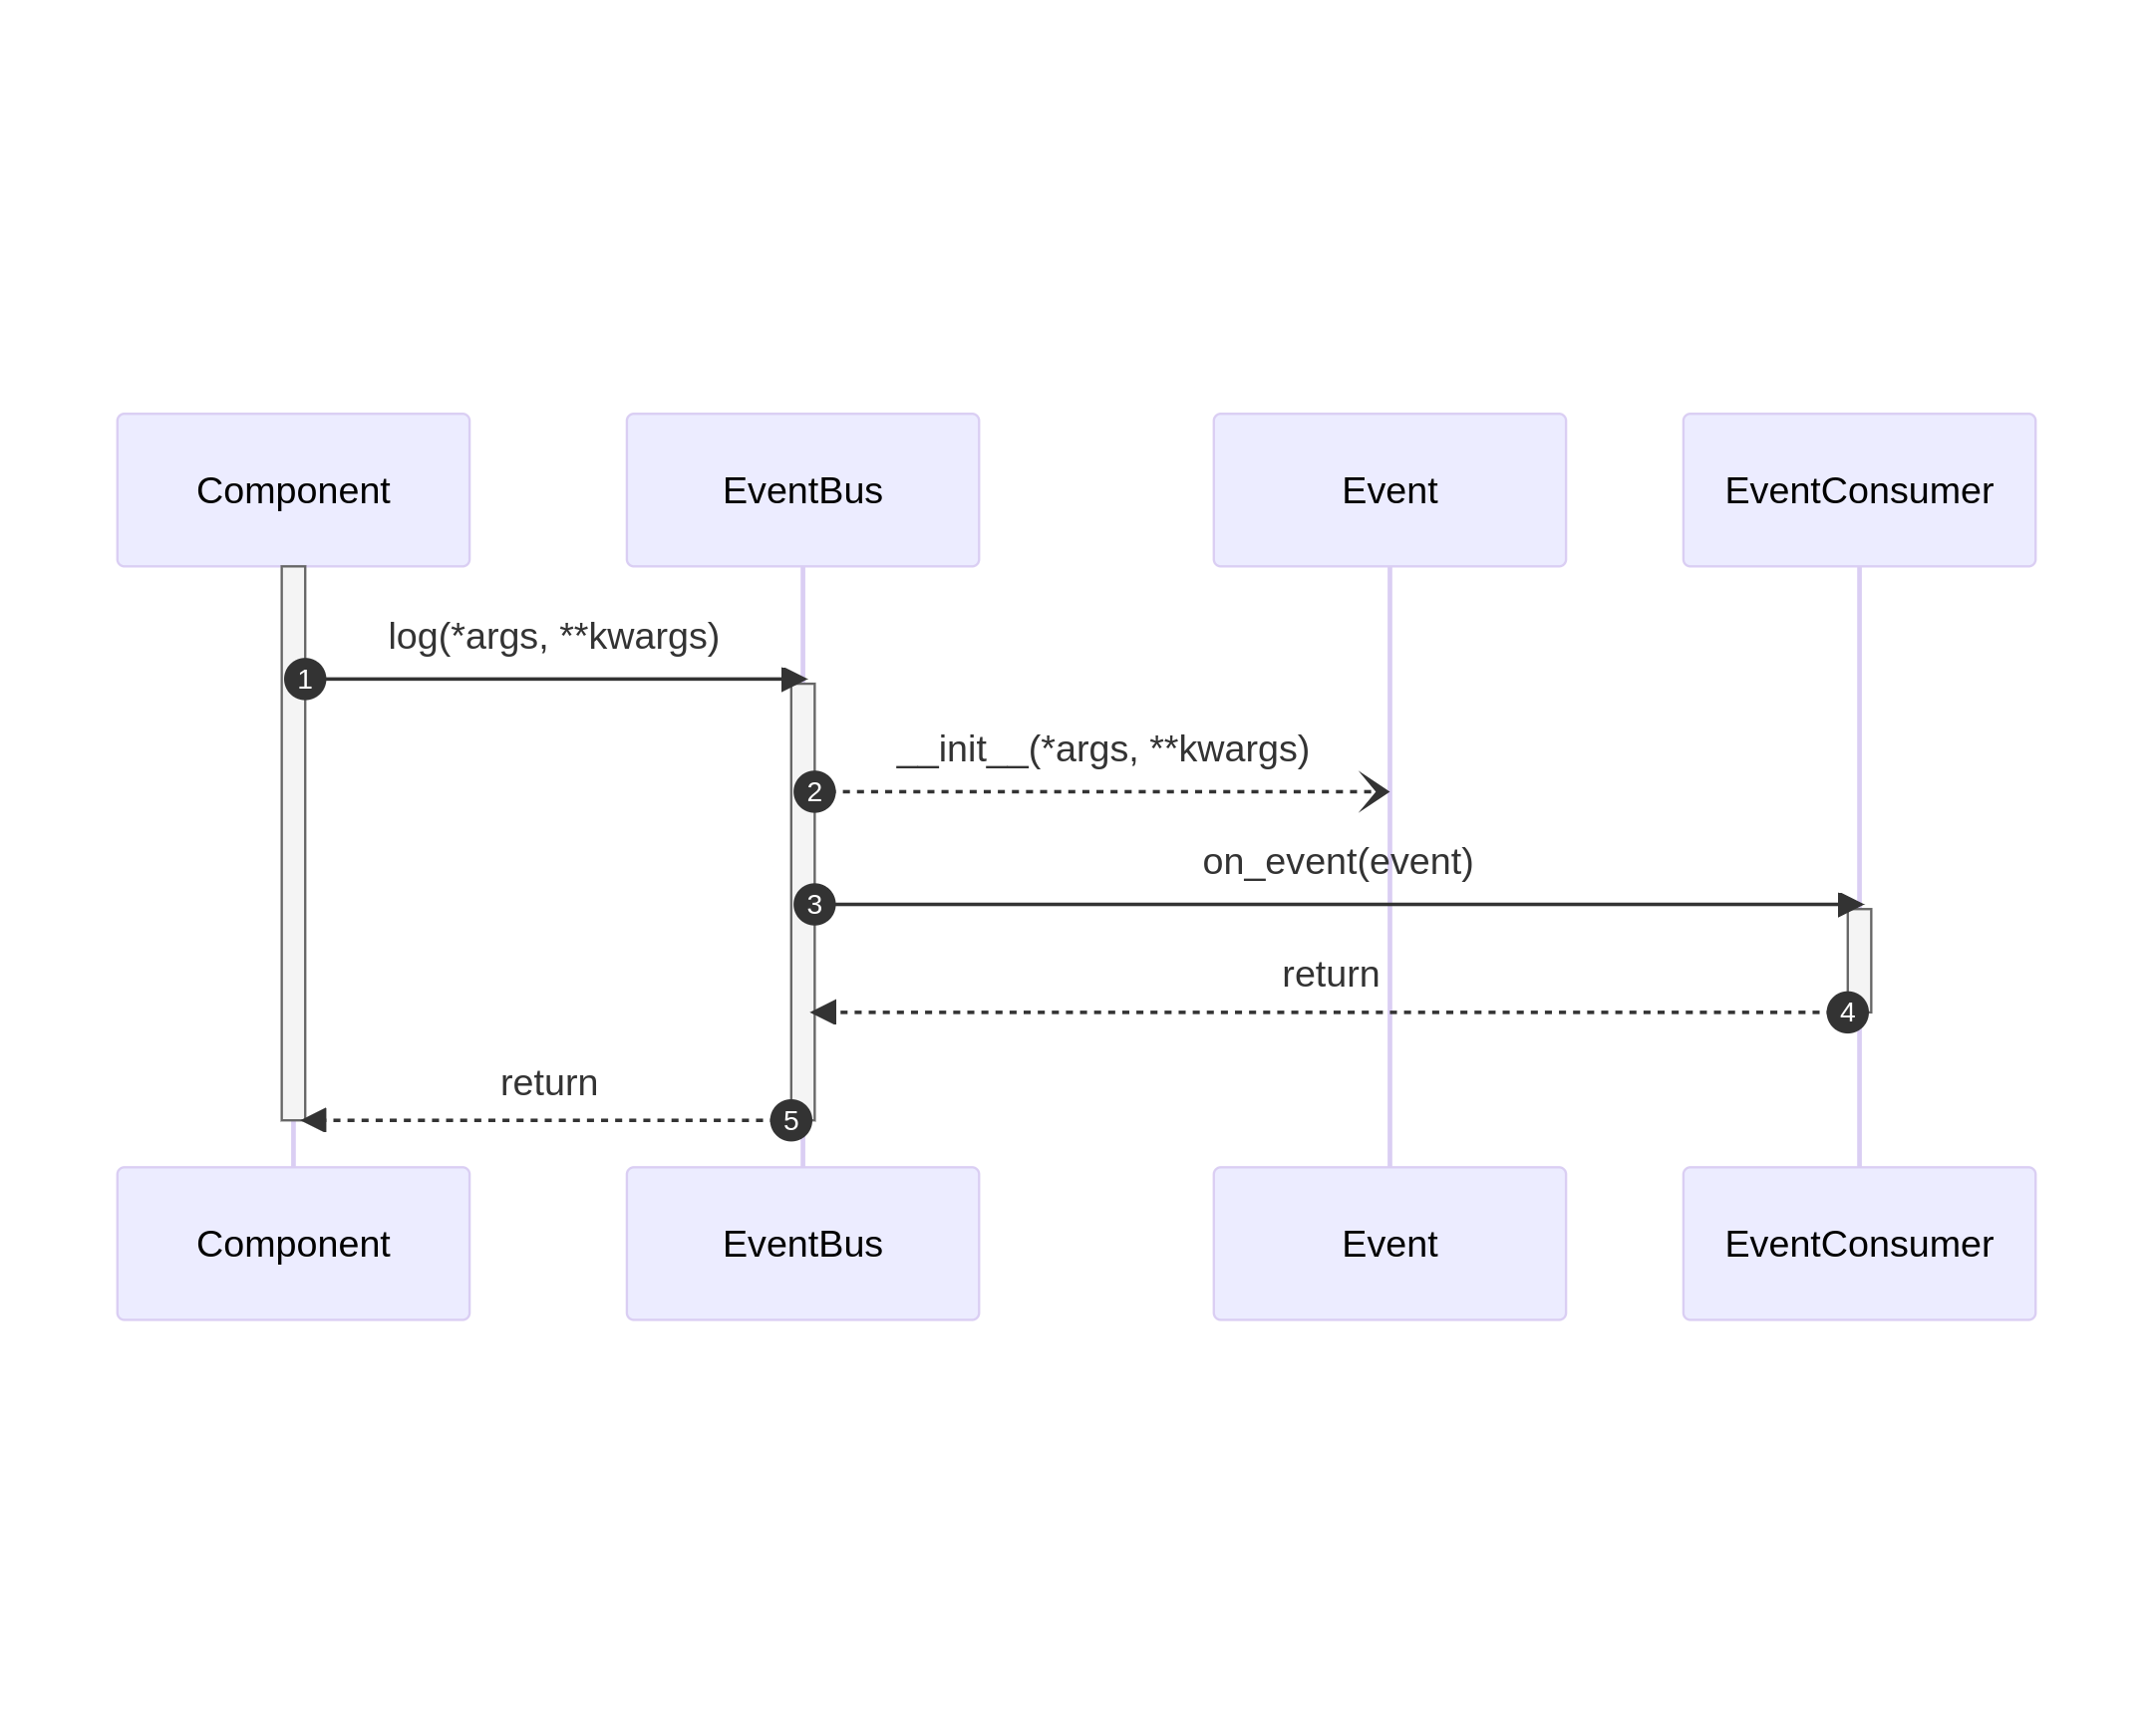
\includegraphics[width=1.0\linewidth]{images/diagrams/eventbus-v2-seq.png}
	\caption{Sequenzdiagramm der zweiten Variante des Eventbus.}
	\label{fig:eventbus-v2-seq}
\end{figure}

Der Vorteil dieser Variante ist die saubere Trennung der Aufgaben des \emph{Loggers} und des Eventbus und die klare Zuordnung der Verantwortlichkeiten. Dafür ist die Implementierung aufwändiger, da mehr Änderungen am bestehenden Quelltext notwendig sind. Das bezieht sich vor allem auf den Umbau des \emph{Loggers}, welcher mit \code{Event}-Objekten statt mit direkt übergebenen Argumenten arbeiten muss. Trotz des Mehraufwandes haben wir uns letztendlich zugunsten der Codequalität für diese Variante entschieden.\\
\\
Eine Verwendung findet der Eventbus im aktuellen System nicht. Aus Zeitgründen wurder der Eventbus zwar implementiert, jedch nicht mehr verwendet. Mögliche Verwendungensind im Ausblick dieser Arbeit beschrieben.

	\section{Implementierungsdetails}
\todo{Deadline: 27.06.}
\todo{Noch in Arbeit}
\todo{Hier zeige ich Code, der interessant sein könnte.}
\todo{FRAGE: Ist es ok, wenn ich nur ''interessanten'' Code zeige? Ansonsten bin ich der Meinung, dass die Sequenzdiagramme und der Text in der Architekturdiskussion das implementierte Verhalten bereits gut beschreibt.}

\subsection{Warteschlange für die Zugerzeugung}
\todo{Noch in Arbeit}

\lstset{language=python}
\begin{lstlisting}[caption={Quelltextunterschrift}, label=code:template-method-code]
class Schedule(ABC):

    _seconds_to_be_spawned: list[int]
    _blocked: bool

    def maybe_spawn(self, seconds: int, spawner: Spawner):
        if not self._blocked and self.strategy.should_spawn(seconds):
            self._seconds_to_be_spawned.append(seconds)

        if len(self._seconds_to_be_spawned) > 0:
            if self._spawn(spawner, self._seconds_to_be_spawned[-1]):
                self._seconds_to_be_spawned.pop()

    @abstractmethod
    def _spawn(self, spawner: Spawner, seconds: int) -> bool:
    	raise NotImplementedError()
\end{lstlisting}

\subsection{Erzeugung bedarfsorientierter Züge}
\todo{Noch in Arbeit}

\lstset{language=python}
\begin{lstlisting}[caption={Quelltextunterschrift}, label=code:template-method-code]
class DemandScheduleStrategy(ScheduleStrategy):
    SECONDS_PER_QUARTER_HOUR: int
    COAL_PER_TRAIN: float

    start_datetime: datetime
    spawn_seconds: list[int]

    def __init__(self, ...):
        ...
        self._calculate_spawn_seconds()
        ...

    def _compute_trains_to_spawn(self, produced_electrical_power: float) -> float:
        coal_consumption = self.compute_coal_consumption(produced_electrical_power)
        return coal_consumption / self.COAL_PER_TRAIN

    def _calculate_spawn_seconds(self):
        end_datetime = self.start_datetime + timedelta(
            seconds=self.end_time - self.start_time
        )
        data = self._api.get_data(self.start_datetime, end_datetime)
        train_accumulator = 0.0
        for quarter_hour, entry in enumerate(data):
            train_accumulator += self._compute_trains_to_spawn(entry.value)
            seconds = int(quarter_hour * self.SECONDS_PER_QUARTER_HOUR + self.start_time)
            while train_accumulator >= 1.0:
                self.spawn_ticks.append(seconds)
                train_accumulator -= 1.0
                tick += 1

	def should_spawn(self, seconds: int) -> bool:
    	return super().should_spawn(seconds) and seconds in self.spawn_seconds
\end{lstlisting}
	\section{Simulationsergebnisse}
\todo{Deadline: 01.07.}
\todo{Sobald wir zuverlässige Ergebnisse produzieren können, mache ich mir hier weiter Gedanken. Es wird aber darauf hinauslaufen, dass ich produzierte Ergebnisse beschreibe und ein paar Diagramme zeige.}

	\chapter{Schlussbetrachtung}
	\section{Architekturübersicht}
\todo{Deadline: 28.06.}
\todo{Noch in Arbeit}
\todo{Hier gebe ich nochmal einen kurzen abschliependen Überblick über die Architektur.}
	\section{Ergebnisdiskussion}
\todo{Deadline: 01.07.}
\todo{Die beschriebenen Ergebnisse werden hier diskutiert und Erkenntnisse werden daraus abgeleitet.}
	\section{Ausblick}
\todo{Deadline: 25.06.}
\todo{Ich zeige, was man in Zukunft noch machen kann / noch hätte machen können. Vor allem ist das im Kontext meiner Arbeit die Nutzung des EventBus für Abfarhtspläne, die auf Ereignisse in der Simulation reagieren.}

	% Bibliographie
	\ifisbook\cleardoubleemptypage\fi
	\phantomsection\addcontentsline{toc}{chapter}{\refname}
	\printbibliography %[category=cited]
	
	% ggf. Anhang
	\appendix\chapter{\appendixname}

\section*{Interview mit Sascha Lesche von der LEAG}

\begin{description}

    \item[Christian Raue:] Lassen Sie uns zunächst zum Thema des Kohletransportes kommen. Wie viele Tonnen Kohle passen in einen Zug?

    \item[Sascha Lesche:] Ein Zug besteht immer aus einer Lok und 16 Wagen. Jeder Wagen hat eine Aufnahmekapazität von 84 Kubikmeter, was 60 Tonnen Kohle entspricht. Damit kommen Sie auf eine Gesamtmenge von 960 Tonnen.

    \item[Christian Raue:] Welchen Energiegehalt hat die transportierte Kohle im Schnitt?

    \item[Sascha Lesche:] Der Energiegehalt der Kohle schwankt. Da sie nicht gleichmäßig gewachsen ist, weist sie teilweise sehr unterschiedliche chemische Zusammensetzungen auf, welche den Energiegehalt beeinflusst. Für eine Faustformel empfehle ich, sich auf allgemeine Quellen zu berufen.

    \item[Max Lietze:] Als Nächstes möchten wir gern mit Ihnen darüber reden, wie wir die Züge in unserer Simulation möglichst realistisch repräsentieren können. Eine Frage ist dabei, wie lang so ein Zug ist.

    \item[Sascha Lesche:] Die Länge eines Wagens beträgt 12,5 Meter. Zusammen mit der Lok kommen Sie dann auf eine Länge von ca. 220 Metern.

    \item[Max Lietze:] Wie schnell kann ein Kohlezug fahren?

    \item[Sascha Lesche:] Die Loks schaffen eine Geschwindigkeit von 60 km/h, dürfen aber gemäß Bau- und Betriebsanweisung maximal 50 km/h fahren.

    \item[Max Lietze:] Wie schnell könne die Züge beschleunigen und abbremsen?

    \item[Sascha Lesche:] Es gibt zunächst sogenannte Zuglastdiagramme, bei welchen die Zugkraft in Zusammenhang mit der Masse gebracht wird. Wahrscheinlich wird es aber schwierig sein, die Werte daraus abzuleiten. Ich kann Ihnen jedoch theoretische Annahmen geben. Für die Beschleunigung wären das 0,15 Meter pro Quadratsekunde und für das Abbremsen 0,4 Meter pro Quadratsekunde.

    \item[Max Lietze:] Wie lange dauert das Be- und Entladen?

    \item[Sascha Lesche:] Das Be- und Entladen dauert zwischen 20 und 30 Minuten. Wenn Sie ihr System stabil laufen lassen wollen, sollten Sie vielleicht besser von 30 Minuten ausgehen.

    \item[Christian Raue:] Wir möchten unsere Simulationsergebnisse gern mithilfe von Echtweltdaten verifizieren. Können Sie uns sagen, in welchem Takt die Züge im Mittel in den Kraftwerken ankommen?

    \item[Sascha Lesche:] Vor vielen Jahren, fuhren die Kraftwerke noch eine reine Grundlast. Da hätte man ein Tagesmittel angeben können. Im Moment ist das nicht möglich. Es gibt je nach Bedarf große Schwankungen. Am Tag können 80 Züge in ein großes Kraftwerk einfahren. Manchmal sind es mehr, bei entsprechend geringeren Leistungen auch weniger.

    \item[Christian Raue:] Wie viele Züge befinden sich im Schnitt gleichzeitig auf dem Schienennetz?

    \item[Sascha Lesche:] Das ist leider genauso schwer zu beantworten. Es können zehn bis zwanzig Züge sein. Bei 25 Zügen ist dann aber langsam ein Limit erreicht, von Reststoff- und Transportfahrten abgesehen.

\end{description} % example
	
	% ggf. bei englischen Arbeiten den deutschen Abstract nach hinten verschieben
	% \ifisbook\pagestyle{plain}\cleardoubleemptypage\include{content/abstract_deu}\fi

	% Eigenständigkeitserklärung
	\ifisbook\pagestyle{plain}\cleardoubleemptypage% => Laut Aussage des Studienreferats braucht es - auch wenn die Arbeit in englischer Sprache verfasst ist - KEINE separate Version der Eigenständigkeitserklärung auf Englisch. Sowohl für Arbeiten in deutscher Sprache als auch für Arbeiten in englischer Sprache genügt EINE EINZIGE Eigenständigkeitserklärung auf DEUTSCH.
\begin{otherlanguage}{ngerman}

\begin{center}\textsf{\textbf{Eidesstattliche Erklärung}}\end{center}
Hiermit versichere ich, dass meine {\hpitype} \enquote{\hpititle} (\enquote{\hpititleother}) selbständig verfasst wurde und dass keine anderen Quellen und Hilfsmittel, als die angegebenen benutzt wurden. Diese Aussage trifft auch für alle Implementierungen und Dokumentationen im Rahmen dieses Projektes zu.\\

\noindent
Potsdam, den \hpidate,
\vspace{2cm}

\begin{center}
\begin{tabular}{C{6cm}}
\hline
{\small({\hpiauthor})}
\end{tabular}
\end{center}

\end{otherlanguage}


\fi

\end{document}